%%%%%%%%%%%%%%%%%%%%%%%%%%%%%%%%%%%%%%%%%%%%%%%%%%%%%%%%%%%%%%%%%%%%%
% NUEN 410 Nuclear Engineering Systems and Design
% Design Project Review Template
% Texas A&M University - Department of Nuclear Engineering
%%%%%%%%%%%%%%%%%%%%%%%%%%%%%%%%%%%%%%%%%%%%%%%%%%%%%%%%%%%%%%%%%%%%%

\documentclass[12pt]{article}
\setlength{\parindent}{0pt}
\setlength{\parskip}{12pt}
% Packages
\usepackage[margin=1in]{geometry}
\usepackage{setspace}
\usepackage{tabularx}

% --- column types --------------------------------------------
\newcolumntype{L}[1]{>{\raggedright\arraybackslash}p{#1}}
\newcolumntype{R}[1]{>{\raggedleft\arraybackslash}p{#1}}
\newcolumntype{C}[1]{>{\centering\arraybackslash}p{#1}}

% --- markers -------------------------------------------------
\newcommand{\Src}{\,\textcolor{NavyBlue}{\textsuperscript{\textbf{[S]}}}}
\newcommand{\Est}{\,\textcolor{Amber}{\textsuperscript{\textbf{[E]}}}}
\newcommand{\Elim}{\textbf{---}}

\usepackage{graphicx}
\usepackage{subcaption}
\usepackage{makecell}
\usepackage{array}
\usepackage{amsmath}
\usepackage{amssymb}
% \usepackage{cite}
\usepackage{hyperref}
\usepackage{fancyhdr}
\usepackage{fancybox}
\usepackage{wasysym}
\usepackage{lastpage}
\usepackage{array}
\usepackage{booktabs}
\usepackage{xcolor}
\usepackage{listings}
\numberwithin{equation}{section}
\usepackage{caption}
\usepackage{float}
\usepackage{svg}
\usepackage{csquotes}
\usepackage{longtable}
\usepackage[backend=biber,style=ieee]{biblatex}
\addbibresource{references.bib}
\addbibresource{references-2.bib}
\usepackage{pdfpages}


% Formatting
\singlespacing  % Single spacing as per requirements (adjust to \singlespacing if needed)
\let\originaleqref\eqref
\renewcommand{\eqref}[1]{Eq.\originaleqref{#1}}
\usepackage[justification=centering]{caption}

% Header and Footer
\newcommand\blfootnote[1]{%
  \begingroup
  \renewcommand\thefootnote{}\footnote{#1}%
  \addtocounter{footnote}{-1}%
  \endgroup
}

\fancyhf{}
\rhead{NUEN 410 Project Review}
\lhead{Team 3}
\cfoot{\thepage\ of \pageref{LastPage}}
\renewcommand{\headrulewidth}{0.4pt}

% Title formatting
\newcommand{\projecttitle}[1]{{\Large\bfseries\centering #1\par}}
\newcommand{\sectionheading}[1]{{\large\bfseries #1}\par\medskip}

% --- colours -------------------------------------------------
\definecolor{NavyBlue}{RGB}{24,95,165}
\definecolor{ForestGreen}{RGB}{15,110,86}
\definecolor{Amber}{RGB}{155,65,10}
\definecolor{RowGray}{RGB}{246,246,246}
\definecolor{RowMid}{RGB}{218,218,218}
\definecolor{HeaderBar}{RGB}{24,95,165}
%%%%%%%%%%%%%%%%%%%%%%%%%%%%%%%%%%%%%%%%%%%%%%%%%%%%%%%%%%%%%%%%%%%%%
% DOCUMENT BEGINS HERE
%%%%%%%%%%%%%%%%%%%%%%%%%%%%%%%%%%%%%%%%%%%%%%%%%%%%%%%%%%%%%%%%%%%%%

\begin{document}

% ===================================================================
% TITLE PAGE
% ===================================================================
\pagestyle{empty}

% TITLE PAGE
\begin{titlepage}
\centering

\vspace*{1in}

% Course Information
{\Large\bfseries NUEN 410}\\[0.4em]
{\large Design of Nuclear Reactors}\\[0.2em]
{\normalsize Spring 2026}

\vspace{1.5in}

% Main Title
{\fontsize{42}{50}\selectfont\bfseries 
LAST BREATH\\[0.2em]
REACTOR DESIGN\par}

\vspace{0.5in}

% Subtitle
{\LARGE\itshape Senior Design Project Review\par}

\vfill

% Institution
{\large 
Submitted to the\\[0.3em]
\textbf{Department of Nuclear Engineering}\\[0.2em]
Texas A\&M University}

\newpage
% Team Members
{\large\bfseries Team Members}\\[0.8em]
{\large
Dylan J. Frank\\[0.5em]
Ridwan T. Imam\\[0.5em]
Sean A. Yeatts
}

\vspace{1in}


% Team Captain and Date
{\normalsize
\textbf{Team Captain:} Dylan J. Frank\\[0.5em]
\textbf{Date:} \today
}

\vspace{0.5in}

\end{titlepage}

\clearpage
% ===================================================================
% Approval
% ===================================================================

\thispagestyle{empty}

\begin{center}
    {\large Approval Page}
\end{center}

\vspace{1.5cm}

\noindent This Design Project Report has been approved by:

\vspace{2cm}

% --- Technical Advisor ---
\noindent\begin{minipage}[t]{0.35\textwidth}
    \vspace{0pt}
    Technical Advisor:\par
    \vspace{1.8cm}
    \hrule
    \vspace{4pt}
    \small Signature
\end{minipage}%
\hfill
\begin{minipage}[t]{0.55\textwidth}
    \vspace{3.5cm}
    \noindent Name (Print)\enspace\underline{\hspace{6cm}}\par
    \vspace{0.5cm}
    \noindent Date\enspace\underline{\hspace{6.5cm}}
\end{minipage}

\vspace{3cm}

% --- Faculty Advisor ---
\noindent\begin{minipage}[t]{0.35\textwidth}
    \vspace{0pt}
    Faculty Advisor:\par
    \vspace{1.8cm}
    \hrule
    \vspace{4pt}
    \small Signature
\end{minipage}%
\hfill
\begin{minipage}[t]{0.55\textwidth}
    \vspace{3.5cm}
    \noindent Name (Print)\enspace\underline{\hspace{6cm}}\par
    \vspace{0.5cm}
    \noindent Date\enspace\underline{\hspace{6.5cm}}
\end{minipage}

\clearpage
% ===================================================================
% EXECUTIVE SUMMARY
% ===================================================================
\section*{Executive Summary (All)}

The U.S. commercial nuclear fleet has discharged over 90,000 metric tons of spent PWR fuel, most of which sits in interim storage with no clear disposal pathway. The \textit{Last Breath Reactor} (LBR) is a heavy-water-moderated reactor concept designed to take that spent fuel --- as-is, without decladding or chemical reprocessing --- and extract an additional 15\,MWd/kgHM of energy from it while reducing its $^{239}$Pu inventory. The core idea is simple: heavy water's near-zero thermal absorption cross section ($\sigma_a \approx 0.001$\,b) is what makes criticality on deeply depleted fuel possible at all. Light water cannot do this at any lattice geometry; D$_2$O can.

The design was driven by three requirements: a $\geq$20\% reduction in per-assembly $^{239}$Pu, sustained criticality through 60\,GWd/tHM of accumulated burnup, and a 2\,GW$_\text{th}$ thermal output within regulatory safety margins. All three have been met.

The 6\,cm square lattice pitch emerged from an OpenMC parametric sweep as the design point that best balances spectrum thermalization, initial excess reactivity, and thermal-hydraulic feasibility. It is a large pitch by any reactor standard, and that has consequences --- the coolant mass flux drops to about 102.6\,kg/m$^2$s, roughly an order of magnitude below a conventional PWR, which cuts the convective heat transfer coefficient to $\sim$757\,W/m$^2$K. Managing heat removal at this pitch is the central engineering challenge of the concept.

The bigger neutronics problem turned out to be the axial burnup profile of spent PWR rods. The midplane is deeply depleted; the rod ends are not. A uniform lattice depletes unevenly as a result, and criticality is lost well before 60\,GWd/t. The solution developed here is the \textit{Fueled Power Inverter} (PI-F): a fresh UO$_2$ rod with a graded enrichment profile (3.5\,wt.\% center / 4.5\,wt.\% edge) placed at 25 of 225 positions per assembly. The higher-enrichment ends sit adjacent to the under-depleted rod extremities and shift fission power toward them, effectively flattening the axial depletion profile. With PI-F rods, the design reaches 60.1\,GWd/t at a power peaking factor of 2.23.

Serpent~2 depletion calculations show the per-assembly $^{239}$Pu inventory falling from 2.41\,kg to 1.53\,kg over the LBR cycle (--36.6\%), while the $^{240}$Pu fraction rises from 25.6\% to 33.4\%. The isotopic shift matters because elevated $^{240}$Pu increases spontaneous fission rates and decay heat, making the material less attractive for weapons use even if it were separated.

On the thermal side, ANSYS Fluent conjugate CFD (the V5 single-pin model) gives DNBR\,$= 6.5$ on the average channel and 2.95 at the PPF-scaled hot channel, both above the 1.3 regulatory minimum. The hot-channel cladding temperature approaches its limit at PPF\,$= 2.23$. Because of the low mass flow rate indicative of a 6-cm lattice pitch, average thermal power-density is limited to $\sim$13.5 W/g making LBR far from compact. This realization highlights a need for future work to focus on optimizing reloading patterns rather than relying on fresh fuel rods to meet cycle-length requirements.

MOOSE thermomechanical analysis shows the original spent fuel cladding cracks under LBR operating conditions due to corrosion embrittlement and creep accumulated during PWR service. A Zircaloy-4 overclad sleeve provides the necessary secondary containment. Its von Mises stress under LBR conditions is 0.555\,MPa --- well below the $\sim$100--150\,MPa yield strength at operating temperature --- and oxide growth over the 300-day cycle (0.046\,mm) is less than what the original cladding accumulated in PWR service.

LBR fabrication is estimated at \$501/kgHM, compared to \$1,195/kgHM for the DUPIC reference cycle. The difference comes almost entirely from eliminating OREOX processing, high-temperature sintering, and the Zircaloy cladding-hull waste stream. On an incremental energy basis, LBR comes in at \$110.6/MWd versus DUPIC's \$181.0/MWd. Neither matches conventional PWR economics (\$66.3/MWd), but the right comparison is the avoided cost of direct spent fuel disposal --- on that basis LBR's marginal energy cost is about \$31/MWd.

\clearpage
% ===================================================================
% TABLE OF CONTENTS
% ===================================================================
\tableofcontents

\clearpage
% ===================================================================
% INTRODUCTION
% ===================================================================
% \setcounter{page}{1}
\pagenumbering{arabic}
\pagestyle{fancy}

\section{Introduction}
% ============================================================
%  INTRODUCTION
% ============================================================


Spent nuclear fuel discharged from conventional light water reactors contains significant quantities of plutonium generated in-core as a byproduct of neutron capture in $^{238}$U. During reactor operation, the abundant $^{238}$U in low-enriched uranium (LEU) fuel undergoes the transmutation chain $^{238}$U$(n,\gamma) \to$ $^{239}$U $\to$ $^{239}$Np $\to$ $^{239}$Pu, accumulating reactor-grade plutonium throughout irradiation. Even in spent fuel form where mixed with fission products and higher actinides --- this plutonium represents a long-term proliferation concern: under treaty withdrawal scenarios, a state with access to civilian spent fuel pools could in principle separate weapon-usable material via established chemical processes 
\cite{Feiveson2004NuclearDiversion}.

The predominant strategies for managing this stockpile carry their own liabilities. Chemical reprocessing programs (PUREX) employed in France, Russia, Japan, and the United Kingdom recover fissile material for Mixed Oxide (MOX) fuel fabrication, but the process necessarily generates streams of separated plutonium, elevating diversion risk despite extensive international safeguards \cite{2008SpentIAEA-TECDOC-1587}. The Direct Use of Spent PWR Fuel In CANDU (DUPIC) process avoids chemical separation by mechanically treating and re-pelletizing spent fuel, but requires decladding, oxidation--reduction cycles, powder blending, and refabrication in heavily shielded hot cells --- a process that costs on the order of \$560/kgHM in refabrication alone and demands substantial specialized infrastructure \cite{Ko2001EconomicCost}.

Beyond proliferation risk and reprocessing economics, the accumulated spent fuel stockpile carries direct implications for long-term energy security. Between the years 2003–2013, the United States alone accumulated $\sim$15,300 metric tonnes of spent PWR fuel, with an average discharge burnup of 47.08 GWd/tHM and initial enrichment of 4.28\% \cite{nureg_cr7227}. When loaded with similarly characterized fuel, \textit{Last Breath Reactor} (LBR) has demonstrated extending burnup to 61.1 GWd/tHM while remaining critical. In practical terms, this means that a fleet of LBRs could produce $\sim$2,559 GW-years (thermal) of energy from the spent fuel collected within that 10-year period.

This inventory represents both a regulatory burden and a latent energy resource: the residual fissile and fertile content of spent LWR assemblies remains substantial relative to the additional energy that could in principle be extracted under extended burnup conditions. An upward revision of licensed burnup limits on the order of $+10$\,GWd/t --- for example, from a typical limit of $\sim$62\,GWd/tU to $\sim$72\,GWd/tU --- would meaningfully reduce the number of assemblies discharged per unit of electrical energy generated across the operating fleet of approximately 90 commercial reactors. Compounded over decadal timescales, this translates into deferred pressure on interim storage capacity, reduced dry cask procurement, and lower cumulative transportation requirements. More broadly, increased burnup improves the energy density of the domestic fuel cycle, reducing dependence on uranium import supply chains and enhancing the strategic resilience of nuclear generation relative to fuel sources subject to geopolitical disruption.


The \textit{Last Breath Reactor} (LBR) is designed to address the plutonium stockpile problem through a fundamentally different approach: the direct, unmodified reuse of spent LWR fuel assemblies as reactor fuel, with no decladding, no chemical separation, and no pellet refabrication. Spent fuel rods discharged from conventional PWRs are inserted directly into the LBR core, where a thermalized heavy water neutron spectrum is engineered to fission $^{239}$Pu faster than it is bred from $^{238}$U. This approach eliminates the proliferation-sensitive processing steps inherent to both PUREX and DUPIC while simultaneously extracting additional commercial-scale electrical energy from material already regarded as waste.


The central technical challenge is maintaining criticality in a reactor loaded with highly-depleted spent fuel ($\sim$52\,GWd/tHM initial burnup) while sustaining a neutron spectrum sufficiently thermal to achieve net plutonium burning. Spent fuel from the final irradiation cycle contains a degraded fissile inventory, elevated fission product poisoning, and a spatially non-uniform burnup distribution along each rod --- the rod extremities retaining higher fissile concentrations than the axial midplane due to flux depression by structural hardware and control rod shadowing. The LBR design must accommodate these heterogeneities while meeting commercial power output, regulatory burnup limits, and thermal safety requirements.

This report documents the full design process from initial concept through high-fidelity analysis, including: a theoretical basis for the transmutation strategy, preliminary 0-D and infinite-lattice scoping calculations, Serpent~2 Monte Carlo depletion analyses benchmarked against measured spent fuel data, design iteration toward a novel power-redistribution device, and thermal-hydraulic and structural qualification of the selected configuration.



\clearpage
% ===================================================================
% OBJECTIVES
% ===================================================================
\section{Objectives}
The Last Breath Reactor project is organized around three interdependent primary engineering objectives:

\textbf{Objective 1: Nonproliferation Through Plutonium Reduction}\\
Reduce total plutonium concentration in spent fuel by $\geq$20\% while increasing the $^{240}$Pu fraction, and remain within the 62\,GWd/tHM NRC discharge burnup limit.

\textbf{Objective 2: Sustained Criticality with Spent Fuel}\\
Maintain $k_\text{eff} \geq 1.00$ for a critical cycle yielding at least $+$10\,GWd/t of additional burnup beyond the spent fuel starting point ($\sim$52.6\,GWd/tHM), using a D$_2$O-moderated, 6\,cm-pitch lattice loaded with unmodified spent PWR fuel.

\textbf{Objective 3: Thermal Safety at Commercial Scale}\\
Generate 2.0\,GW$_\text{th}$ while maintaining DNBR $\geq 1.3$, fuel centerline temperature $< 2000\,^\circ$C, and cladding temperature $< 400\,^\circ$C during normal operation.

The status of each objective against preliminary scoping results and the current detailed analyses is summarized in Table~\ref{tab:objectives}.

\begin{table}[H]
\centering
\caption{Objective status and key results at each analysis level.}
\label{tab:objectives}
\renewcommand{\arraystretch}{1.4}
\begin{tabular}{c l c l}
\toprule
\textbf{Obj.} & \textbf{Metric} & \textbf{Status} & \textbf{Result / Basis} \\
\midrule
1 & Pu reduction $\geq$20\%          & \checkmark & 21.5\% (0-D scoping)              \\
  & Within NRC burnup limit          & \checkmark & 52.6 + 9.4 = 62\,GWd/tHM         \\
  & $^{240}$Pu fraction increase     & \checkmark & +30\% (0-D scoping)               \\
\midrule
2 & $k_\text{eff} \geq 1$ for $+$10\,GWd/t  & \checkmark & $\sim$12\,GWd/t (Power Inverter, Serpent) \\
  & Starting $k_\infty$              & \checkmark & 1.22 (0-D), confirmed by Serpent  \\
\midrule
3 & DNBR $\geq 1.3$                  & \checkmark & DNBR $\approx$ 2.8 (TH analysis)  \\
  & Fuel and cladding temperatures   & \checkmark & Within limits (TH scoping)         \\
\bottomrule
\end{tabular}
\end{table}

These objectives are coupled through design trade-offs. The 6\,cm lattice pitch enables the thermal spectrum required for plutonium burning (Objectives~1 and~2) but yields a low coolant mass flux, which sets the thermal-hydraulic design envelope (Objective~3). The Power Inverter device, described in Section~\ref{sec:neutronics}, satisfies Objective~2 while additionally improving axial fissile uniformity at end of life.

\subsection{Figures of Merit}

\paragraph{Nuclear Explosives Utility}

The following figure of merit (FOM) for nuclear material attractiveness is taken directly from a paper by Lawrence Livermore National Laboratory \cite{King2010TheScenario}. 

\begin{equation}
    \text{FOM}_1 = 1-\log\left( M\left[\frac{1}{800} + \frac{h}{4500}\right] +\frac{M}{50}\left[\frac{D}{500}\right]^{1/\log2}\right)
\end{equation}

\begin{displayquote}
Where M is the bare critical mass of the metal product material (impure plutonium) that is intended for the nuclear explosive in kg, h is the heat content in W/kg, and D is the dose rate of a 0.2M sphere evaluated at 1 m from the surface in rad/h. Table 1 correlates the result for the FOM calculation with the material's nuclear explosive utility (Bathke et al., 2009). In this FOM, the heat source h and the dose rate D are those that result directly from the isotopic composition of the metal in its transformed state after removal of fission products. The bare critical mass M is the critical mass after the same transformation. bare critical mass (kg) of the separated element of interest \cite{King2010TheScenario}.
\end{displayquote}

\begin{table}[H]
\centering
\caption{Correlation between FOM$_1$ and nuclear explosives utility \cite{King2010TheScenario}}
\label{tab:figure_labels}
\renewcommand{\arraystretch}{1.4}
\begin{tabular}{c l}
\toprule
\textbf{FOM$_1$} & \textbf{Nuclear explosives utility} \\
\midrule
$>$2 & Preferred \\
1-2 & Usable \\
0-1 & Unsable \\
$<$0 & Unsable \\
\bottomrule
\end{tabular}
\end{table}

\clearpage
% ===================================================================
% SCOPING
% ===================================================================
\section{Scoping Analysis and Design Basis}
\label{sec:scoping-section}
% ============================================================
%  OPTIMIZATION STRATEGY
% ============================================================


% ============================================================
\subsection{Transmutation Kinetics (D. Frank)}
\label{sec:transmutation-kinetics}
% ============================================================

The competition between plutonium production and destruction can be modeled through coupled Bateman equations. Assuming complete decay of $^{239}$Np to $^{239}$Pu ($t_{1/2} = 2.36$\,days, negligible relative to operational timescales), the transmutation dynamics reduce to:

\begin{align}
    \frac{dN_\text{U238}}{dt}  &\approx -\lambda_1 N_\text{U238}(t) \label{eq:U238-ode} \\
    \frac{dN_\text{Pu239}}{dt} &\approx \lambda_2 N_\text{U238}(t) - \lambda_3 N_\text{Pu239}(t) \label{eq:Pu239-ode}
\end{align}

\noindent where the flux-averaged microscopic reaction rates are:
\begin{equation}
    \lambda_1 = \Phi_0 \langle \sigma_\text{a,U238} \rangle, \qquad
    \lambda_2 = \Phi_0 \langle \sigma_{(n,\gamma),\text{U238}} \rangle, \qquad
    \lambda_3 = \Phi_0 \langle \sigma_\text{a,Pu239} \rangle
\end{equation}
with $\Phi_0$ the scalar neutron flux and $\langle \sigma_* \rangle$ denoting flux-averaged microscopic cross sections. Uranium-238 depletion follows exponential decay:
\begin{equation}
    N_\text{U238}(t) = N_\text{U238}(0)\,e^{-\lambda_1 t}
\end{equation}

Substituting into \eqref{eq:Pu239-ode} yields a first-order linear ODE. The necessary condition for net plutonium burning (a monotonically decreasing $^{239}$Pu inventory) requires:
\begin{equation}
    \lambda_3 N_\text{Pu239}(t) > \lambda_2 N_\text{U238}(0)\,e^{-\lambda_1 t} \qquad \forall\, t \geq 0
    \label{eq:burn-condition}
\end{equation}

This condition is most easily satisfied at $t = 0$ (beginning of life), where the right-hand side is at its maximum. It translates to a requirement on the ratio of the flux-averaged $^{239}$Pu absorption cross section to the $^{238}$U capture cross section:
\begin{equation}
    \frac{\lambda_3}{\lambda_2} = \frac{\langle \sigma_\text{a,Pu239} \rangle}{\langle \sigma_{(n,\gamma),\text{U238}} \rangle} \gg 1
    \label{eq:ratio-condition}
\end{equation}

Figure~\ref{fig:breed-burn-xs} shows the energy-dependent cross sections for both reactions. In the thermal energy range ($E \lesssim 1$\,eV), $\sigma_\text{a,Pu239}$ exceeds $\sigma_{(n,\gamma),\text{U238}}$ by two to three orders of magnitude, satisfying \eqref{eq:ratio-condition} and providing the driving physical rationale for heavy moderation. In the epithermal and fast regimes, the cross-section advantage of $^{239}$Pu diminishes substantially, making a softened neutron spectrum a prerequisite for achieving net plutonium burning.

\begin{figure}[H]
    \centering
    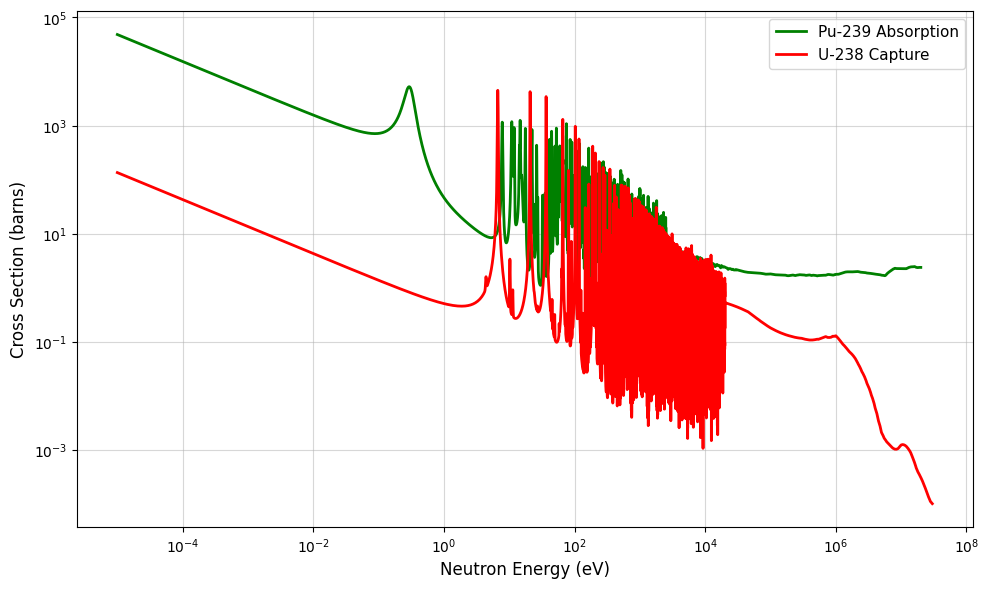
\includegraphics[width=0.75\linewidth]{figs/breed_burn_xs.png}
    \caption{Neutron cross sections for $^{238}$U radiative capture (breeding) and $^{239}$Pu absorption (burning) as functions of energy, evaluated from ENDF/B-VIII.0 at 900\,K \cite{Brown2018ENDF/B-VIII.0:Data}. In the thermal range, $\sigma_\text{a,Pu239}$ exceeds $\sigma_{(n,\gamma),\text{U238}}$ by two to three orders of magnitude, establishing the physical basis for the LBR's thermal spectrum strategy.}
    \label{fig:breed-burn-xs}
\end{figure}

% ============================================================
\subsection{Preliminary Neutronics Scoping (D. Frank)}
\label{sec:scoping}
% ============================================================

The cross-section analysis establishes the need for a highly thermalized spectrum but does not by itself determine the moderator material or lattice geometry. A series of preliminary scoping calculations was performed on an infinite lattice model to identify a viable design point before proceeding to higher-fidelity analysis.

\subsubsection{Moderator and Lattice Pitch: Infinite Lattice Study}

An infinite lattice model was constructed in OpenMC, selected for its seamless integration with Python scripting, which facilitated the parametric sweep over moderator types and lattice pitches. Fuel compositions were drawn from radiochemical assay data for a spent fuel rod at Three Mile Island Unit 1 (TMI-1|NJ05|H6|C2B), with a discharge burnup of 52.6\,GWd/tHM and an initial enrichment of 4.01\,wt\%. This sample, among the highest-burnup specimens in the SFCOMPO-2.0 database \cite{Michel-Sendis2017SFCOMPO-2.0:Data}, was selected as a conservative baseline on the basis that highly depleted fuel maximizes the challenge to criticality (see Appendix \ref{sec:app_fuel-ref}, Table \ref{tab:tmi1_rod_characteristics} for isotopic profile). Three moderator candidates were evaluated --- light water (H$_2$O), heavy water (D$_2$O), and helium --- over a lattice pitch range of 1.5 to 15\,cm.

Figure~\ref{fig:kinf-pitch} shows $k_\infty$ at startup as a function of lattice pitch for each moderator. Light water and helium fail to sustain criticality at any pitch for fuel of this burnup. Heavy water is the only candidate that achieves $k_\infty > 1$, owing to its low thermal neutron absorption cross section ($\sigma_\text{a,D2O} \approx 0.001$\,b) compared to light water ($\sigma_\text{a,H2O} \approx 0.33$\,b), which preserves neutron economy in a fuel-poor lattice. The D$_2$O system reaches $k_\infty > 1$ for pitches above $\sim$3\,cm and plateaus near 1.27 for pitches of 6 to 15\,cm.

\begin{figure}[H]
    \centering
    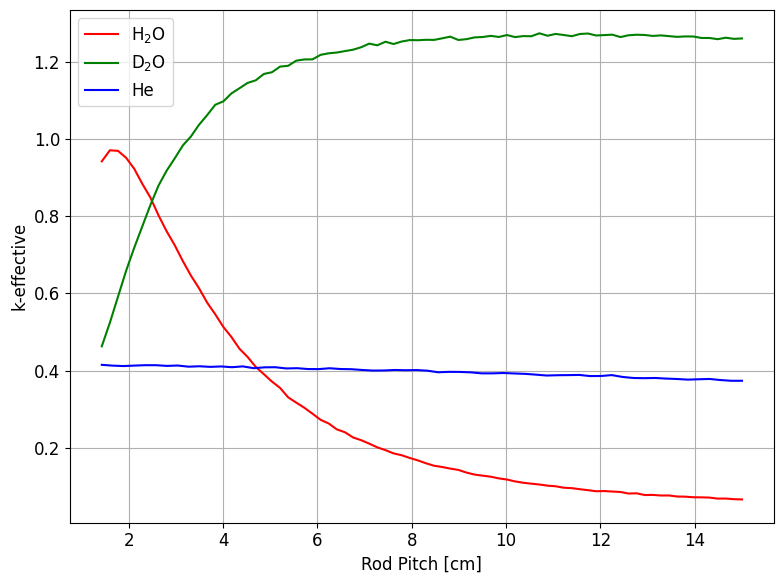
\includegraphics[width=0.73\linewidth]{figs/KinfVsPitch.png}
    \caption{Infinite multiplication factor $k_\infty$ at startup versus lattice pitch for H$_2$O, D$_2$O, and He moderation, using the TMI-1 spent fuel composition (52.6\,GWd/tHM). Light water and helium fail to achieve criticality at any pitch; D$_2$O reaches $k_\infty > 1$ for pitches above $\sim$3\,cm and plateaus near 1.27 for pitches of 6 to 15\,cm.}
    \label{fig:kinf-pitch}
\end{figure}

The reaction rates for $^{239}$Pu absorption (burning) and $^{238}$U capture (breeding) as functions of lattice pitch are compared in Figure~\ref{fig:breed-burn-rr}. Only the D$_2$O system satisfies the burning-over-breeding condition ($\lambda_3 > \lambda_2$) established in Section~\ref{sec:transmutation-kinetics}, and does so across a broad range of pitches, confirming heavy water as the only viable moderator for net plutonium reduction.

\begin{figure}[H]
    \centering
    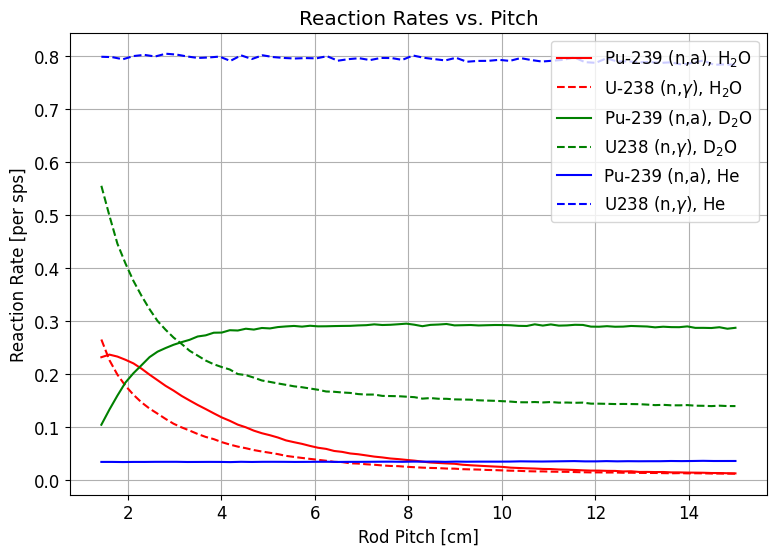
\includegraphics[width=0.73\linewidth]{figs/RRvsPitch.png}
    \caption{Normalized $^{239}$Pu absorption (burning) and $^{238}$U capture (breeding) reaction rates versus lattice pitch for H$_2$O and D$_2$O moderation. Heavy water uniquely sustains a configuration in which the burning rate exceeds the breeding rate ($\lambda_3 > \lambda_2$) over a broad pitch range, confirming D$_2$O as the only viable moderator for net plutonium reduction.}
    \label{fig:breed-burn-rr}
\end{figure}

A lattice pitch of 6\,cm was selected as the baseline design point, balancing three competing requirements:
\begin{enumerate}
    \item Sufficient spectrum thermalization to maintain $\lambda_3/\lambda_2 > 1$ (Objective~1: plutonium burning).
    \item Adequate initial excess reactivity ($k_\infty \approx 1.22$) to sustain criticality throughout the fuel cycle (Objective~2).
    \item Small enough to allow for sufficient heat removal (Objective~3), discussed further in \S~\ref{sec:th-scoping}. %FIND THIS
\end{enumerate}

\subsubsection{Zero-Dimensional Depletion Analysis}

Having established D$_2$O moderation at a 6\,cm pitch as the design point, a zero-dimensional (0-D) depletion analysis was performed to assess achievable burnup, plutonium burndown, and isotopic quality evolution under continuous irradiation at constant power. A specific power of 30\,W/gHM was assumed, consistent with typical PWR operation, yielding a total heavy metal inventory of approximately 67\,tonnes at 2\,GW$_\text{th}$ across $\sim$19,400 fuel rods.

\paragraph{Burnup Performance.}
Objective~2 requires $k_\text{eff} \geq 1$ through an accumulated discharge burnup of $\geq$60\,GWd/tHM. The 0-D model uses the TMI-1 C2B spent fuel composition (see App.~\ref{sec:app_fuel-ref}), which enters the LBR at 52.6\,GWd/tHM. The NRC regulatory ceiling of 62\,GWd/tHM therefore leaves 9.4\,GWd/tHM of available margin before the fuel must be discharged regardless of its reactivity state.

As shown in Figure~\ref{fig:kinf-burn}, $k_\infty \geq 1$ is maintained through an additional 9.0\,GWd/tHM of irradiation, bringing the total accumulated burnup to $\sim$61.6\,GWd/tHM --- within 0.4\,GWd/tHM of the regulatory ceiling and exceeding the 60\,GWd/tHM design objective. The initial excess reactivity ($k_\infty = 1.22$) would be managed in the finite reactor through soluble boron, control rods, or burnable poisons.

\begin{figure}[H]
    \centering
    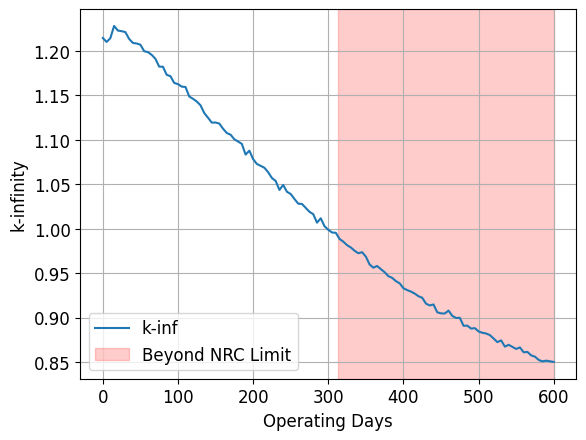
\includegraphics[width=0.8\linewidth]{figs/kinfVsBurn.png}
    \caption{Infinite multiplication factor $k_\infty$ versus accumulated burnup at 30\,W/gHM for the D$_2$O / 6\,cm pitch infinite lattice, starting from the TMI-1 C2B composition at 52.6\,GWd/tHM. Criticality is maintained through an additional 9.0\,GWd/tHM, reaching a total of $\sim$61.6\,GWd/tHM and exceeding the 60\,GWd/tHM design objective. The shaded region indicates operation beyond the NRC regulatory burnup ceiling of 62\,GWd/tHM.}
    \label{fig:kinf-burn}
\end{figure}

\paragraph{Fissile Inventory Evolution.}
The evolution of key fissile isotopes is shown in Figure~\ref{fig:conc-burn}. Over the 9.0\,GWd/tHM LBR irradiation, $^{235}$U depletes from 0.74\,wt\% to 0.30\,wt\% (a 59\% reduction), while $^{239}$Pu depletes from 0.59\,wt\% to 0.39\,wt\% (a 34\% reduction). Total plutonium decreases from 1.26\,wt\% to 0.99\,wt\%, a 21.5\% reduction that exceeds the 20\% design target. Continuous breeding from $^{238}$U partially replenishes the $^{239}$Pu inventory, consistent with the $\lambda_3/\lambda_2 > 1$ condition established earlier: net destruction proceeds, but is partially offset by in-situ production. Integrating over the full core, this corresponds to the destruction of approximately 16\,kg of plutonium per tonne of heavy metal processed, or $\sim$1\,070\,kg total.

\begin{figure}[H]
    \centering
    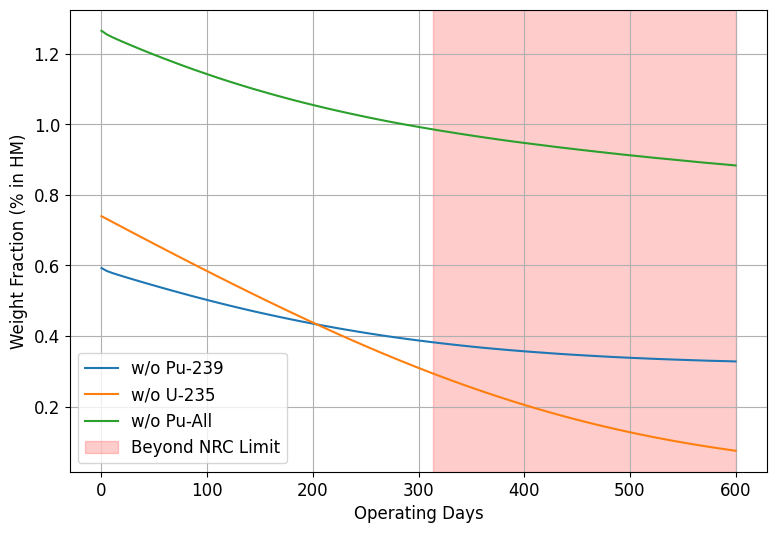
\includegraphics[width=0.8\linewidth]{figs/concVsBurn.png}
    \caption{Fissile isotope weight fractions versus operating time. $^{235}$U depletes from 0.74\% to 0.30\% (59\% reduction) while $^{239}$Pu depletes from 0.59\% to 0.39\% (34\% reduction). Total plutonium decreases from 1.26\% to 0.99\%, a 21.5\% reduction exceeding the 20\% design target. Continuous breeding from $^{238}$U partially replenishes the $^{239}$Pu inventory, consistent with the $\lambda_3/\lambda_2 > 1$ condition.}
    \label{fig:conc-burn}
\end{figure}

\paragraph{Plutonium Isotopic Quality Degradation.}
Beyond total mass reduction, the isotopic composition of the remaining plutonium evolves in a direction that degrades its weapons utility. As shown in Figure~\ref{fig:attractiveness}, the fissile isotopes $^{239}$Pu and $^{241}$Pu decrease over the cycle while $^{238}$Pu, $^{240}$Pu, and $^{242}$Pu accumulate. The relative $^{239}$Pu fraction decreases by 24.7\%, while the $^{240}$Pu fraction --- which carries a high spontaneous fission rate --- increases by 30.0\% relative to total plutonium. This isotopic shift simultaneously reduces net fissile content and increases self-heating and neutron emission rates, degrading the material's utility for weapons applications even if it were chemically separated.

\begin{figure}[H]
    \centering
    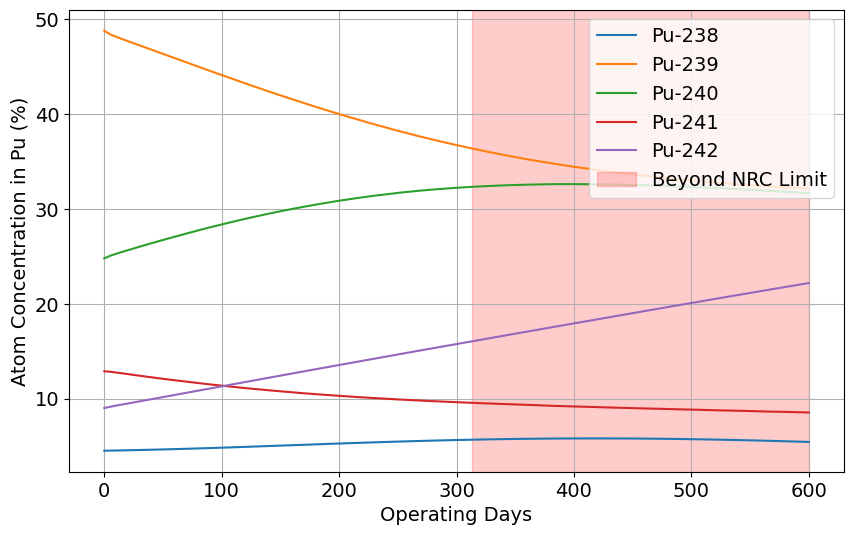
\includegraphics[width=0.8\linewidth]{figs/attractiveness.png}
    \caption{Plutonium isotopic composition versus operating time. The fissile isotopes $^{239}$Pu and $^{241}$Pu decrease while $^{238}$Pu, $^{240}$Pu, and $^{242}$Pu accumulate, progressively degrading weapons attractiveness through elevated decay heat, higher spontaneous fission rates, and a reduced fissile fraction.}
    \label{fig:attractiveness}
\end{figure}

\paragraph{0-D Scoping Summary.}
The 0-D infinite lattice analysis confirms that the two neutronics-driven design objectives are achievable at the scoping level:
\begin{itemize}
    \item \textbf{Objective 1 --- Plutonium reduction}: $^{239}$Pu decreases by 34\% and total Pu by 21.5\%, both exceeding the $\geq$20\% target; $^{240}$Pu fraction increases by 30\%, degrading weapons attractiveness.
    \item \textbf{Objective 2 --- Sustained criticality}: $k_\infty \geq 1$ through 9.0\,GWd/tHM of additional irradiation, reaching a total accumulated burnup of $\sim$61.6\,GWd/tHM and exceeding the $\geq$60\,GWd/tHM target.
\end{itemize}

These results assume spatially uniform depletion in an ideal infinite lattice. Several phenomena lie outside the scope of this approximation and require higher-fidelity treatment before the design can be considered credible:

\begin{enumerate}
    \item \textbf{Non-uniform spent fuel burnup.} Real PWR assemblies discharge with a spatially varying burnup profile: rod extremities retain substantially more fissile material than the axial midplane. A 0-D model assigns a single composition to the entire fuel volume and therefore cannot represent this variation, meaning the isotopic starting conditions for the LBR differ significantly from those of a single-composition infinite lattice.
    \item \textbf{Isotopic validation.} The 0-D model uses a single measured composition from SFCOMPO-2.0, but a full assembly model requires spatially varying fuel compositions across the rod length. These must be generated by a depletion code and subsequently validated against the remaining measured compositions in SFCOMPO-2.0 before they can be trusted as LBR fuel inputs.
    \item \textbf{Spectral coupling between moderator and fuel.} The spatial distribution of D$_2$O and fuel in a real assembly modifies both the effective moderation ratio and the flux-weighted cross sections relative to the infinite lattice assumption, altering the predicted reaction rate balance.
    \item \textbf{Axial power redistribution.} The non-uniform fissile profile drives an axially peaked power distribution that is invisible to 0-D models but directly affects cycle length, thermal margins, and fuel utilization efficiency.
\end{enumerate}

These limitations define the scope of the detailed Monte Carlo analyses presented in \S~\ref{sec:neutronics}: (i)~a Serpent~2 depletion model of Assembly NJ05YU from TMI-1 is benchmarked against measured isotopic data to validate the spent fuel compositions; (ii)~a full-assembly Serpent lattice model replaces the infinite lattice approximation for moderator and pitch selection; and (iii)~an iterative design study identifies and optimizes a power-redistribution strategy to address the axial burnup non-uniformity that the scoping analysis could not resolve.

\subsection{Preliminary Thermal-Hydraulic Scoping (S. Yeatts)}
\label{sec:th-scoping}


\clearpage

% ===================================================================
% NEUTRONICS
% ===================================================================
\section{Neutronics Design and Analysis (D. Frank)}
\label{sec:neutronics}
% ============================================================
%  NEUTRONICS ANALYSES
% ============================================================

Neutronics analyses were performed using the Serpent~2 Monte Carlo neutron and photon transport code \cite{Leppanen2025Status2024}. Serpent was selected over deterministic alternatives for its advanced capabilities in coupled burnup calculations, including: burnup-dependent geometry evolution, detailed chemical and radiological toxicity tracking, flexible depletion zone subdivision, universe nesting and reflective symmetry options, efficient parallel processing via domain decomposition, robust material definition transfers between models via binary restart files, fine control of numerical solvers (CRAM, TTA, and substep methods), and a comprehensive Python-based output-parsing library (SerpentTools) \cite{Johnson2020SerpentTools:Serpent}. These features are particularly well-suited to the multi-physics demands of the Lead-cooled Breeder Reactor (LBR) design workflow, where spent fuel material compositions must be reliably transported across successive simulation stages.

% ============================================================
\subsection{Spent Fuel Characterization: TMI-1 Benchmark}
% ============================================================

Spent fuel material definitions were generated using an axially-resolved model of a fuel assembly from Three Mile Island Unit~1 (TMI-1). TMI-1 was selected as the benchmark case due to the availability of well-documented, spatially resolved isotopic and burnup distribution data for the assembly NJ05YU, which enables rigorous verification and validation (V\&V) of the depletion methodology prior to application in the LBR design iteration \cite{Wolf2000AnalysisReport}. The Serpent model geometry was constructed on the basis of a 1998 MCNP reference calculation \cite{Wright1998CRCI.}.

The assembly geometry, shown in Figure~\ref{fig:tmi_geometry}, is discretized axially into a series of depletion zones to capture the spatially non-uniform burnup profile that results from flux gradients, control rod positioning, and coolant density variation along the rod length. Structural components — including upper and lower grid spacers, flanges, and flow distribution hardware — are explicitly modeled with region-specific material assignments. Key geometric and material parameters are summarized in Table~\ref{tab:figure_labels}.

\begin{figure}[H]
    \centering
    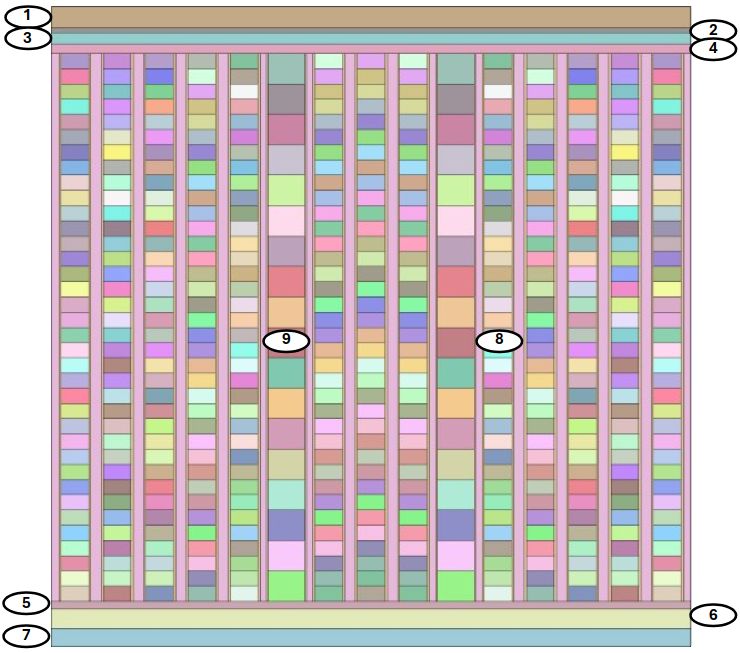
\includegraphics[width=0.65\linewidth]{figs/TMI_xz_plot.png}
    \caption{Axial cross-section of the TMI-1 fuel assembly Serpent geometry showing subdivided depletion zones. Structural components are labeled; axes are not to scale.}
    \label{fig:tmi_geometry}
\end{figure}

\begin{table}[H]
\centering
\caption{Labeled components of the TMI-1 fuel assembly geometry shown in Figure~\ref{fig:tmi_geometry}. Dimension $t$ denotes axial thickness; $d$, $L$, and $p$ denote diameter, active length, and rod pitch, respectively.}
\label{tab:figure_labels}
\renewcommand{\arraystretch}{1.4}
\begin{tabular}{c l l l}
\toprule
\textbf{Label} & \textbf{Component} & \textbf{Dimensions [cm]} & \textbf{Material} \\
\midrule
\ovalbox{1} & Upper Plenum   & $t = 14.14$ & SS-304 / borated water \\
\ovalbox{2} & Upper Flange   & $t = 3.18$  & SS-304 / borated water \\
\ovalbox{3} & Upper Grid     & $t = 7.62$  & SS-304 / borated water \\
\ovalbox{4} & Upper Pad      & $t = 5.08$  & SS-304 / borated water \\
\ovalbox{5} & Lower Pad      & $t = 5.08$  & SS-304 / borated water \\
\ovalbox{6} & Lower Grid     & $t = 12.70$ & SS-304 / borated water \\
\ovalbox{7} & Lower Plate    & $t = 12.22$ & SS-304 / borated water \\
\midrule
\ovalbox{8} & Fuel Rod &
\parbox[t]{3.4cm}{%
  $d_\text{pellet}   = 0.935$\\
  $d_\text{clad,in}  = 0.958$\\
  $d_\text{clad,out} = 1.092$\\
  $L_\text{active}   = 360.17$\\
  $p = 1.4427$
} &
\parbox[t]{3.4cm}{%
  UO\textsubscript{2} (4.0\,wt\%)\\
  Zircaloy-4 cladding\\
  He fill gas
} \\[1.8cm]
\ovalbox{9} & \parbox[t]{2.5cm}{Burnable\\Poison Rod} &
\parbox[t]{3.4cm}{%
  $d_\text{in}  = 1.265$\\
  $d_\text{out} = 1.346$\\
  $L_\text{active} = 360.17$
} &
\parbox[t]{3.4cm}{%
  Al\textsubscript{2}O\textsubscript{3}--B\textsubscript{4}C\\
  Zircaloy-4 cladding
} \\[1.0cm]
\bottomrule
\end{tabular}
\end{table}

% ============================================================
\subsubsection{Operating History and Depletion Solver Stability}
% ============================================================

Burnup simulations followed the irradiation history of Assembly NJ05YU as documented in \cite{Wolf2000AnalysisReport}, comprising: a 666-day first cycle with control rods fully inserted, a 36-day shutdown period, and a 692-day second cycle with control rods fully withdrawn. A constant assembly fission power of 14.508\,MW was maintained throughout all operating periods. The assembly-averaged discharge burnup is approximately 30\,GWd/MTU.

Two independent simulations of the operating history were performed, each using different numerical solver configurations — specifically, different depletion algorithms (CRAM-16 vs.\ a substep method) and timestep discretizations — in order to assess the sensitivity of isotopic predictions to solver parameters. As shown in Figure~\ref{fig:tmi-stability}, solver selection has a non-trivial effect on the predicted nuclide evolution, particularly for short-lived intermediaries and actinide chains that are sensitive to numerical stiffness. The stable configuration, characterized by finer substep divisions and higher-order CRAM, was adopted for all subsequent material generation.

\begin{figure}[H]
    \centering
    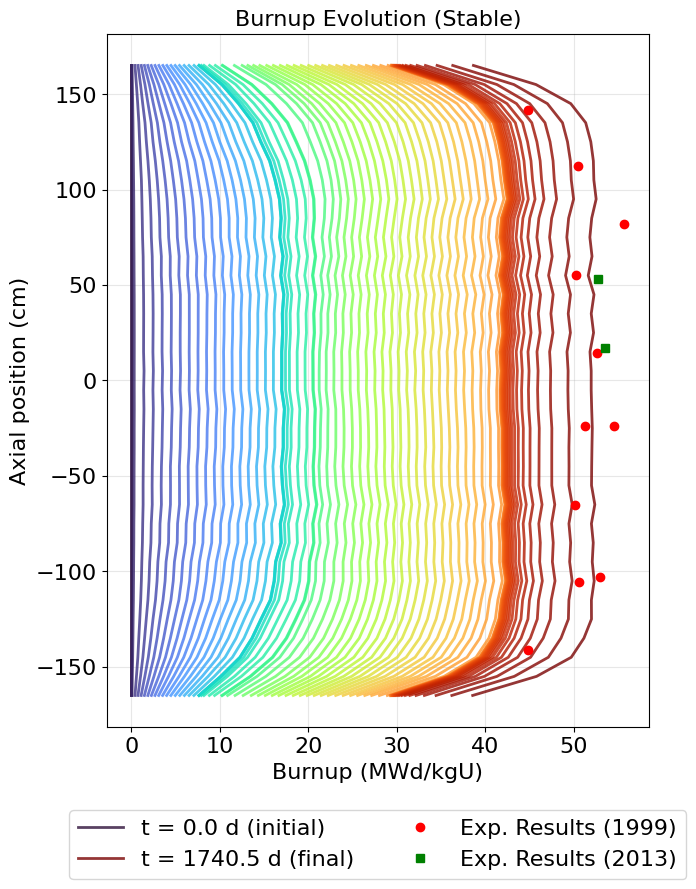
\includegraphics[width=0.48\linewidth]{figs/TMI_evol_stable.png}
    \hfill
    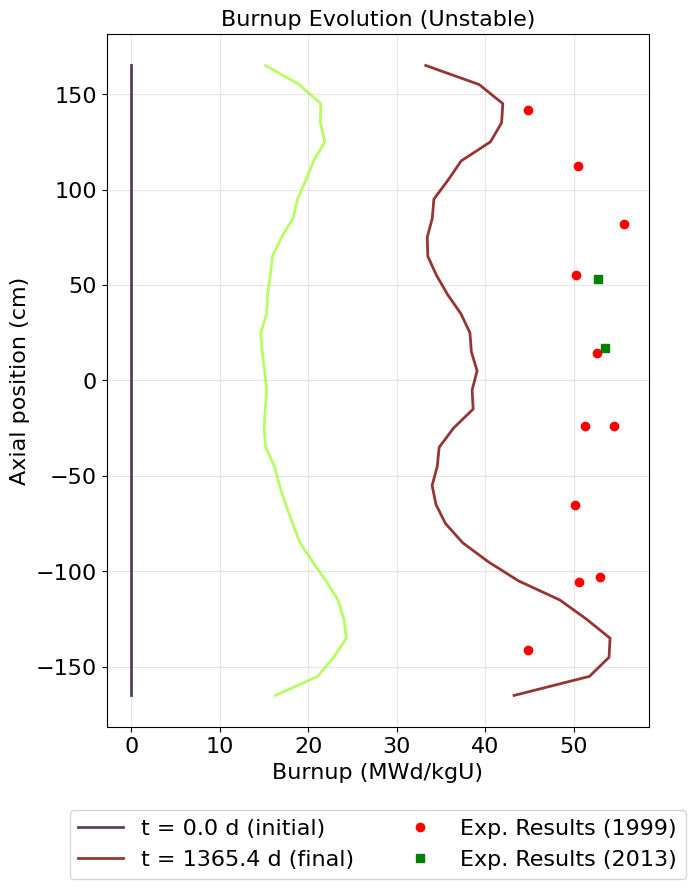
\includegraphics[width=0.48\linewidth]{figs/TMI_evol_unstable.png}
    \caption{Comparison of nuclide evolution computed with a numerically stable solver configuration (left) and an unstable configuration (right). Differences in predicted isotopic inventories highlight the sensitivity of burnup calculations to depletion timestep size and solver order, motivating careful solver selection prior to material extraction.}
    \label{fig:tmi-stability}
\end{figure}

% ============================================================
\subsubsection{Isotopic Validation Against Experimental Data}
% ============================================================

Spatial isotopic distributions predicted by the Serpent model were validated against radiochemical assay measurements of Assembly NJ05YU, originally reported in 1999 and subsequently re-evaluated in 2013 using updated nuclear data libraries \cite{Wolf2000AnalysisReport}. Validation focused on two key isotopes of interest: $^{235}$U, which serves as the primary fissile driver during irradiation, and $^{239}$Pu, whose in-situ production and consumption governs the breeding performance of the LBR concept.

The predicted axial distribution of $^{235}$U concentration is shown in Figure~\ref{fig:U235_evol_tmi} alongside experimental data at each reported irradiation stage. Simulation results fall within the $2\sigma$ uncertainty bounds of the measured data across the full active length, providing high confidence in the depletion model's treatment of $^{235}$U burnout.

\begin{figure}[H]
    \centering
    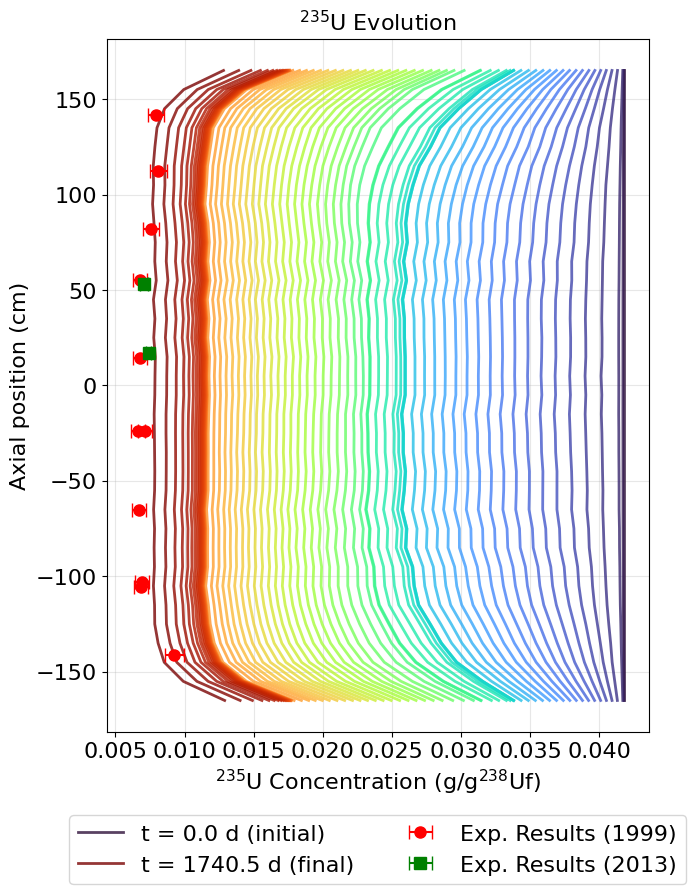
\includegraphics[width=0.65\linewidth]{U235_evol_tmi.png}
    \caption{Axial distribution of $^{235}$U concentration from initial loading through discharge, compared against radiochemical assay data. Simulation results (solid lines) fall within the $2\sigma$ experimental uncertainty bounds (shaded) at all irradiation stages, confirming the accuracy of the depletion model for the primary fissile species.}
    \label{fig:U235_evol_tmi}
\end{figure}

The predicted axial distribution of $^{239}$Pu is shown in Figure~\ref{fig:Pu239_evol_tmi}. Simulated results deviate considerably from the 1999 experimental dataset, but align closely with the 2013 re-evaluation, which incorporated revised cross-section libraries and updated decay data. This discrepancy is attributed to improvements in the nuclear data used for Pu production and capture reactions rather than deficiencies in the transport model itself. The agreement with the 2013 dataset provides confidence that the current simulation correctly captures plutonium buildup — a quantity of central importance to LBR breeding performance.

\begin{figure}[H]
    \centering
    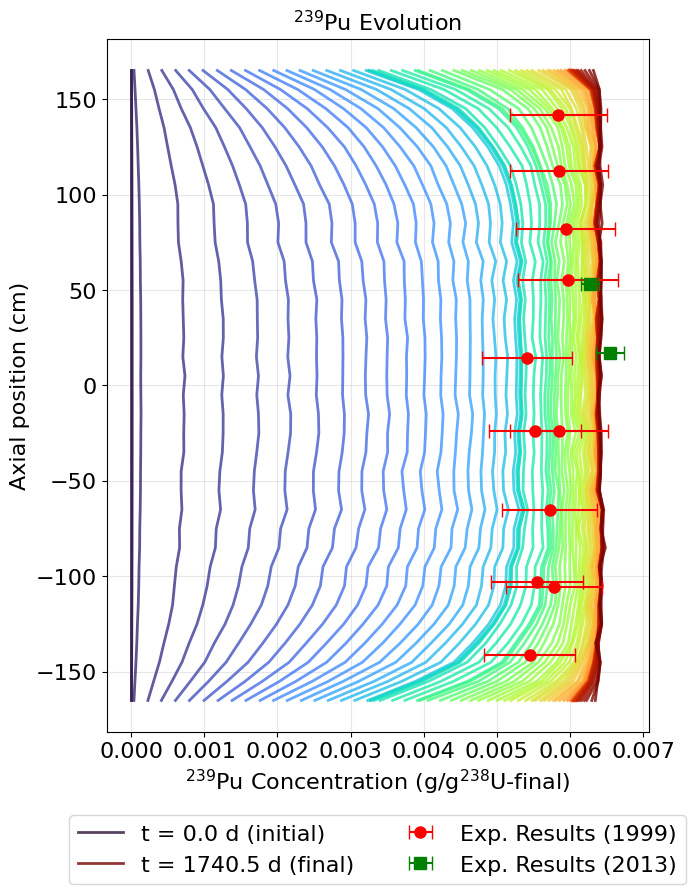
\includegraphics[width=0.65\linewidth]{Pu239_evol_tmi.png}
    \caption{Axial distribution of $^{239}$Pu concentration from initial loading through discharge, compared against the 1999 experimental assay and the 2013 re-evaluation. The improved agreement with the 2013 dataset is attributed to updated nuclear data libraries rather than model deficiencies, and provides confidence in predicted plutonium breeding behavior.}
    \label{fig:Pu239_evol_tmi}
\end{figure}

Taken together, the $^{235}$U and $^{239}$Pu validation results demonstrate that the TMI-1 depletion model accurately reproduces the isotopic composition of spent LWR fuel. The validated material definitions are subsequently transferred to the LBR lattice model via Serpent's binary restart file mechanism, eliminating interpolation error and preserving the full nuclide inventory for each axial depletion zone.

% ============================================================
\subsection{Moderator and Lattice Pitch Selection}
% ============================================================

The choice of moderator material and lattice pitch exerts the strongest influence on the neutron energy spectrum, initial reactivity, and the balance between fission and breeding reactions. Following the approach used in the preliminary 0-D scoping studies, a parametric sweep was conducted over a range of lattice pitches for each candidate moderator material. Candidate moderators considered in this study include light water (H$_2$O), heavy water (D$_2$O), and graphite. Spent fuel material definitions were transferred directly from the validated TMI-1 model via binary restart file, without fuel shuffling, ensuring that the lattice-level neutronics are evaluated using a physically consistent starting composition.

Two figures of merit (FOM) were used to guide pitch selection:
\begin{enumerate}
    \item \textbf{Initial excess reactivity} ($k_\infty - 1$): a measure of how much reactivity margin is available at the start of the critical cycle, which sets an upper bound on achievable cycle length.
    \item \textbf{Burn-to-breed ratio of $^{239}$Pu}: defined as the ratio of $^{239}$Pu consumed by fission to $^{239}$Pu produced by $^{238}$U capture, which quantifies the degree to which the assembly operates as a breeder versus a burner.
\end{enumerate}

The dependence of each FOM on lattice pitch and moderator selection is shown in Figures~\ref{fig:keff_sweep} and~\ref{fig:b2b_sweep}, respectively.

\begin{figure}[H]
    \centering
    \includegraphics[width=0.5\linewidth]{figs/absKeffLBR.png}
    \caption{Infinite multiplication factor $k_\infty$ as a function of lattice pitch for each candidate moderator material. Each curve reflects a constant spent fuel composition transferred from the TMI-1 benchmark model.}
    \label{fig:keff_sweep}
\end{figure}

\begin{figure}[H]
    \centering
    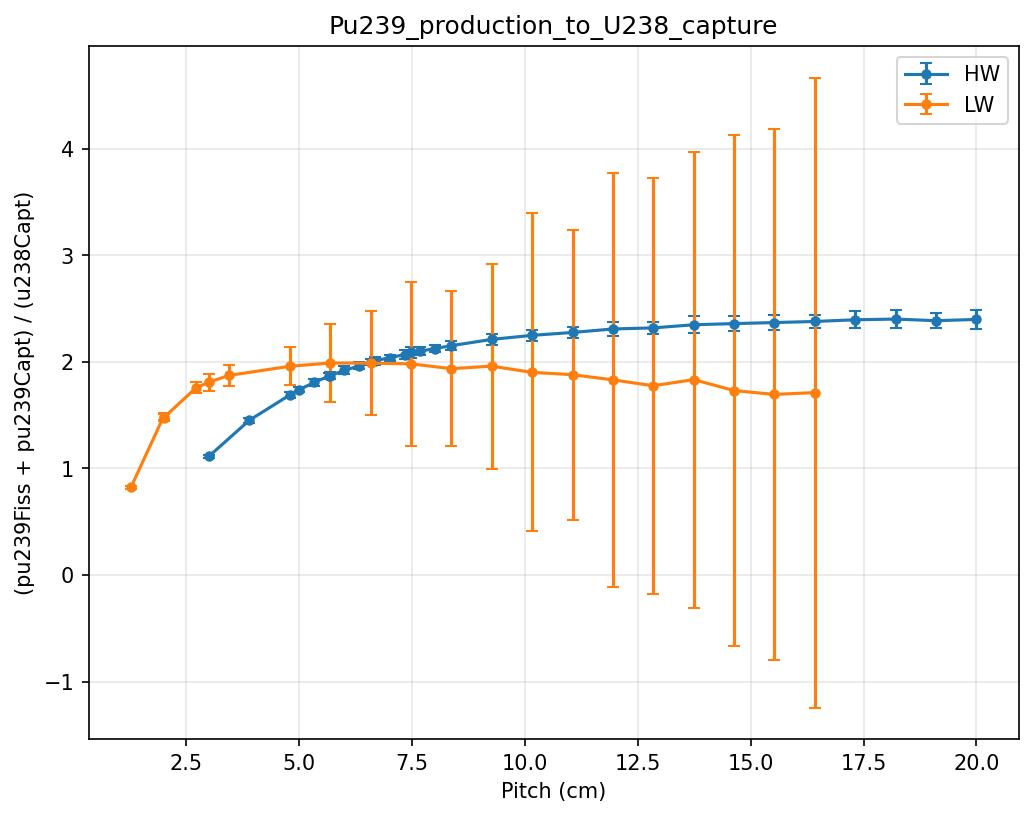
\includegraphics[width=0.5\linewidth]{figs/burnToBreedLBR.png}
    \caption{Burn-to-breed ratio of $^{239}$Pu as a function of lattice pitch for each candidate moderator. Values below unity indicate net plutonium production (breeding mode); values above unity indicate net consumption (burning mode).}
    \label{fig:b2b_sweep}
\end{figure}

Based on the results of the pitch sweep, a lattice pitch of 6\,cm with heavy water moderation was selected as the reference design point. This combination yields a sufficiently positive initial reactivity to support a meaningful critical cycle length while maintaining a burn-to-breed ratio below unity — indicating net in-situ plutonium production. This conclusion is consistent with the findings from the preliminary infinite-lattice scoping studies, providing cross-validation of the methodology across two levels of geometric fidelity.

% ============================================================
\subsection{Design Iteration}
% ============================================================

Examination of Figures~\ref{fig:U235_evol_tmi} and~\ref{fig:Pu239_evol_tmi} reveals a characteristic feature of PWR spent fuel: the upper and lower $\sim$50\,cm of each fuel rod retain a notably higher inventory of fissile material ($^{235}$U and $^{239}$Pu) relative to the axial midplane, due to flux depression by the adjacent structural hardware and control rod shadowing effects during the first irradiation cycle. In the baseline LBR configuration, these under-depleted end regions represent an underutilized fissile resource. Design iteration was therefore aimed at redistributing fission power toward the rod extremities to more efficiently exploit this inventory.

Design performance was assessed using two figures of merit evaluated at the end of the critical cycle:

\begin{enumerate}
    \item \textbf{Critical cycle length}: the duration over which $k_\text{eff} \geq 1$ is maintained, serving as a proxy for energy extraction and economic viability.
    \item \textbf{Coefficient of variation (CV) of fissile isotope distribution}: a dimensionless measure of axial uniformity in the fissile inventory at end-of-life, defined as:
\end{enumerate}

\begin{equation}
    \text{CV} = \frac{s}{\bar{w}} \times 100\%
    \label{eq:cv}
\end{equation}

\noindent where the sample mean $\bar{w}$ and standard deviation $s$ of the axial fissile weight fraction distribution are:

\begin{equation}
    \bar{w} = \frac{1}{N} \sum_{i=1}^{N} w_i, \qquad
    s = \sqrt{\frac{1}{N-1} \sum_{i=1}^{N} \left(w_i - \bar{w}\right)^2}
    \label{eq:cv_components}
\end{equation}

\noindent Here, $N$ is the number of equally sized axial depletion nodes, and $w_i$ is the total fissile weight percent (summed over $^{235}$U and $^{239}$Pu) at node $i$. A lower CV at end-of-life indicates a more axially uniform depletion profile, which is beneficial from both neutronics and fuel management perspectives, as it implies more complete utilization of the available fissile inventory and reduced peak-to-average power factors. Note that this metric is valid only for a uniform axial discretization in which each node $w_i$ represents an equal-length segment of the active fuel column.

Four design variants were evaluated, each representing a different strategy for redistributing fission power toward the rod extremities:

\paragraph{Baseline (Spent Fuel As-Is).}
In this configuration, the LBR assembly is loaded exclusively with spent PWR fuel rods in their as-discharged condition, with no additional devices or structural modifications. This case serves as the reference against which all modified designs are compared.

\paragraph{Beryllium End Reflectors.}
In this design, each fuel rod is fitted with beryllium ($^9$Be) axial reflector plugs in the upper and lower 70\,cm of the active zone, as illustrated in Figure~\ref{fig:be_caps_sketch}. Beryllium is an effective fast-neutron reflector and moderator due to its low neutron capture cross section and significant scattering cross section, and it is a neutron multiplier via the $^9$Be$(n,2n)$ reaction. The intent is to reflect neutrons that would otherwise stream axially out of the assembly back into the fissile end regions, thereby increasing the local thermal flux and enhancing fission rates in the less-depleted rod extremities.

\paragraph{Fresh Fuel Rods.}
In this design, every alternate lattice position is occupied by a fresh fuel rod. These rods have a graded enrichment profile: the central region (coinciding with the high-burnup zone of adjacent spent rods) is loaded with 5\,wt.\%\,UO$_2$, while the end regions are loaded with 10\,wt.\%\,UO$_2$ to compensate for the lower reactivity in the axial periphery and to promote peaked fission power at the rod extremities. This design introduces fresh fissile material as an active power-shaping tool.

\paragraph{Power Inverter Device.}
In this design, every alternate lattice position is occupied by a novel component designated the \textit{Power Inverter}. In the reference Power Inverter configuration, the upper and lower 70\,cm of each device contain 5\,wt.\%\,UO$_2$ fuel pins, while the central region is occupied by cerium dioxide (CeO$_2$, ceria) pins — all enclosed within a shared Zircaloy-4 cladding tube. The Power Inverter is designed to invert the axial power profile relative to the baseline: fission is concentrated in the end regions (co-located with the under-depleted extremities of the surrounding spent rods), while the central region contributes negligible fission power.

Ceria was selected as the central inert fill material for several reasons: (i) it is largely transparent to thermal neutrons due to its low absorption cross section, allowing the axial neutron flux to diffuse into the end fuel regions without being parasitically absorbed; (ii) it is chemically inert and thermally stable at LWR operating temperatures; and (iii) it shares closely matched thermo-mechanical properties with UO$_2$ — including crystal structure (fluorite), thermal conductivity, and coefficient of thermal expansion — which mitigates stress concentration and material compatibility concerns at the CeO$_2$/UO$_2$ interface.

The performance of each design variant against the two figures of merit is discussed in Section~\ref{sec:results}. % <-- update cross-ref as needed


\begin{figure}[H]
    \centering
    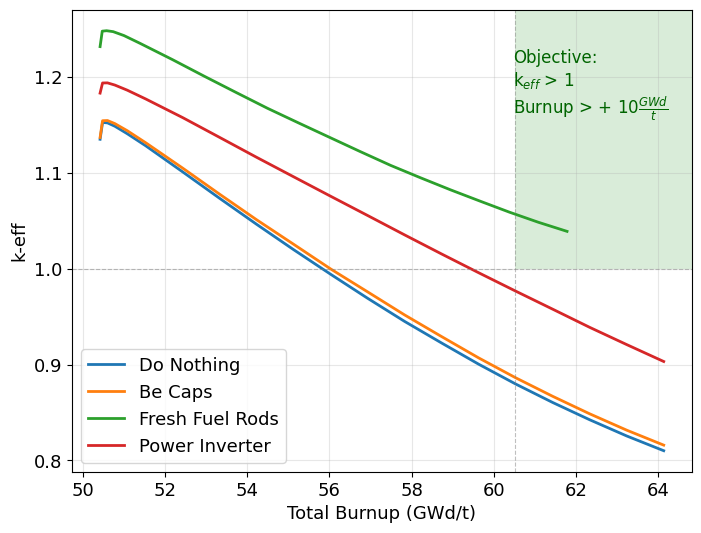
\includegraphics[width=0.75\linewidth]{figs/4-designs-keff.png}
    \caption{Enter Caption}
    \label{fig:placeholder}
\end{figure}

\begin{figure}[H]
    \centering
    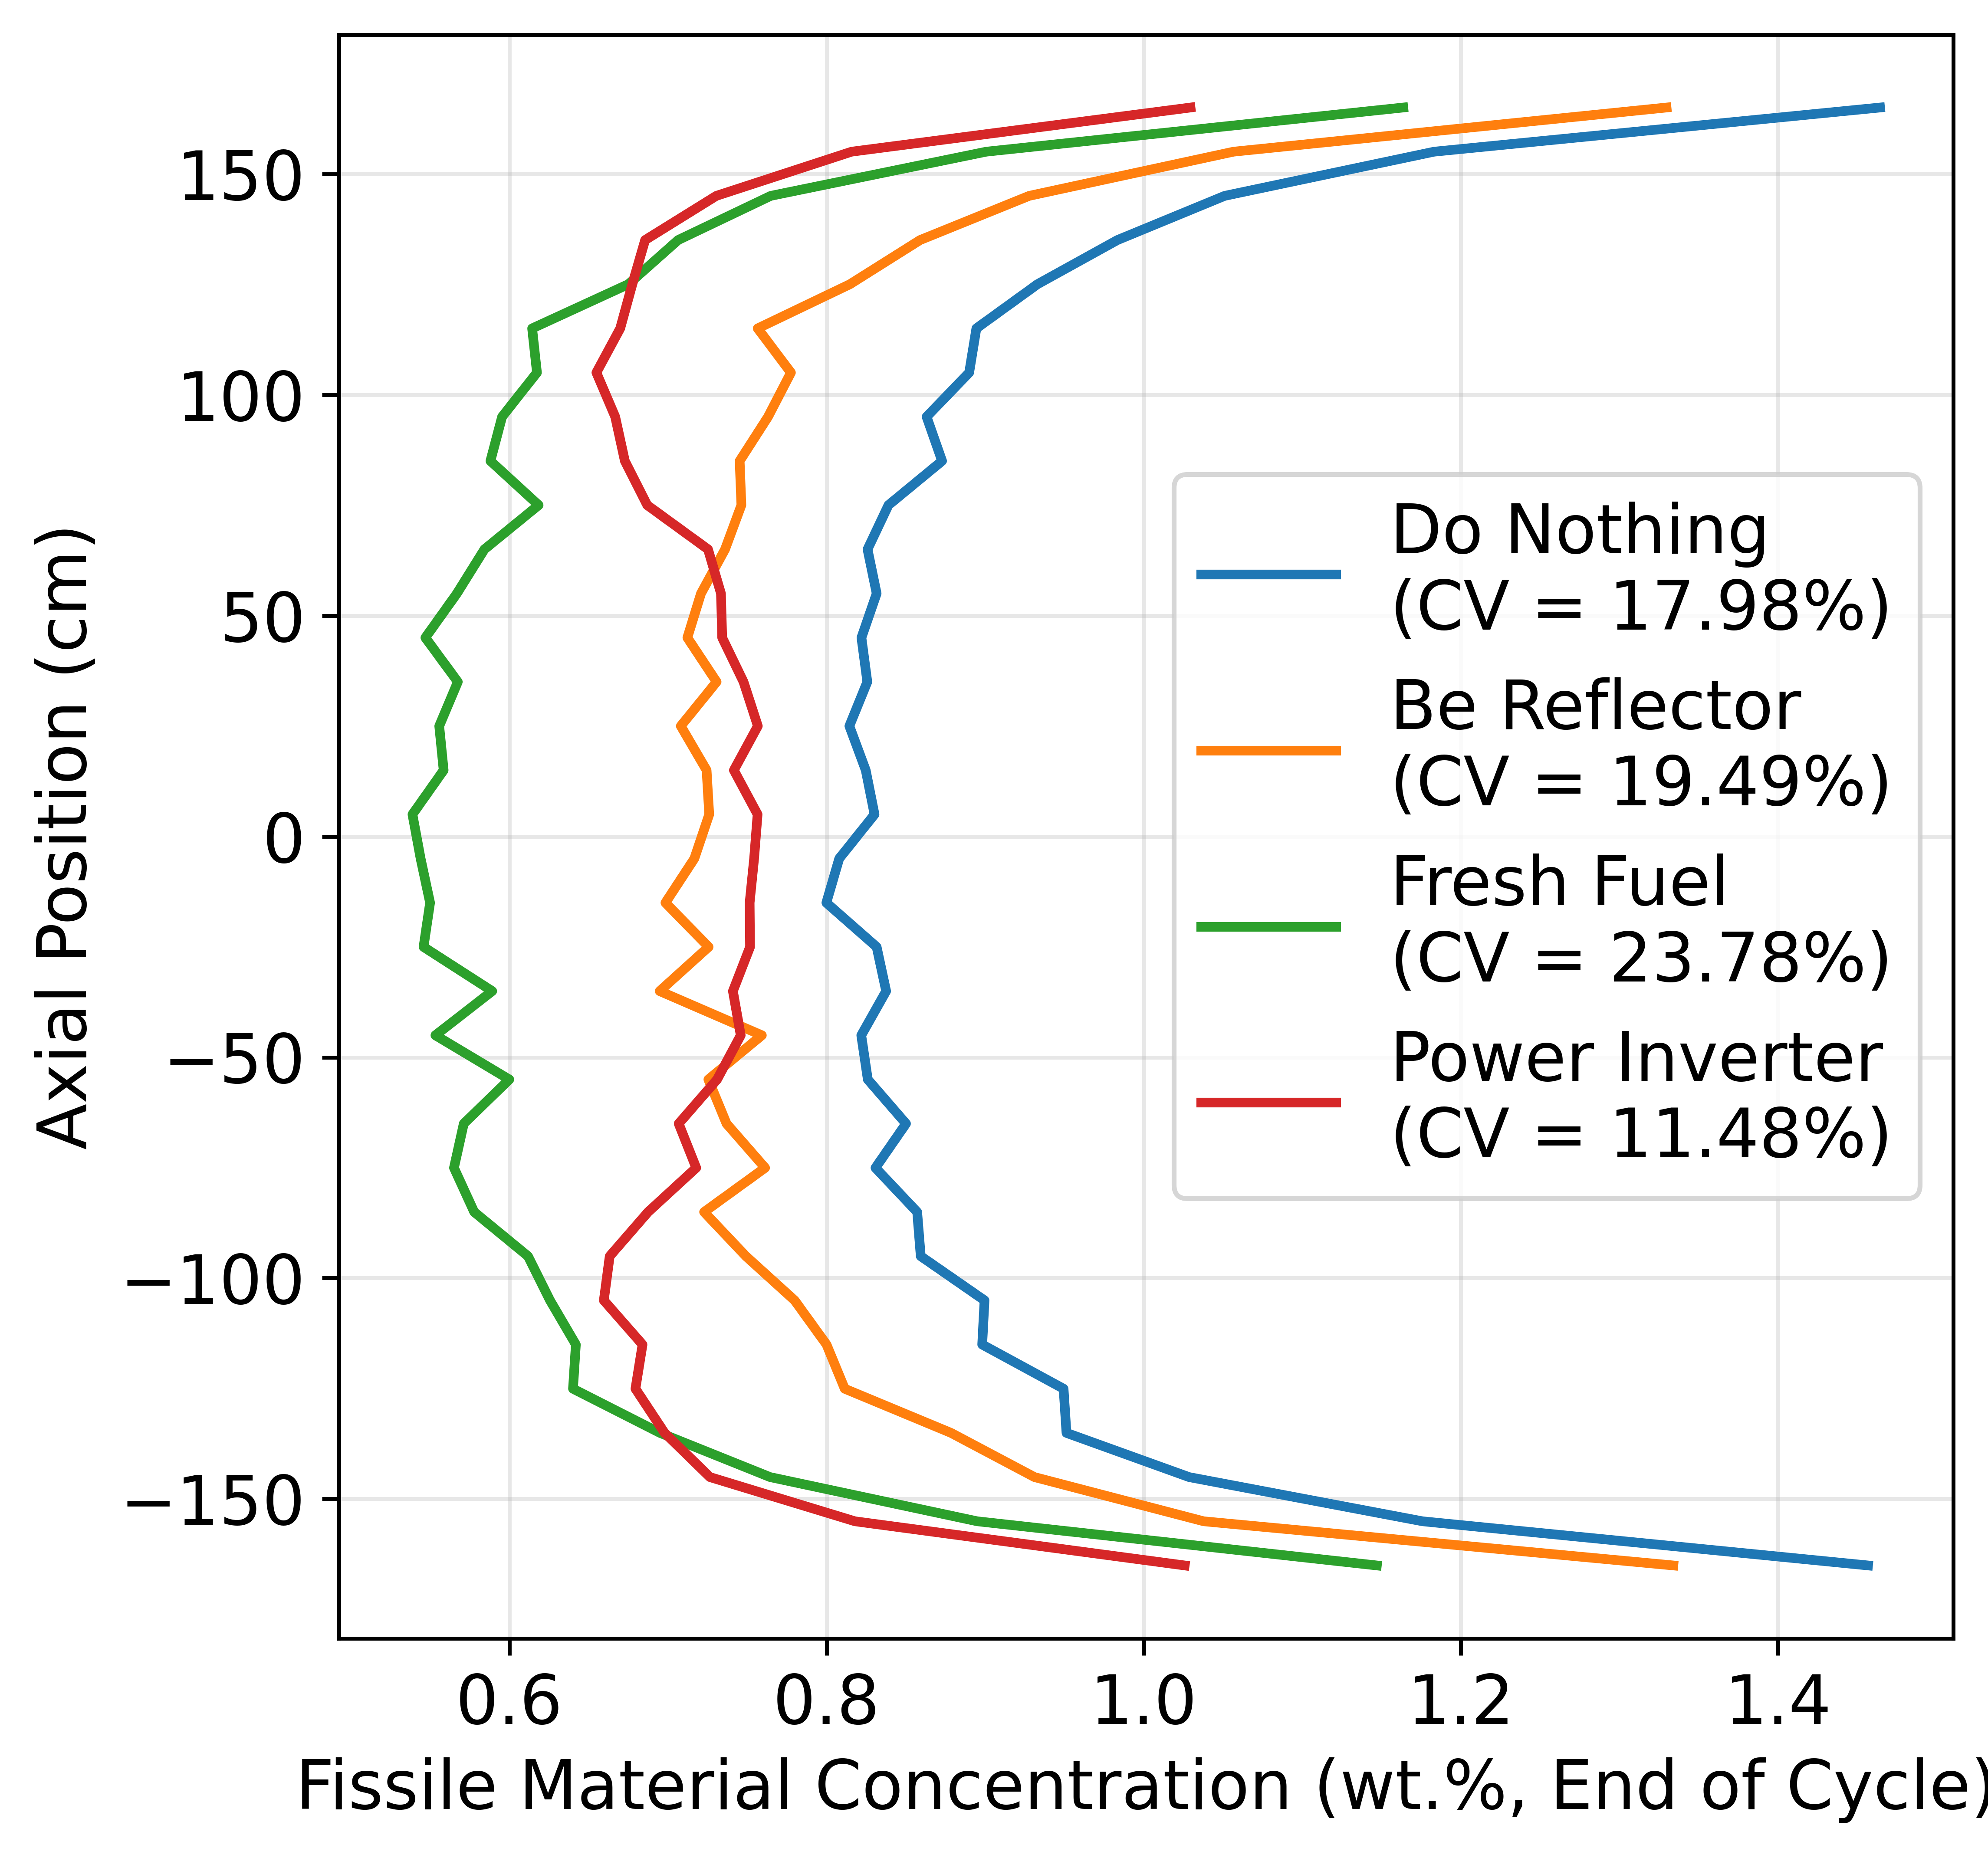
\includegraphics[width=0.75\linewidth]{figs/4-designs-fiss-dist.png}
    \caption{Enter Caption}
    \label{fig:placeholder}
\end{figure}

\newpage

\begin{figure}[H]
    \centering
    \begin{subfigure}[t]{0.48\linewidth}
        \centering
        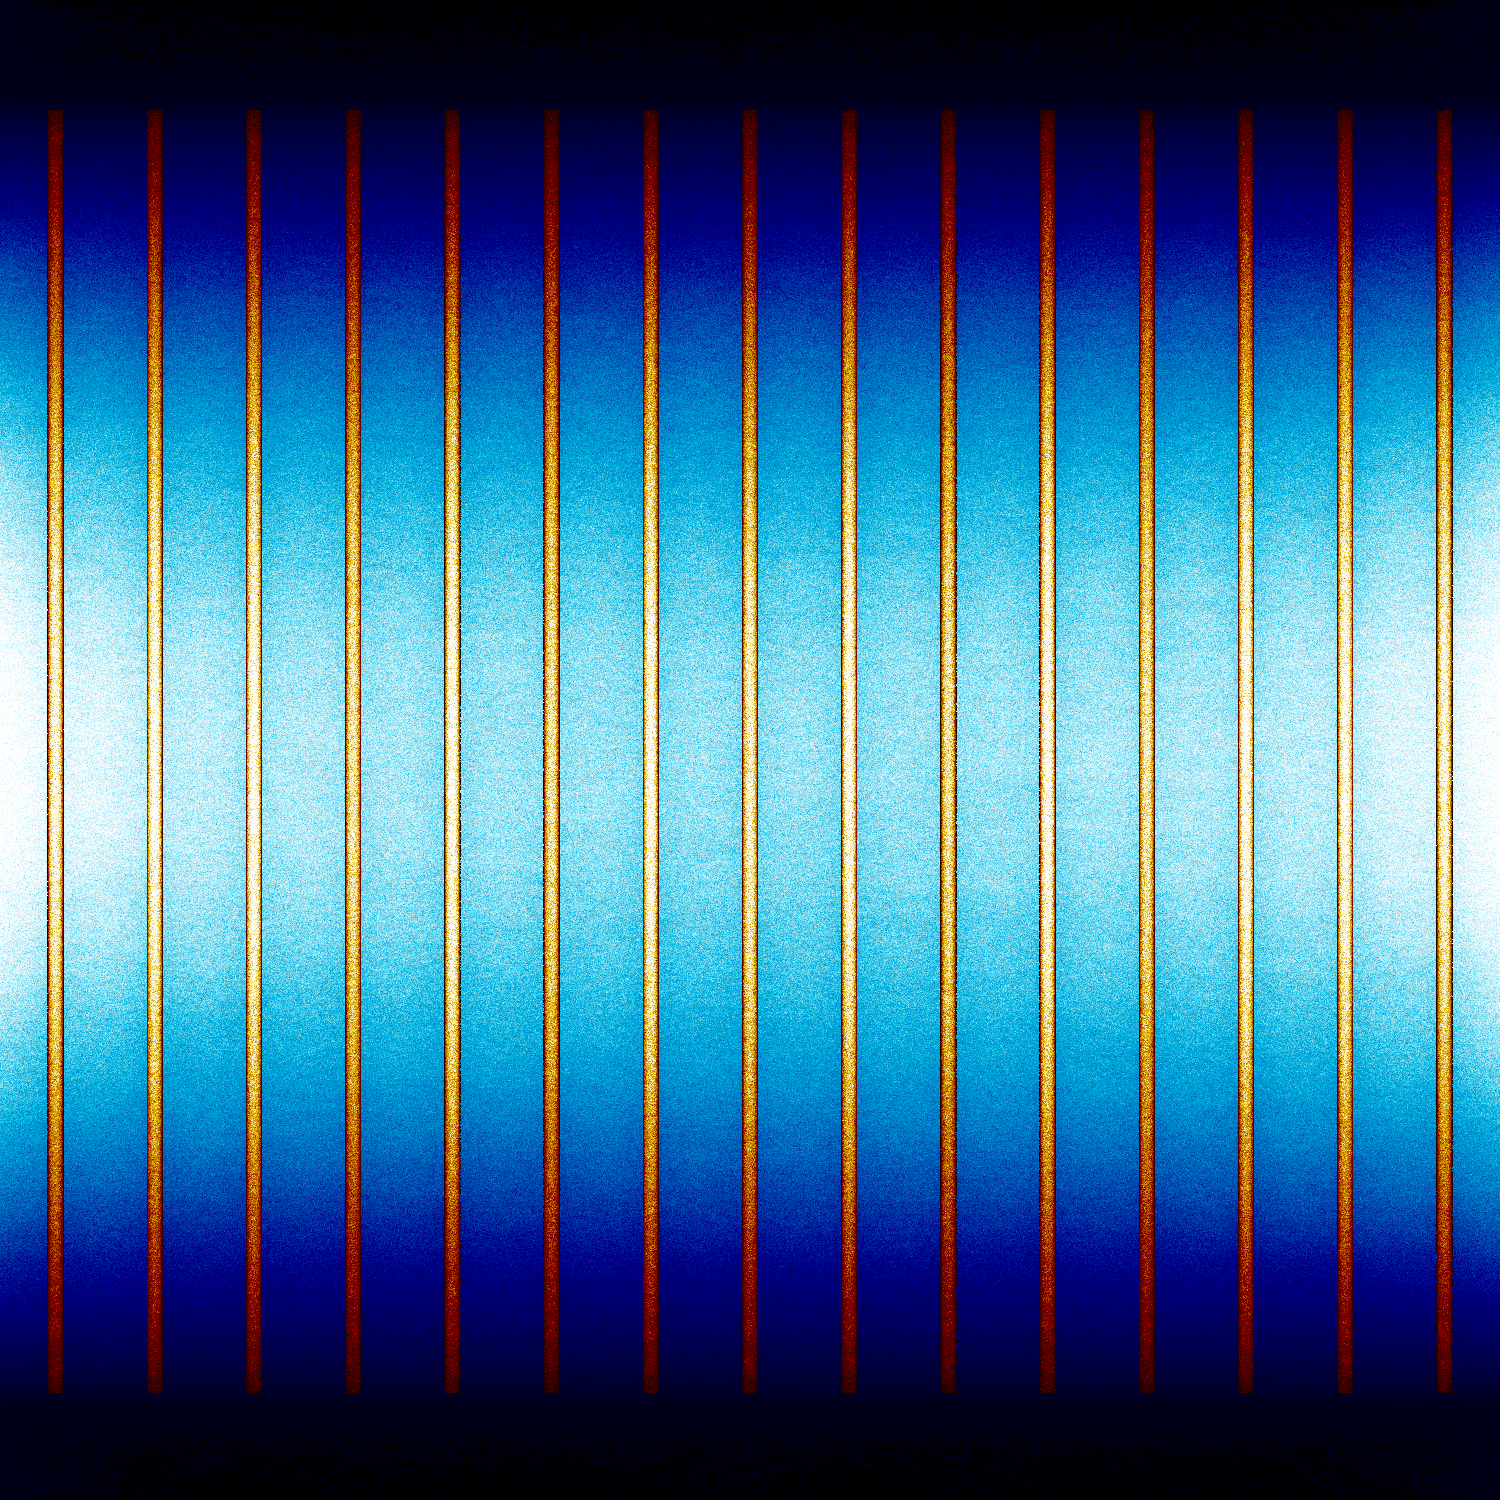
\includegraphics[width=\linewidth]{figs/powerdist-donothing.png}
        \caption{Baseline}
    \end{subfigure}
    \hfill
    \begin{subfigure}[t]{0.48\linewidth}
        \centering
        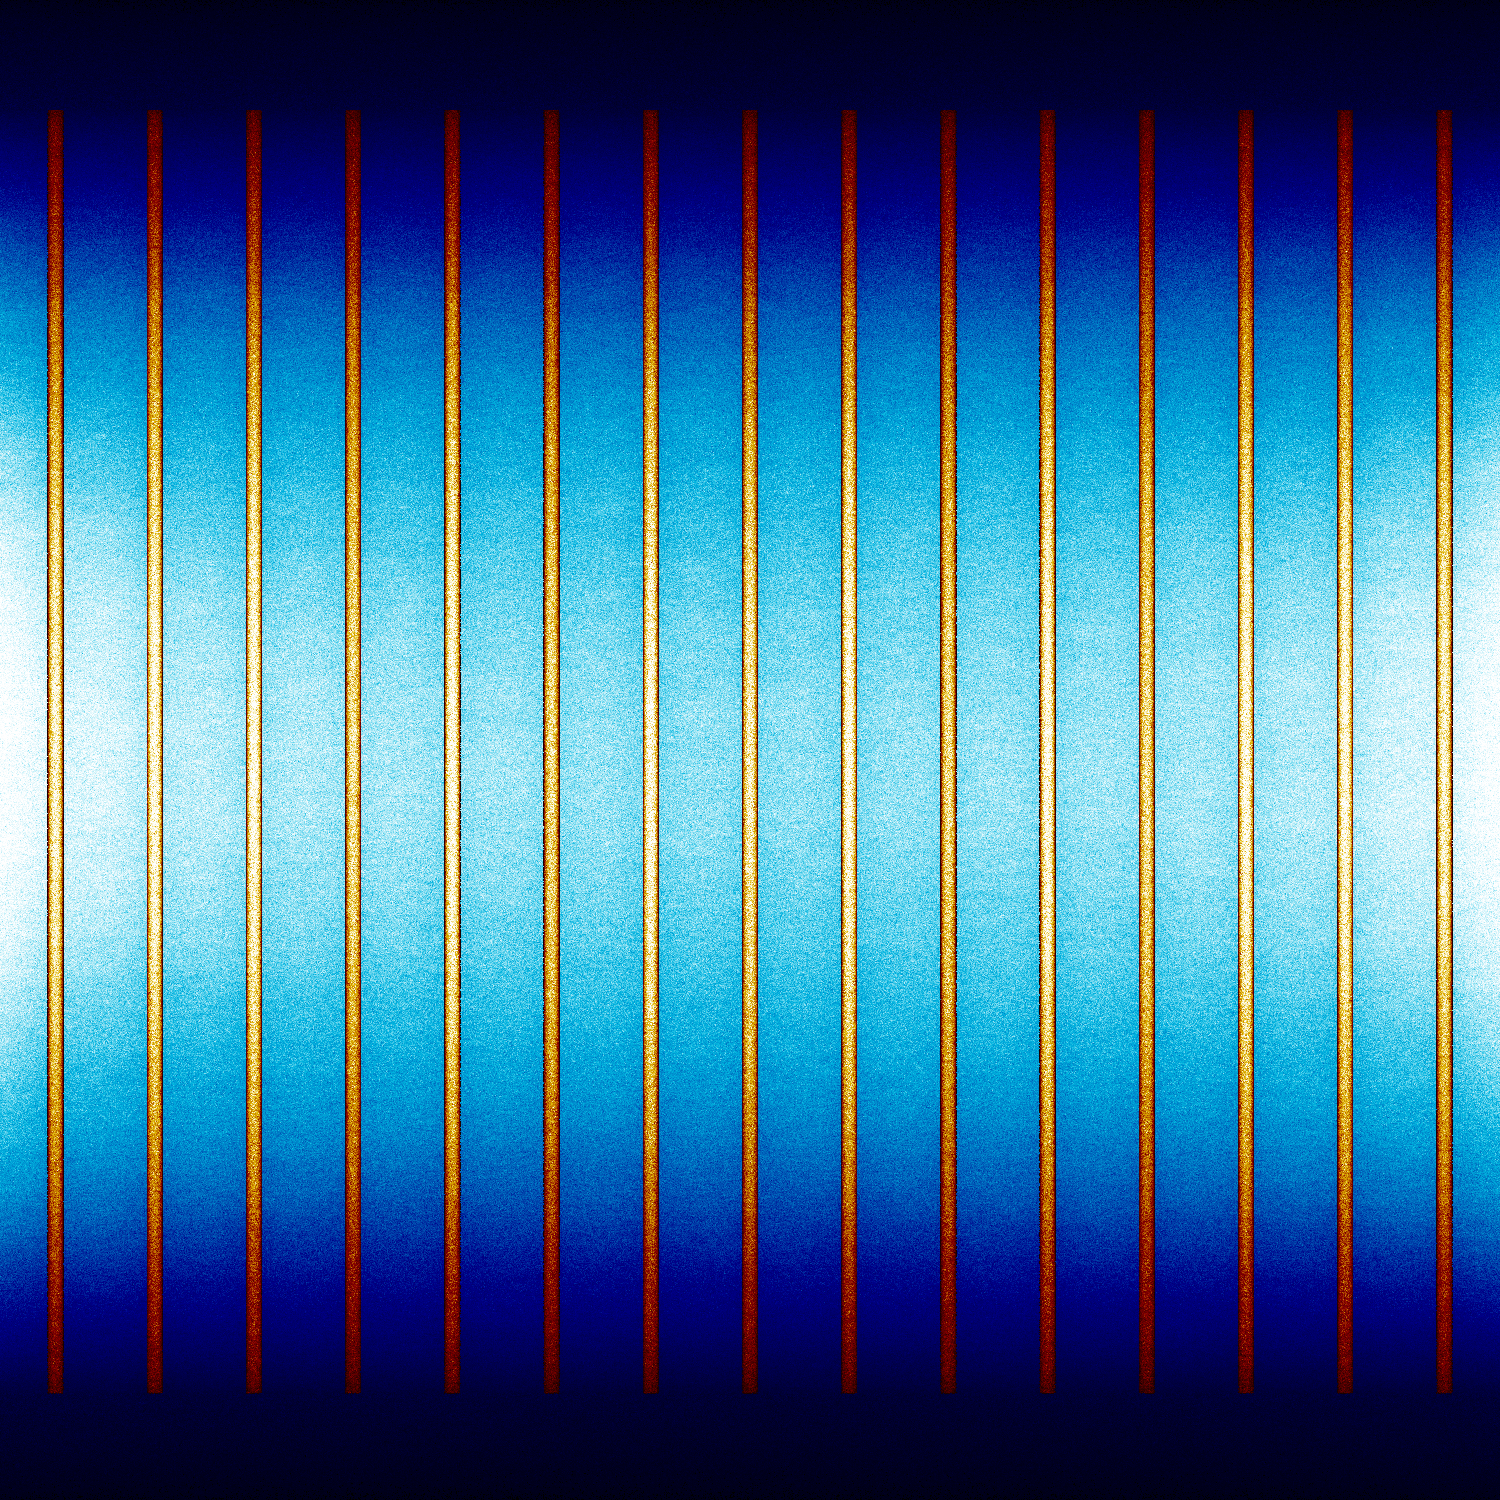
\includegraphics[width=\linewidth]{figs/powerdist-becaps.png}
        \caption{Beryllium End Reflectors}
    \end{subfigure}

    \medskip

    \begin{subfigure}[t]{0.48\linewidth}
        \centering
        
\includegraphics[width=\linewidth]{figs/powerdist-freshrods.png}
        \caption{Fresh Fuel Rods}
    \end{subfigure}
    \hfill
    \begin{subfigure}[t]{0.48\linewidth}
        \centering
        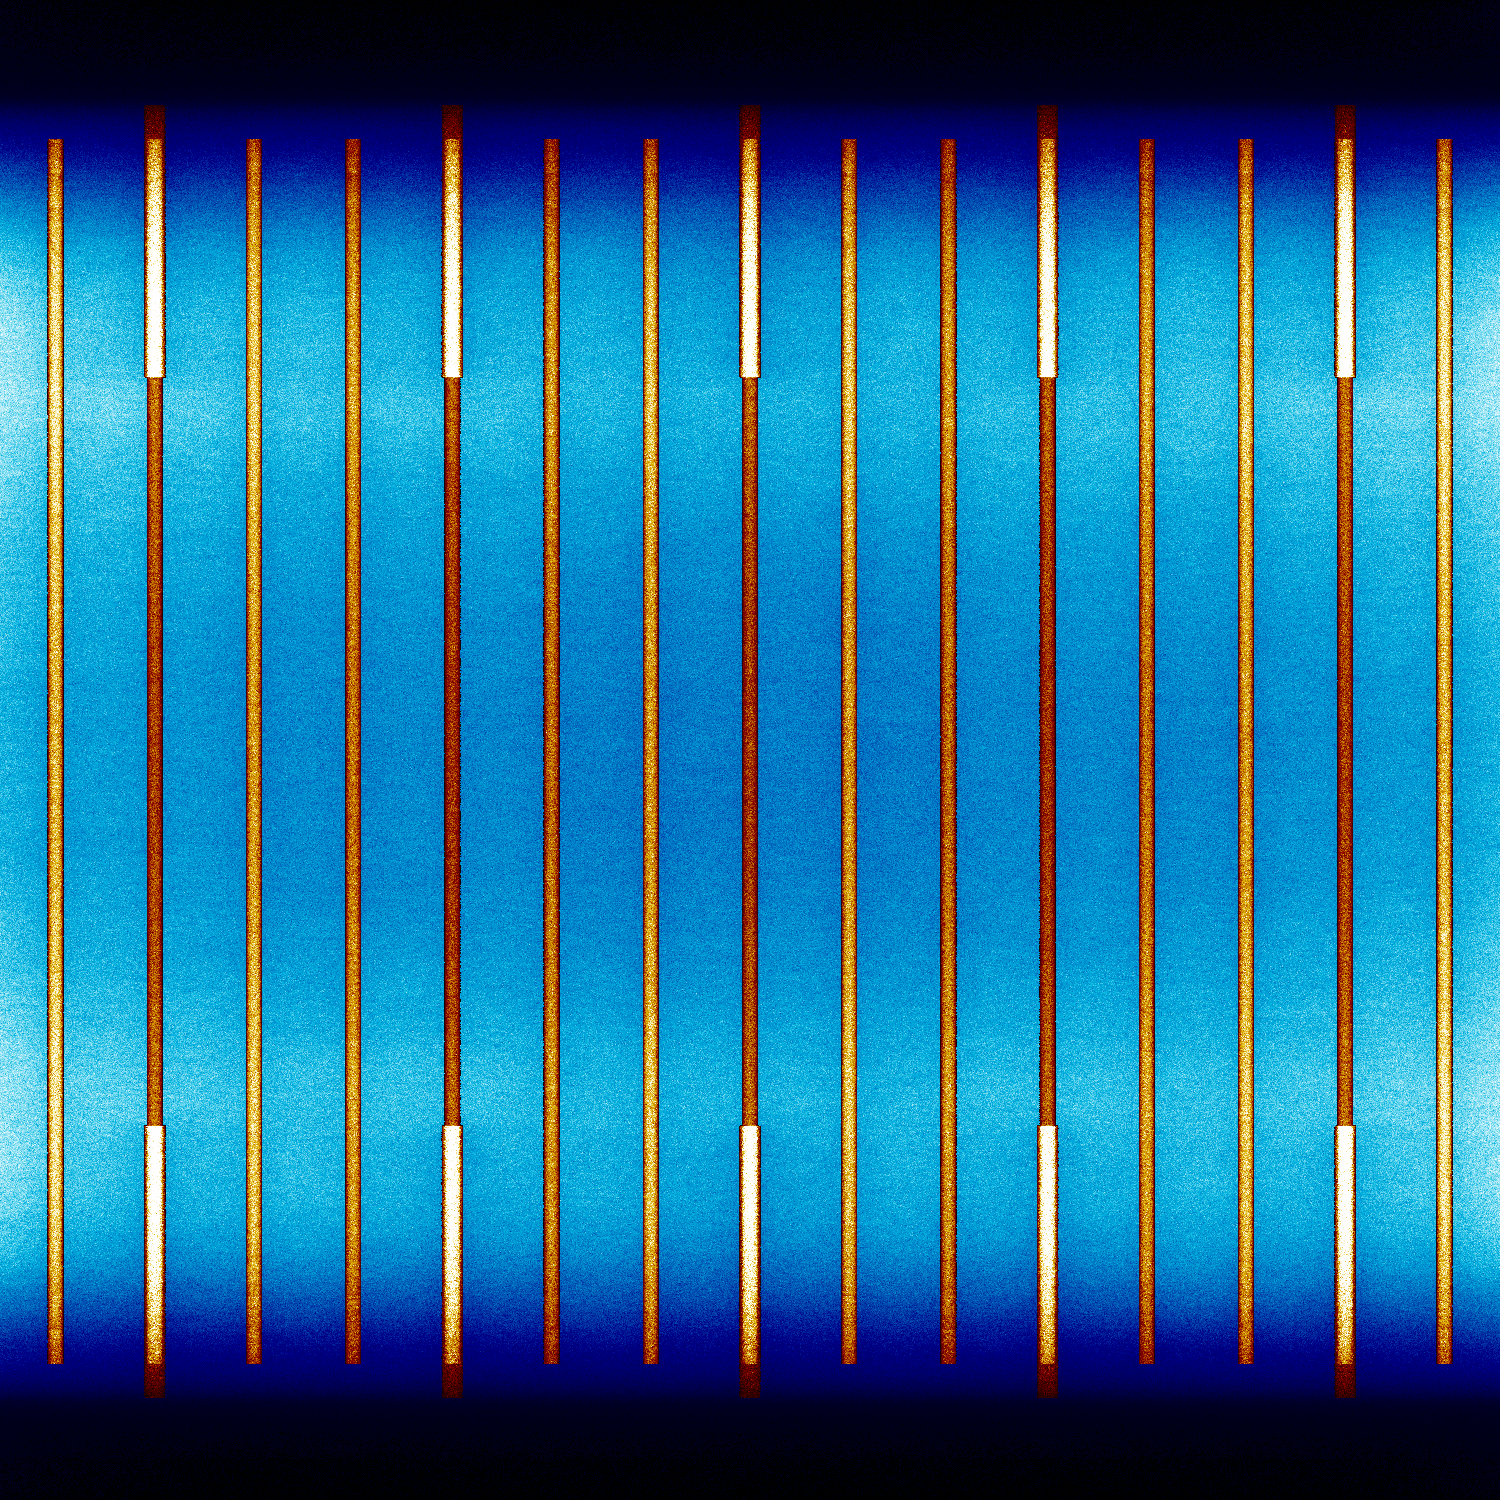
\includegraphics[width=\linewidth]{figs/powerdist-powerinverter.png}
        \caption{Power Inverter Device}
    \end{subfigure}

    \caption{Power distribution profiles under each mitigation strategy.}
\end{figure}

\usepackage{makecell} % in preamble

\begin{table}[H]
    \centering
    \renewcommand{\arraystretch}{1.8}
    \begin{tabular}{>{\bfseries\raggedright\arraybackslash}m{3.8cm} 
                    >{\centering\arraybackslash}m{1.2cm} 
                    >{\centering\arraybackslash}m{1.8cm} 
                    >{\centering\arraybackslash}m{1.5cm} 
                    >{\centering\arraybackslash}m{1.8cm} 
                    >{\centering\arraybackslash}m{1.5cm}}
    \toprule
    \textbf{Criteria} & \textbf{Weight} & \textbf{Do Nothing} & \textbf{Be Caps} & \textbf{Fresh Fuel} & \textbf{Power Inv.} \\
    \midrule
    Critical Cycle Length        & 0.4 & 1 & 1 & 4 & 3 \\
    Reliance on Spent Fuel       & 0.3 & 4 & 3 & 1 & 2 \\
    Utilization of lesser-depleted regions & 0.3 & 2 & 3 & 1 & 4 \\
    \midrule
    \textbf{Total} & \textbf{1.0} & \textbf{2.2} & \textbf{2.2} & \textbf{2.2} & \textbf{3.0} \\
    \bottomrule
    \end{tabular}
    \caption{Weighted decision matrix for mitigation strategies.}
\end{table}

Based upon the results of the 4 designs, it is justified to continue iterating upon the power inverter design. Because each simulation requires \>24 hours of wall time, a simplified model of the assembly was made using periodic boundary conditions -- as shown in Figure \ref{}. Although there are large discrepancies between the simplified model and higher-fidelity results, the simplified model completes the burnup simulation in \< 1 hour and provides general insight allowing for a large parametric sweep.

\begin{figure}[H]
    \centering
    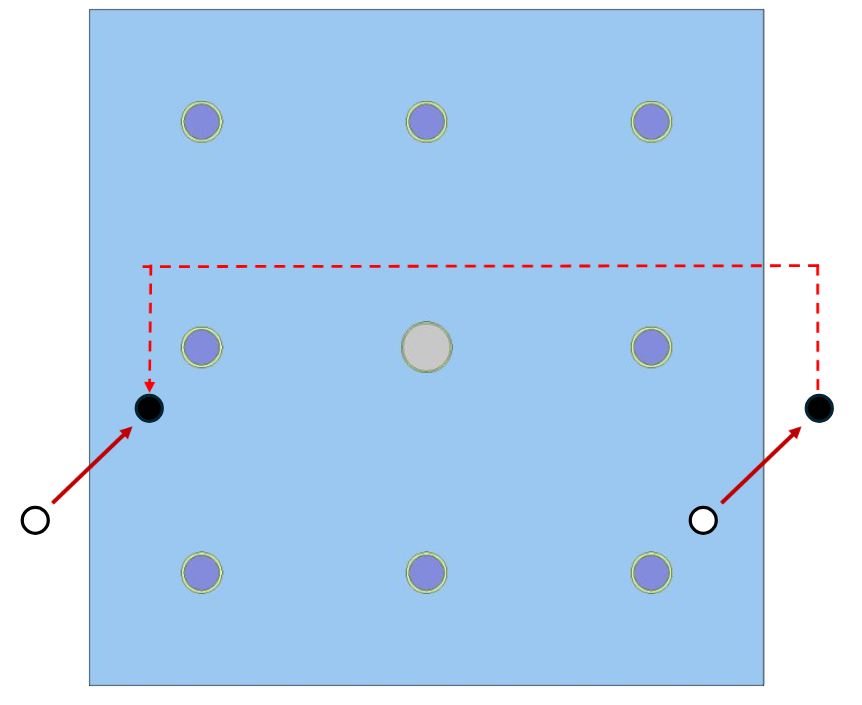
\includegraphics[width=0.5\linewidth]{figs/simplified-lbr.png}
    \caption{Enter Caption}
    \label{fig:placeholder}
\end{figure}

The parametric sweep was conducted for the length and enrichment of the fuel regions of the Power Inverter. Results for the CV and critical cycle length are shown in Figures \ref{} and \ref{} respectively.

\begin{figure}[H]
    \centering
    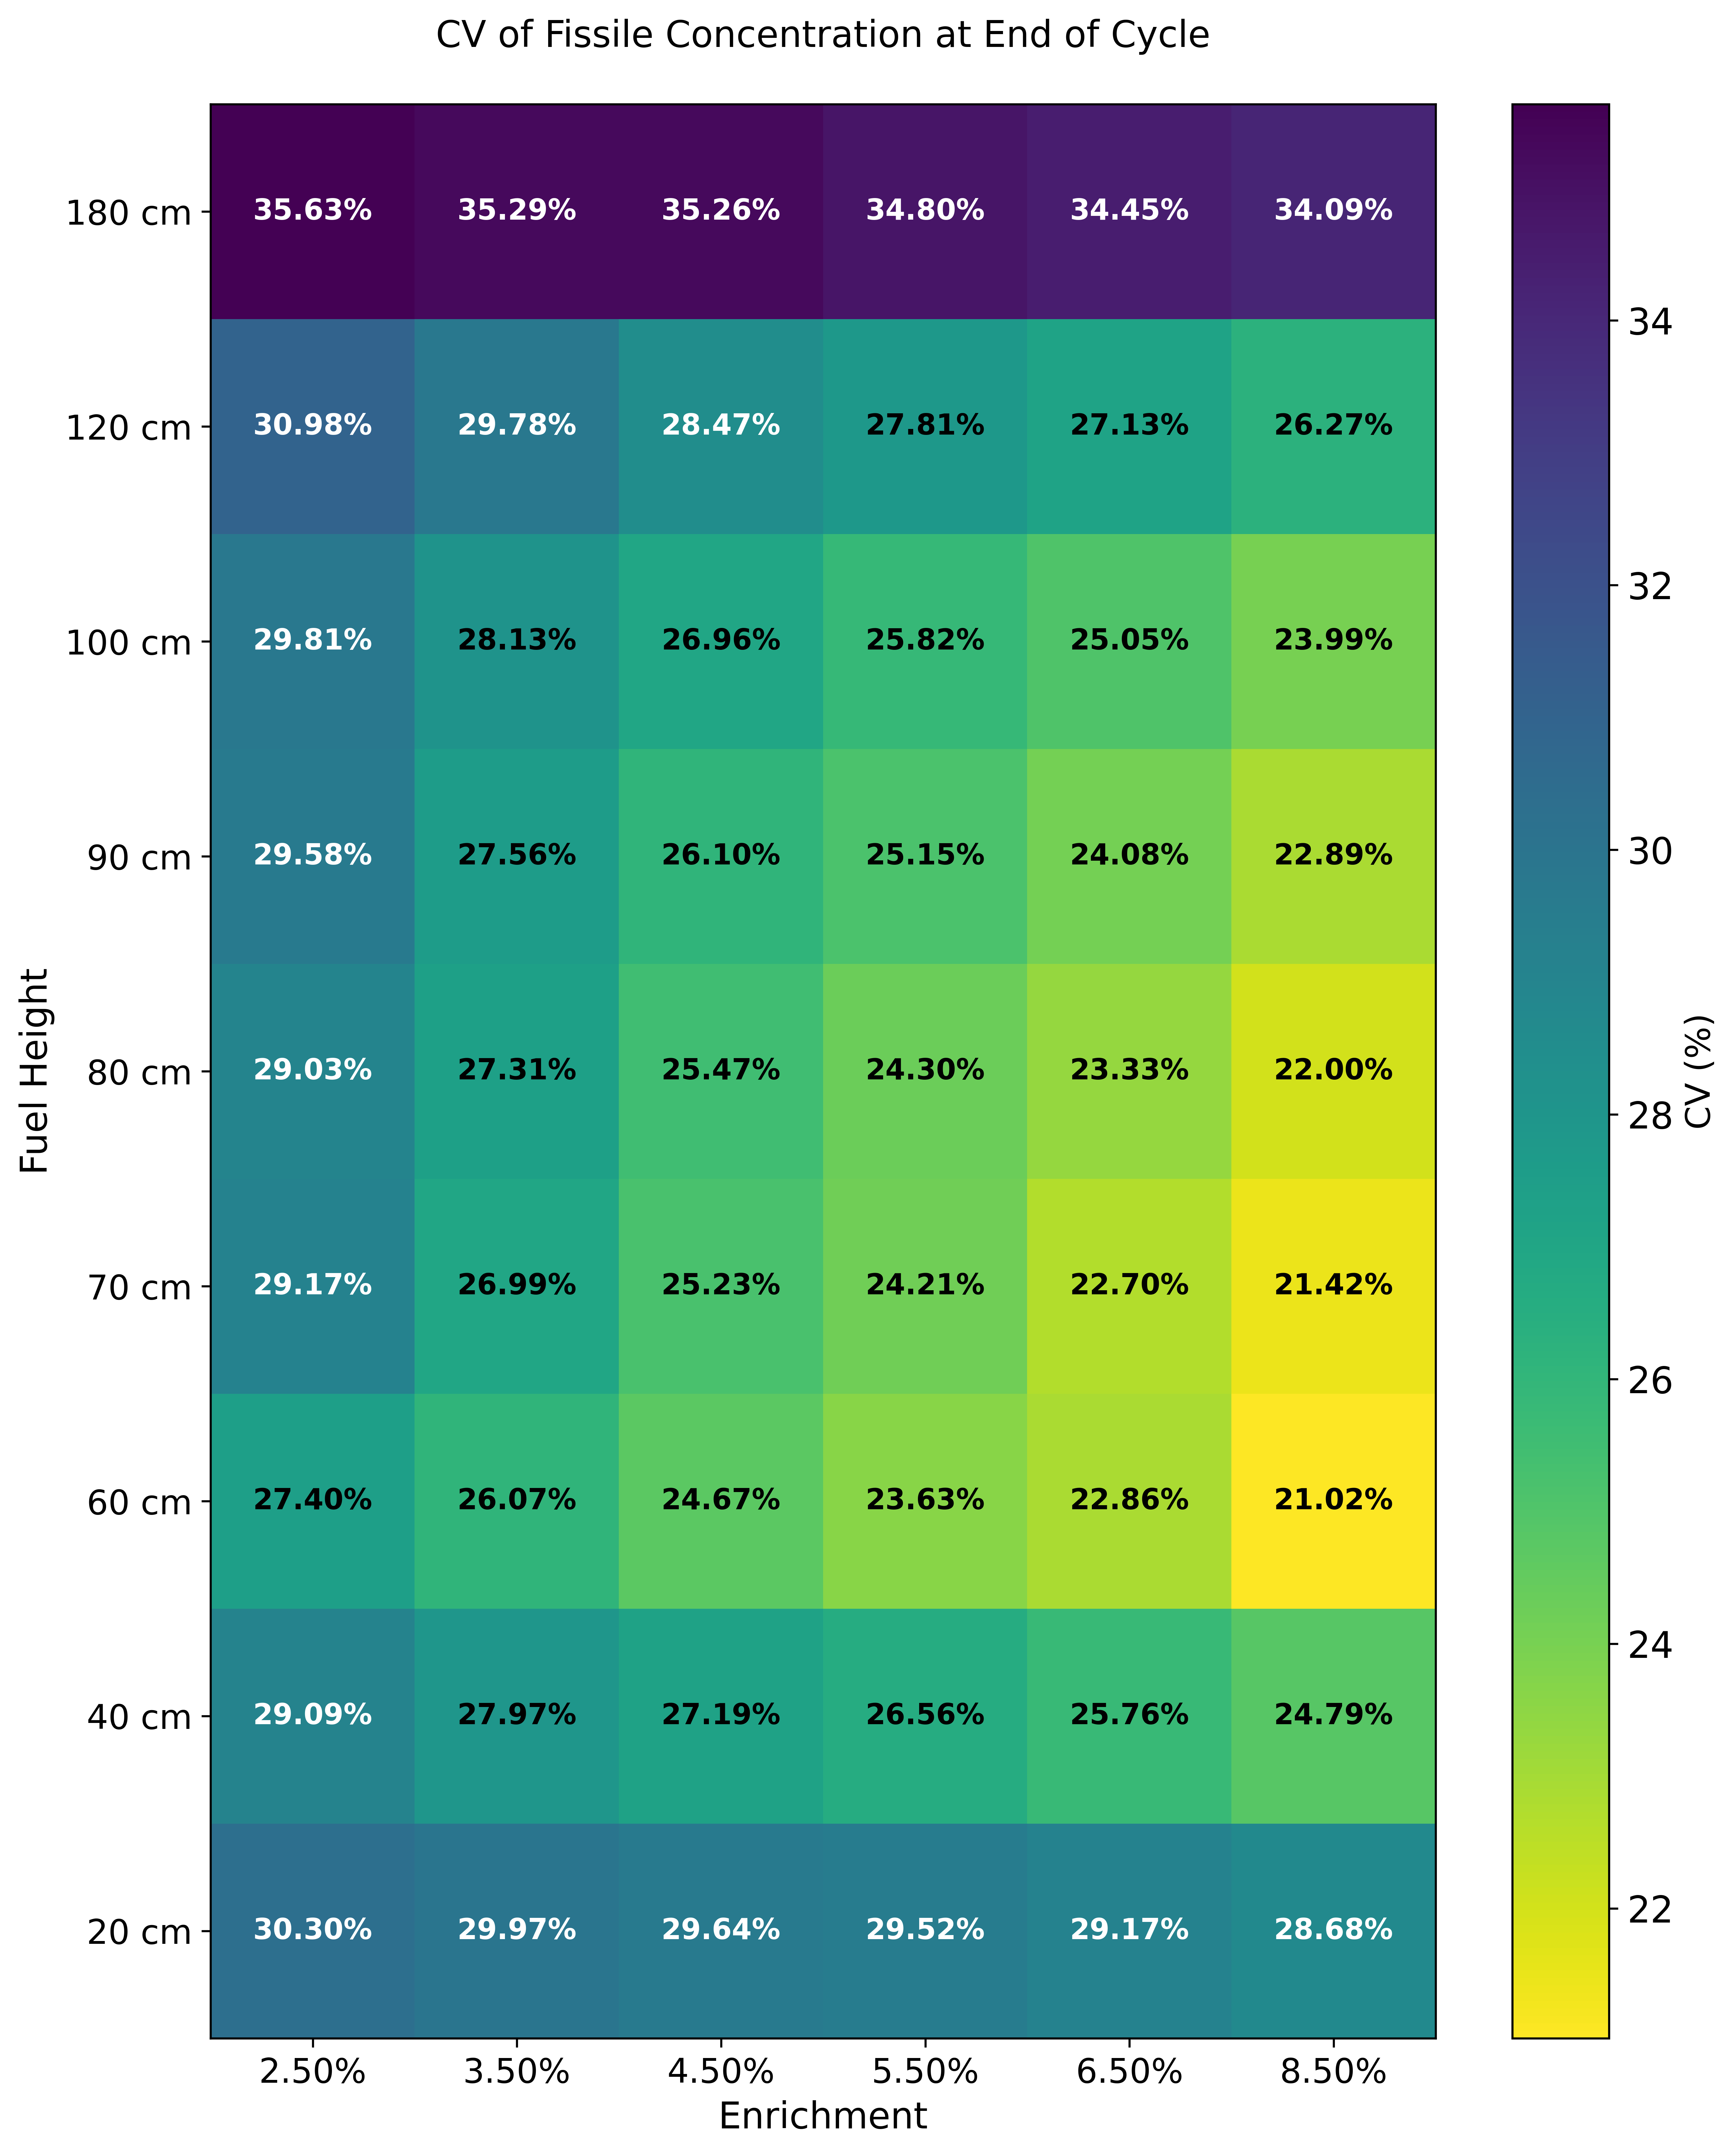
\includegraphics[width=0.8\linewidth]{figs/power-inverter-sweep-cv.png}
    \caption{Coefficient of variance results from power inverter parametric sweep. The length of fuel regions varied in height and enrichment. The study reveals that optimal length is between 60 and 80 cm}
    \label{fig:placeholder}
\end{figure}

\begin{figure}[H]
    \centering
    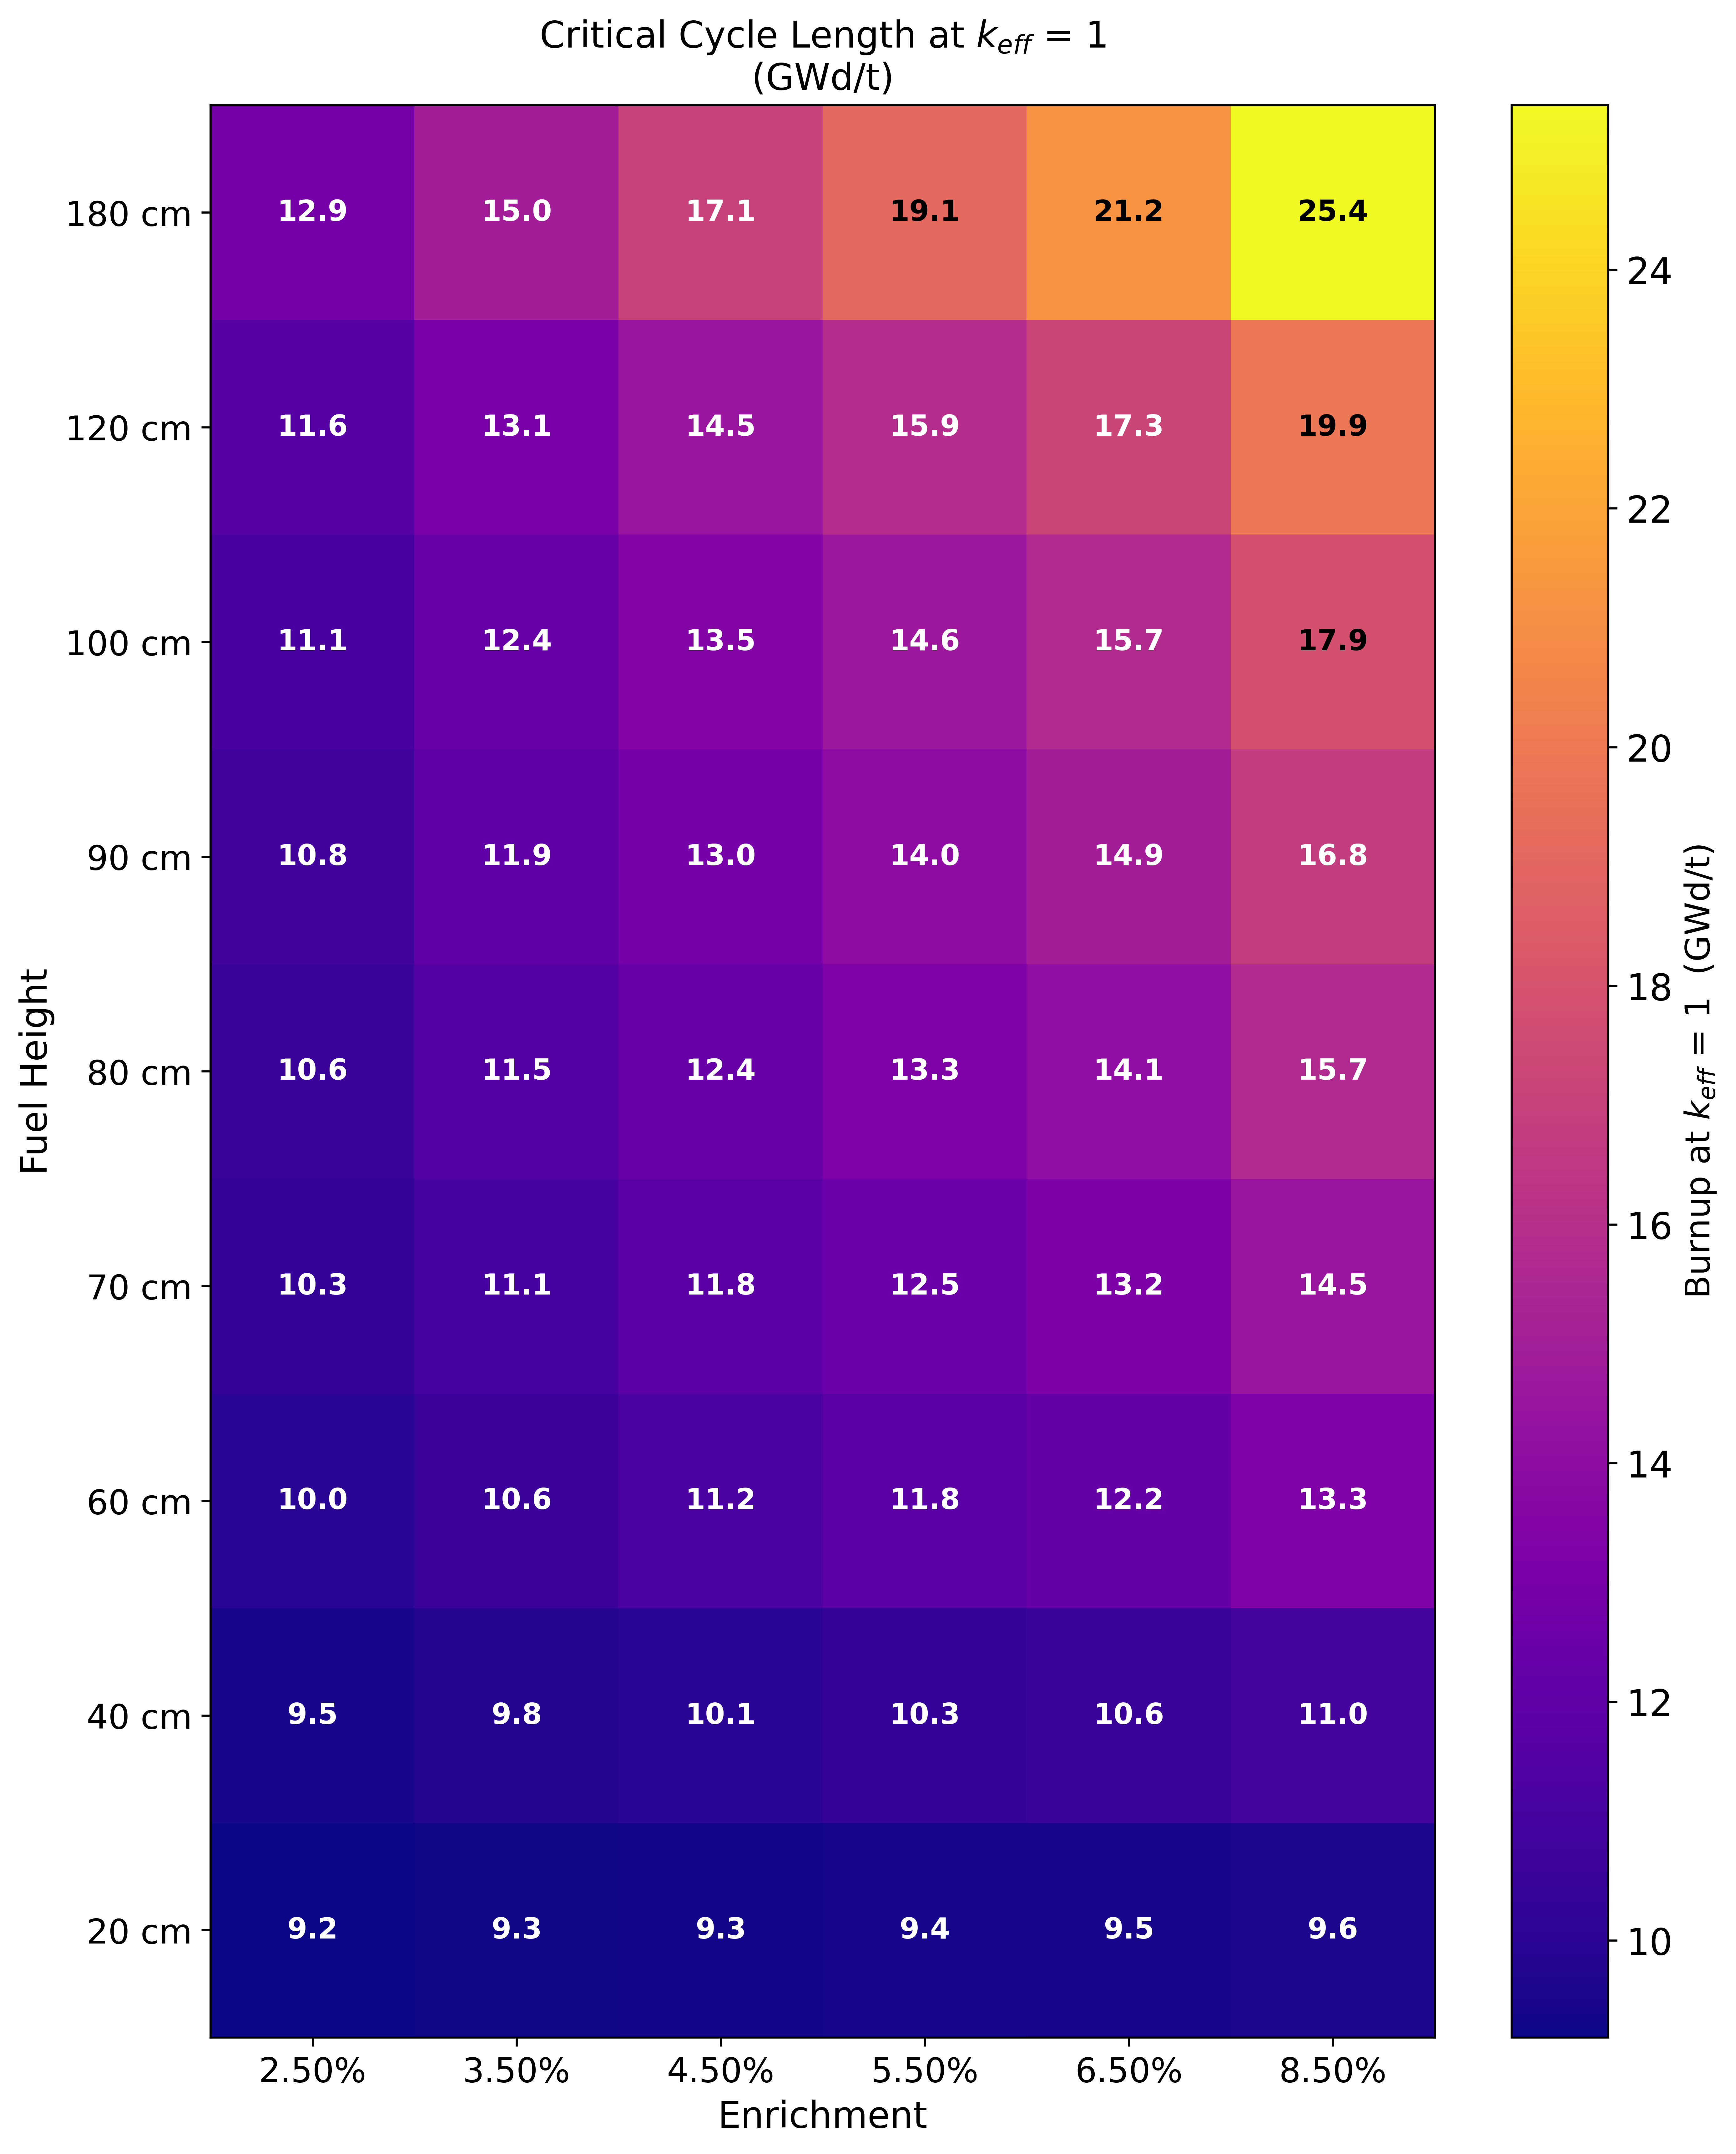
\includegraphics[width=0.8\linewidth]{figs/power-inverter-sweep-length.png}
    \caption{Enter Caption}
    \label{fig:placeholder}
\end{figure}

\clearpage

% ============================================================
% THERMAL HYDRAULICS
% ============================================================
\section{Thermal-Hydraulics and CFD Analysis (S. Yeatts)}
\label{sec:thermal-hydraulics}
The thermal--hydraulic analysis for the Last Breath Reactor (LBR) couples a high-fidelity CFD model of a representative coolant subchannel with an analytical radial conduction model for the fuel pin. The objective is to (i) quantify cladding and fuel temperatures at the design power density of 30~W/g, (ii) assess thermal margin relative to boiling crisis and material temperature limits, and (iii) establish a computationally inexpensive analytical surrogate that can be used to iterate over power density and operating conditions once validated against CFD. This section complements the neutronics and design-iteration sections by quantifying the thermal penalty associated with the 6~cm pitch selected for breeding performance and cycle length.

The authoritative thermal--hydraulic reference case is CFD case V5. This case corresponds to the average coolant channel in the 6~cm D$_2$O lattice at 10~MPa and 30~W/g, with the ANSYS Fluent energy equation enabled and thermophysical properties selected to represent irradiated spent fuel behavior rather than fresh-fuel PWR operation. The resulting area-averaged wall heat flux and heat transfer coefficient are consistent with the values adopted in the analytical conduction model, namely
\[
\bar{q}'' \approx 6.39\times 10^5\ \text{W/m}^2,
\qquad
\bar{h} \approx 757\ \text{W/m}^2\text{K}.
\]
These values are used throughout this section unless otherwise noted.

% ============================================================
\subsection{CFD Model Setup and Numerical Methodology}
\label{sec:cfd-setup}
% ============================================================

\subsubsection{Geometry and Progression of CFD Models}

A sequence of CFD models was developed to balance physical fidelity against computational cost. Case V3 is the final 4-pin subchannel model, in which four rods and the surrounding heavy-water coolant are modeled explicitly with symmetry applied at the outer boundaries. Cases V4 and V5 exploit single-pin symmetry to reduce computational expense while preserving the thermal and hydraulic environment of the repeated lattice. The purpose of the V3 $\rightarrow$ V4 transition was therefore to validate the use of geometric symmetry as a surrogate for the more expensive 4-pin calculation, while the V4 $\rightarrow$ V5 transition isolated the effect of introducing an explicit cladding region.

In V4, the pin was treated as a homogeneous solid with fuel properties only. In V5, the single-pin geometry was retained, but the solid domain was split into fuel and cladding regions, allowing cladding temperatures to be predicted more realistically. This distinction is important because the parameters of interest in the present study include cladding surface temperature and the radial distribution of temperature through the pin, both of which depend on whether the cladding is modeled explicitly.

The modeled pin geometry is based on the dimensions used throughout the project: a cladding outer radius of 5.46~mm, a fuel radius of 4.79~mm, and an active heated length of 3.60172~m. Although an analytical gas-gap model was later developed for comparison to fresh-fuel behavior, the CFD model does \emph{not} include an explicit gas gap. This is intentional. In spent fuel, pellet swelling, fission-product-induced relocation, cladding creep-down, and long-term thermo-mechanical contact can reduce or effectively eliminate the distinct helium gap that is present in fresh fuel. Accordingly, the spent-fuel CFD model represents the more realistic limiting configuration for this reactor concept, in which a distinct low-conductivity gas layer is no longer present between the pellet and cladding.

\subsubsection{Boundary Conditions, Fluid Model, and Solver Setup}

All CFD cases were performed in ANSYS Fluent using the pressure-based \cite{ANSYS_Fluent}, steady-state solver with the energy equation enabled. The SST \(k\)-\(\omega\) turbulence model was selected because it provides robust near-wall treatment in internal flows and is well suited to predicting wall shear and convective heat transfer in conjugate thermal problems. The coolant was modeled as heavy water at 10~MPa with representative thermophysical properties of \(\rho = 874\ \text{kg/m}^3\), \(c_p = 4670\ \text{J/kg-K}\), \(k = 0.53\ \text{W/m-K}\), and \(\mu = 1.14\times10^{-4}\ \text{kg/m-s}\).

For the V5 case, the fuel properties were taken as \(\rho = 10{,}196\ \text{kg/m}^3\), \(c_p = 330\ \text{J/kg-K}\), and \(k = 2.5\ \text{W/m-K}\), while the cladding properties were \(\rho = 6500\ \text{kg/m}^3\), \(c_p = 300\ \text{J/kg-K}\), and \(k = 9.2\ \text{W/m-K}\). These values intentionally represent degraded spent-fuel thermal conductivities rather than fresh-fuel PWR values. Their use is conservative in the sense that they increase radial conduction resistance within the solid, thereby increasing predicted temperatures for a given heat generation rate.

The fuel heat source in case V5 was prescribed as a volumetric energy generation of 305.88~MW/m\(^3\), corresponding to the nominal power density of 30~W/g for UO\(_2\) at the specified density. A mass-flow inlet was applied at 533.15~K, and the mass flow rate was chosen such that the average channel outlet temperature was 582.15~K, consistent with the scoping thermal--hydraulic calculation. Symmetry boundaries were applied on the lateral faces, and the outlet was prescribed as a pressure outlet at 0~Pa gauge relative to the 10~MPa operating pressure.

\subsubsection{Mesh Strategy and Near-Wall Resolution}

The final V5 mesh was generated using hexcore meshing with local refinement around the cladding and near-wall coolant region. Local sizing around the cladding used a target size on the order of the cladding thickness, together with boundary-layer inflation to resolve near-wall gradients. The resulting mesh contained approximately 17.8~million cells, 38.3~million faces, and 4.6~million nodes. The overwhelming computational cost arose from the need to simultaneously resolve the full axial length of 3.6~m and the thin solid layers at the rod surface, particularly the 0.67~mm cladding thickness.

\begin{figure}[H]
    \centering
    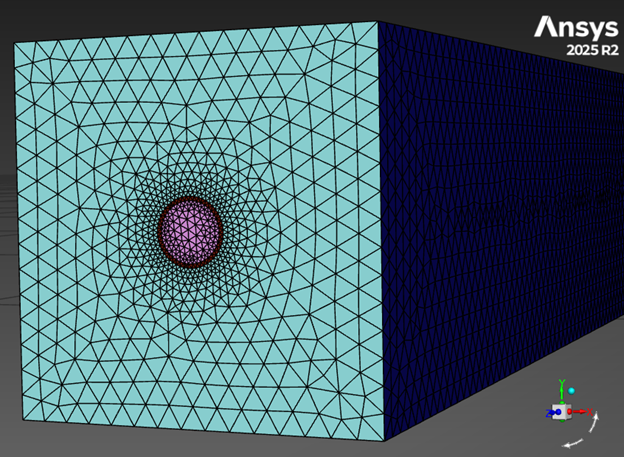
\includegraphics[width=0.5\linewidth]{figs/Mesh_SideProfile.png}
    \caption{Overall CFD mesh of the V5 single-pin conjugate heat transfer model, showing the full computational domain, symmetry boundaries, and the relative scale of the coolant, fuel, and cladding regions.}
    \label{fig:placeholder}
\end{figure}

\begin{figure}[H]
    \centering
    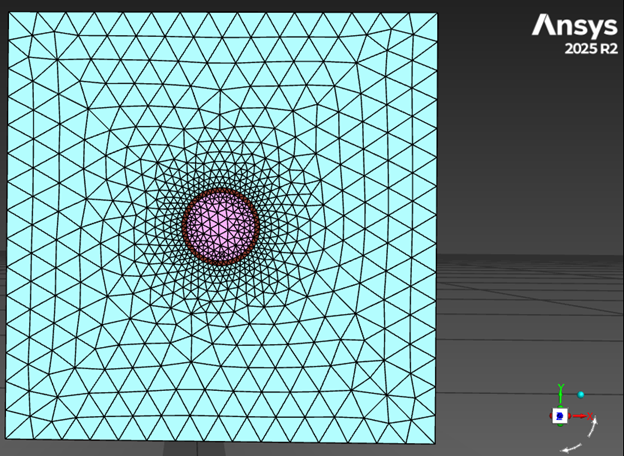
\includegraphics[width=0.48\linewidth]{figs/Mesh_Inlet.png}
    \hfill
    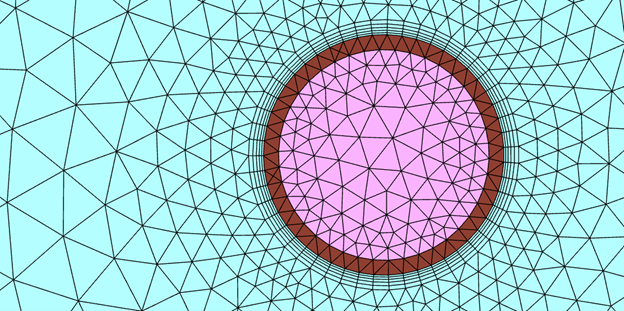
\includegraphics[width=0.48\linewidth]{figs/Mesh_FaceZoom.png}
    \caption{Detailed mesh views. Left: inlet mesh showing variable mesh sizing. Right: magnified inlet cross-section through the cladding and near-wall coolant region showing the mesh resolution used to capture thermal and velocity gradients at the wall via inflation layers and local sizing.}
    \label{fig:mesh_detail}
\end{figure}

A formal Grid Convergence Index (GCI) study was not practical for the final conjugate mesh. The dynamic length scale between the full subchannel length and the thin cladding region is extremely large, and the limiting factor in mesh refinement was the number of cells required inside and around the cladding. Increasing wall-normal resolution sufficiently to perform multiple systematically refined meshes would have increased cell count far beyond the already expensive 17~million-cell baseline, preventing meaningful design iteration within the available time and compute budget. For that reason, the CFD model was instead validated by comparing quantities of interest against reduced-domain CFD models and against an analytical radial conduction solution, as discussed below.

Near-wall resolution was assessed using the non-dimensional wall coordinate \(y^+\). In the final V5 model, the area-weighted-average cladding surface value was on the order of \(y^+ \approx 1.5\), and remained below 3 across the surface. This is desirable for the SST \(k\)-\(\omega\) model because it places the first grid point inside the viscous sublayer, allowing the wall-adjacent velocity and temperature gradients to be directly resolved rather than reconstructed through empirical wall functions. In the context of Reynolds-averaged Navier--Stokes (RANS) models, \(y^+\) provides a measure of whether the near-wall mixing-length behavior is being modeled in an appropriate regime; low \(y^+\) values indicate that the wall treatment is suitable for accurate heat transfer prediction.

\begin{figure}[H]
    \centering
    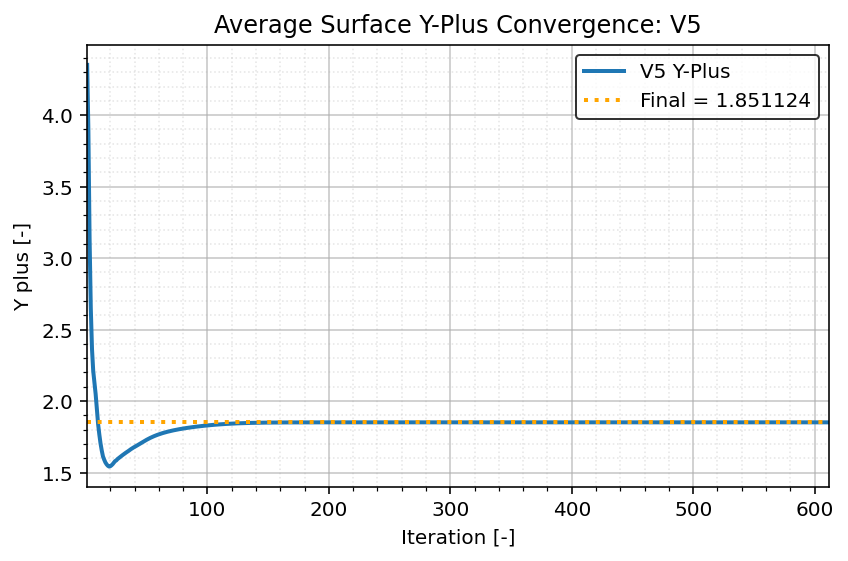
\includegraphics[width=0.6\linewidth]{figs/V5_YplusConv.png}
    \caption{Convergence of the area-weighted-average cladding-surface \(y^+\) for case V5, approaching a final value of about 1.85.}
    \label{fig:yplus_conv}
\end{figure}

\subsubsection{Why the CFD Model Omits an Explicit Gas Gap}

The omission of a gas gap in the CFD model is deliberate and physically motivated. In fresh PWR fuel, the helium-filled pellet--cladding gap is one of the dominant thermal resistances in the radial heat path, typically second only to the fuel itself. This gap produces a strong temperature drop between the fuel surface and the cladding inner wall. In spent fuel, however, irradiation-driven swelling, relocation, cracking, and cladding creep-down tend to reduce or close the original gap, producing direct or near-direct contact over substantial fractions of the interface. As a result, an explicit gas layer is not necessarily the best representation of the spent-fuel thermal state relevant to the LBR concept.

This has two competing effects on the radial temperature distribution. First, the degraded thermal conductivity of irradiated fuel and conservative cladding conductivity values increase solid-phase thermal resistance, tending to raise fuel centerline and cladding temperatures. Second, the absence of the gas gap removes what is normally one of the most influential thermal resistances in fresh-fuel PWR operation. This reduction in interfacial insulation tends to increase conductive coupling between the hot fuel and the cladding, which can raise cladding temperatures even while reducing the sharp temperature drop that would otherwise occur across the gap. The temperature field in spent fuel therefore differs qualitatively from that of fresh fuel: the profile becomes more tightly coupled between fuel and cladding, with larger fractions of the total temperature drop occurring within the degraded fuel itself.

A thin exterior coating on the cladding was also considered qualitatively. However, the materials technical expert on the project indicated that the coating thermal conductivity is sufficiently high that its effect on the temperatures of interest is negligible compared to the dominant resistances in the fuel, cladding, coolant-side convection, and, where applicable, the gas gap. The coating was therefore omitted from the CFD and analytical models without loss of fidelity for the present scoping-level objectives.

% ============================================================
\subsection{Analytical Radial Conduction Model and Comparison to CFD}
\label{sec:analytic-vs-cfd}
% ============================================================

\subsubsection{Closed-Form Radial Conduction Model}

To enable rapid iteration over heat generation rates and material properties, an analytical radial conduction model was developed for concentric cylindrical regions under steady, axisymmetric conditions. The base form includes a fuel region with uniform volumetric heat generation and a cladding region with no internal heat generation. The governing equation is
\[
\frac{1}{r}\frac{d}{dr}\left(k\,r\,\frac{dT}{dr}\right) + \dot{q} = 0,
\]
with the usual parabolic solution in the fuel and logarithmic solution in the cladding.

\begin{figure}[H]
    \centering
    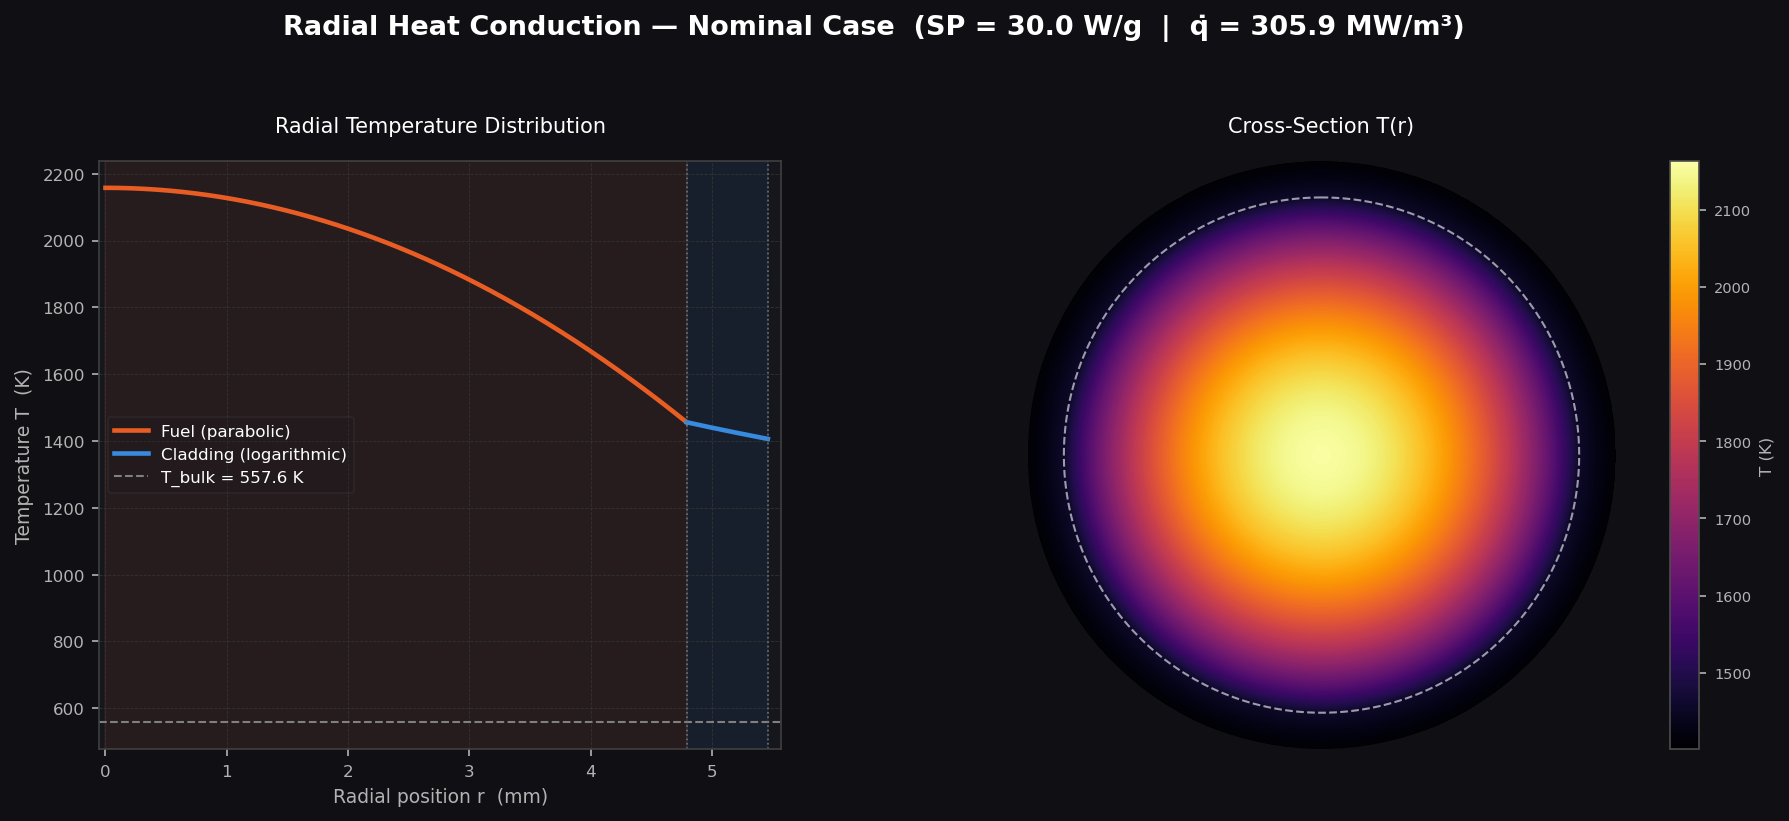
\includegraphics[width=0.9\linewidth]{figs/nominal_case.png}
    \caption{Analytical radial heat conduction for the nominal case at 30~W/g. Left: radial temperature distribution in fuel and cladding with bulk coolant temperature indicated. Right: 2-D cross-section temperature map showing the parabolic fuel and logarithmic cladding profile.}
    \label{fig:nominal_analytic}
\end{figure}

A more detailed version of the model was then extended to include an explicit gas gap and higher fresh-fuel thermal conductivities for comparison to normal PWR behavior. This analytical model does not represent the CFD case directly, since the CFD omits the gap, but it is useful for understanding the relative roles of degraded thermal conductivity and gas-gap resistance. In particular, it shows that adding a gas gap introduces a large additional temperature drop between fuel and cladding, while increasing fuel and cladding conductivities reduces the temperature rise required to conduct a given heat load. The spent-fuel case considered here is therefore characterized by two simultaneous changes relative to fresh fuel: increased conduction resistance in the fuel and cladding due to degraded conductivity, and removal of a major resistance due to gap closure. These effects partially offset one another in terms of centerline temperature, but they tend to increase cladding temperature because the cladding is more directly thermally coupled to the hotter fuel.

\subsubsection{Boundary Conditions and CFD-Calibrated Comparison}

Two outer boundary-condition strategies were evaluated in the analytical model. In the first, the cladding outer surface was assigned a uniform heat flux equal to the CFD-derived average value,
\[
q'' \approx 6.3904866\times10^5\ \text{W/m}^2,
\]
and the surface temperature was then obtained through the convective closure
\[
q'' = h(T_\text{surf} - T_\text{bulk}),
\]
using the CFD-derived average \(h \approx 757.46\ \text{W/m}^2\text{K}\) and
\[
T_\text{bulk} = \frac{T_\text{in} + T_\text{out}}{2}
= \frac{533.15 + 582.15}{2}
= 557.65\ \text{K}.
\]

In the second strategy, the CFD surface-averaged cladding temperature itself was imposed directly as a Dirichlet boundary condition in the analytical model. This was done because the conjugate CFD solution intrinsically captures local variations in convection coefficient, circumferential heat flux, and coolant temperature, whereas a single average heat flux and average heat transfer coefficient cannot fully represent those three-dimensional effects.

\begin{figure}[H]
    \centering
    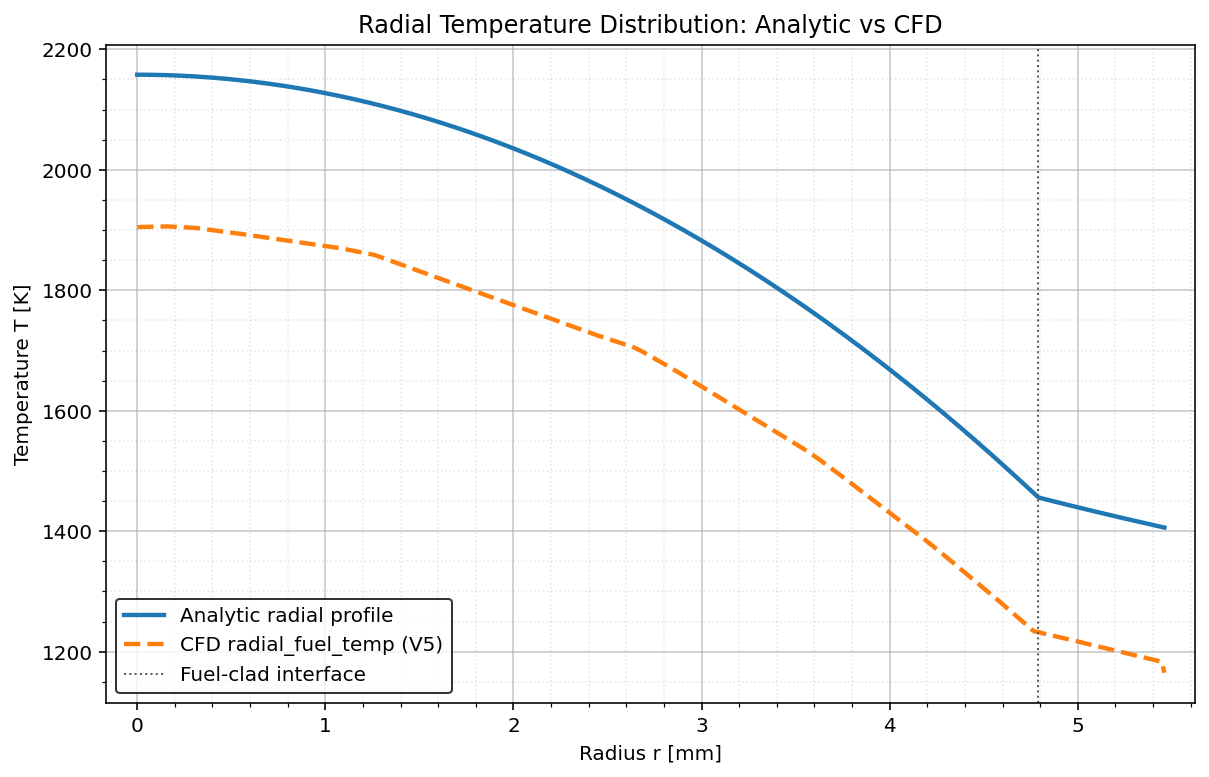
\includegraphics[width=0.75\linewidth]{figs/V5_CompareRadialTemp_Flux.png}
    \caption{Comparison between analytical and CFD radial temperature distributions for case V5 using a flux-based outer boundary condition. The flux-based analytical model overpredicts temperatures relative to CFD because it cannot capture the spatially varying convection present in the full conjugate solution.}
    \label{fig:radial_compare_flux}
\end{figure}

\begin{figure}[H]
    \centering
    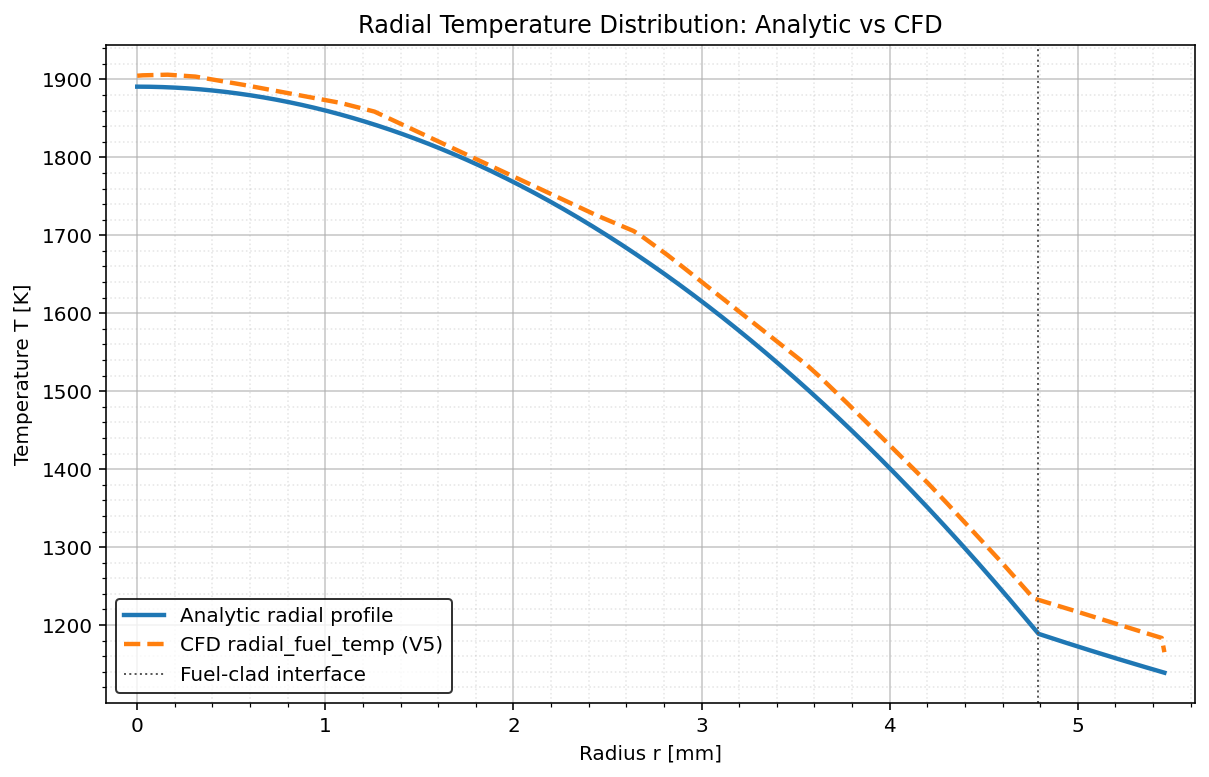
\includegraphics[width=0.75\linewidth]{figs/V5CompareRadialTemp_Temp.png}
    \caption{Comparison between analytical and CFD radial temperature distributions for case V5 when the outer boundary is set by the CFD surface-averaged cladding temperature. Using the CFD surface temperature as a Dirichlet boundary condition yields much closer agreement with the CFD radial profile.}
    \label{fig:radial_compare_temp}
\end{figure}

The comparison shows that the prescribed heat-flux boundary condition over-predicts the radial temperature distribution relative to CFD. This result is consistent with the large implied convective temperature rise,
\[
\Delta T_\text{conv} = \frac{q''}{h}
\approx \frac{6.39\times10^5}{757}
\approx 844\ \text{K},
\]
which is unrealistically severe when interpreted as a uniformly applied condition over the entire rod perimeter. In the CFD model, by contrast, the coupled solution with the energy equation enabled distributes temperature and heat transfer more realistically in space, producing lower and more credible wall temperatures for the average channel. Consequently, using the CFD surface-averaged temperature as the outer boundary condition in the analytical model provides substantially better agreement with the CFD radial temperature profile than using the average surface heat flux.

This observation is important for design iteration. The flux-based analytical model is conservative and therefore useful for screening and bounding calculations. However, because it overestimates the temperature profile relative to the CFD solution, it is not the best tool for iterating over power density once a CFD reference state is available. The temperature-prescribed analytical model is more appropriate for interpolation and sensitivity studies around the validated CFD operating point.

\subsubsection{Radial and Axial Temperature Behavior in V5}

The V5 CFD solution also provides detailed information about axial trends. At the fuel centerline, the temperature rises from roughly 1500~K near the inlet to about 1900~K near the outlet, with a global mean of approximately 1857~K.

\begin{figure}[H]
    \centering
    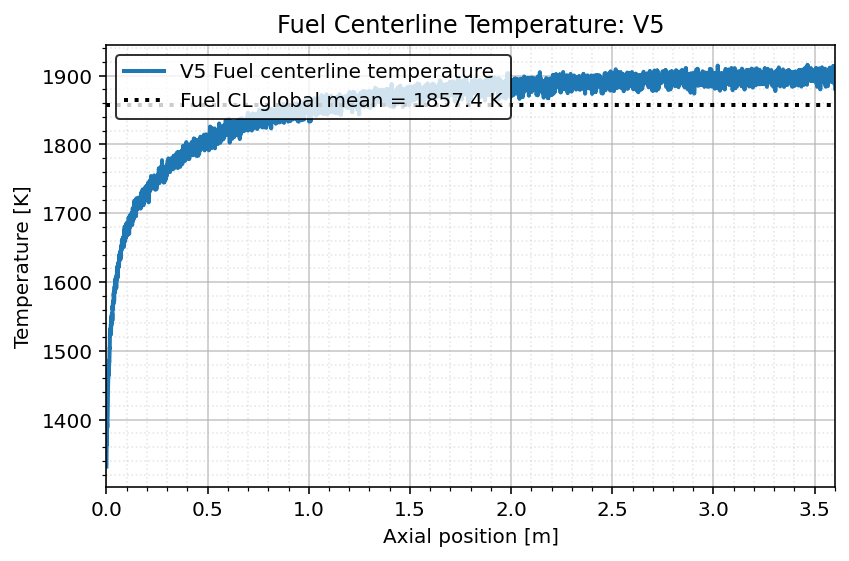
\includegraphics[width=0.6\linewidth]{figs/V5FuelCenterTemp.png}
    \caption{Fuel centerline temperature along the heated length for case V5, with the global mean indicated by the dashed line.}
    \label{fig:v5_centerline_temp}
\end{figure}

A radial cut through the fuel at a fixed axial location near the outlet shows a monotonic decrease from centerline temperature to the fuel--cladding interface, where the temperature is approximately 1400--1450~K depending on the exact axial position.

\begin{figure}[H]
    \centering
    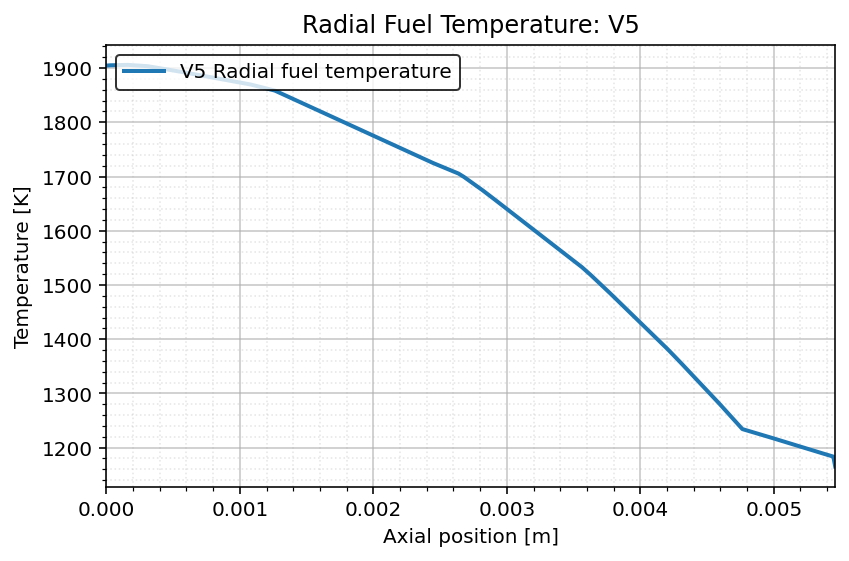
\includegraphics[width=0.6\linewidth]{figs/V5RadialFuelTemp.png}
    \caption{Radial fuel temperature near the outlet for case V5, extracted along a line from the fuel centerline to the fuel--cladding interface.}
    \label{fig:v5_radial_cut}
\end{figure}

\subsubsection{Effect of the 6~cm Pitch on Mass Flux and Heat Transfer}

The 6~cm pitch selected by the neutronics optimization is far larger than the rod pitches of conventional light-water reactor fuel bundles. This larger pitch increases coolant flow area per rod and therefore reduces the mass flux for a given total flow rate. In the scoping thermal--hydraulic calculation, the resulting average-channel mass flux is
\[
G = 102.6\ \text{kg/m}^2\text{s},
\]
for heavy water at 10~MPa. This is substantially lower than mass fluxes typical of commercial PWR rod bundles, which are often on the order of \(10^3\) to \(4\times10^3\ \text{kg/m}^2\text{s}\).

The reduced mass flux has a direct thermal consequence: it lowers the Reynolds number and therefore reduces the convective heat transfer coefficient. That is the dominant reason the CFD-reported average heat transfer coefficient for the LBR channel is only about \(757\ \text{W/m}^2\text{K}\), whereas typical PWR channels often exhibit values one order of magnitude higher. In other words, the same large pitch that improves neutronic breeding potential also degrades heat removal capability.

Using the hydraulic diameter associated with the 6~cm pitch channel and the V5 fluid properties, the Reynolds number remains in the turbulent regime, but at the low end relative to commercial LWR practice. This is sufficient to justify turbulence modeling, but it also explains why the LBR coolant channel behaves less like a tightly packed high-flux PWR bundle and more like a relatively open moderated passage with modest wall heat transfer.

\begin{figure}[H]
    \centering
    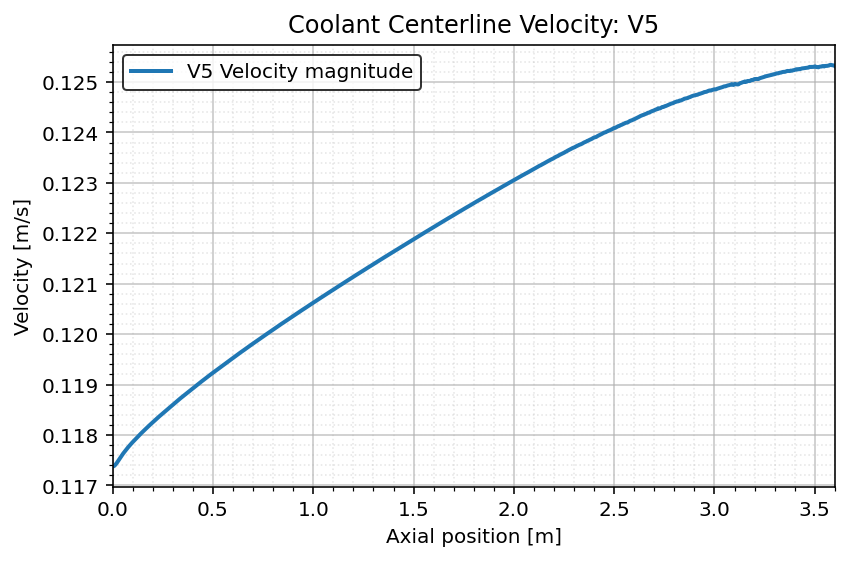
\includegraphics[width=0.6\linewidth]{figs/V5Velocity.png}
    \caption{Coolant centerline velocity along the heated length for case V5, illustrating the low but still turbulent mass flux associated with the 6~cm pitch.}
    \label{fig:v5_velocity}
\end{figure}

\begin{figure}[H]
    \centering
    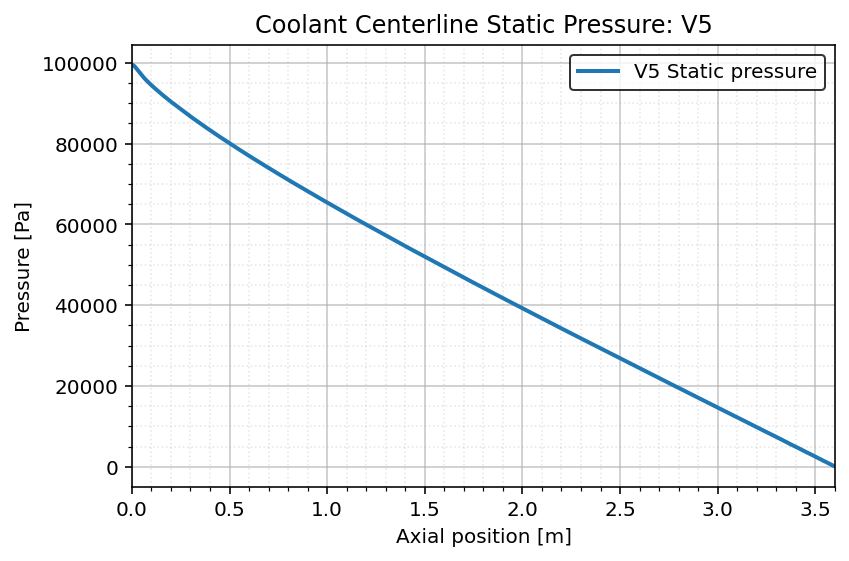
\includegraphics[width=0.6\linewidth]{figs/V5Pressure.png}
    \caption{Coolant centerline static pressure for case V5, showing the pressure drop along the heated length.}
    \label{fig:v5_pressure}
\end{figure}

\subsubsection{Surface Heat Flux and Heat Removal Capability}

For the 30~W/g average channel, the relevant surface heat flux is approximately
\[
\bar{q}'' \approx 639\ \text{kW/m}^2.
\]
This is not exceptionally large compared to commercial reactor practice; what makes it thermally challenging in the present design is the low coolant-side heat transfer coefficient caused by the low mass flux and large pitch. A moderate heat flux combined with a weak convective sink can still produce high cladding temperatures. This distinction is important: the temperature challenge in the LBR is driven less by unusually extreme heat flux and more by the fact that the pitch required for neutronic performance inherently weakens heat removal.

\begin{figure}[H]
    \centering
    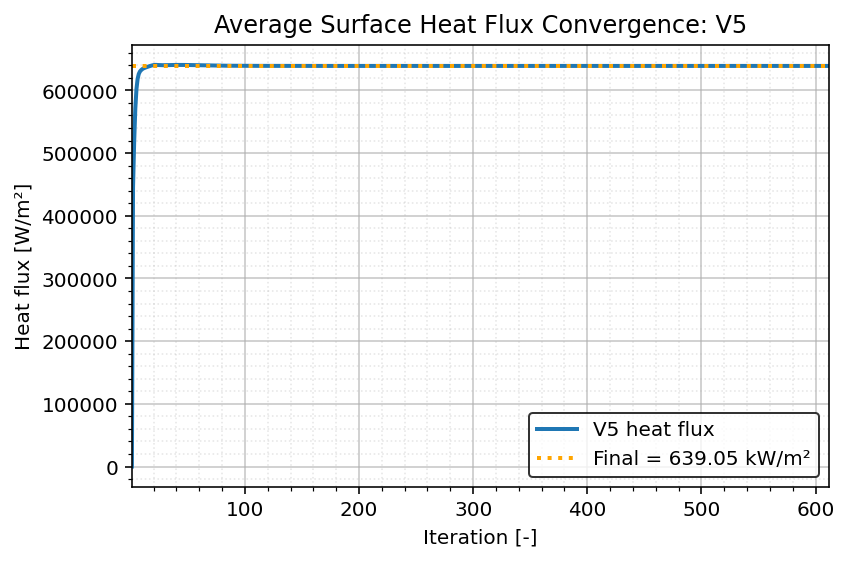
\includegraphics[width=0.6\linewidth]{figs/V5_FluxConv.png}
    \caption{Convergence history of the surface-averaged heat flux in case V5, approaching a final value of approximately 639~kW/m\(^2\).}
    \label{fig:v5_flux_conv}
\end{figure}

\begin{figure}[H]
    \centering
    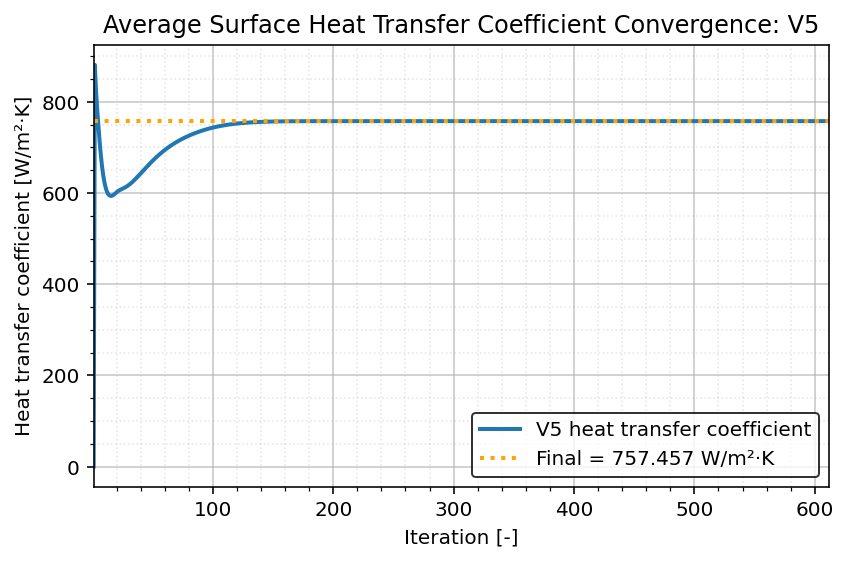
\includegraphics[width=0.6\linewidth]{figs/V5_hConv.png}
    \caption{Surface-averaged heat transfer coefficient convergence for case V5, with a final value near 757~W/m\(^2\)K.}
    \label{fig:v5_h_conv}
\end{figure}

% ============================================================
\subsection{DNBR and Thermal Margin}
\label{sec:dnbr}
% ============================================================

To assess margin to departure from nucleate boiling, DNBR was evaluated using the specified conditions of 10~MPa, heavy water coolant, 6~cm pitch, and a mass flux of \(102.6\ \text{kg/m}^2\text{s}\), with the power peaking factor applied to obtain a hot-channel estimate. The average-channel wall heat flux at 30~W/g is approximately \(639\ \text{kW/m}^2\). Applying the project-relevant power peaking factor of approximately 2.2 yields a peak heat flux of
\[
q''_\text{peak} \approx 2.2 \times 639\ \text{kW/m}^2
\approx 1.41\ \text{MW/m}^2.
\]

Because the power peaking factor is elevated by the introduction of spent fuel for burnup redistribution, the hot channel is the more relevant thermal-limiting case. In the neutronics-driven design iteration, the PPF increased from values near 1.7 in the more conventional baseline configurations to values above 2.2 in the spent-fuel power-shaping configurations. This improves fissile utilization and cycle behavior but directly increases the local thermal burden, since peak temperature and DNBR scale much more strongly with local power than with assembly-average power. The thermal analysis therefore links the neutronics benefit of spent-fuel insertion to a thermal penalty that must be carefully managed.

The final DNBR should be reported using the Groeneveld 2006 LUT value extracted at the operating pressure, mass flux, and quality corresponding to the V5 average-channel condition \cite{Groeneveld2007TheTable}. The governing definition is
\[
\text{DNBR} = \frac{q''_\text{CHF}}{q''_\text{local}},
\]
with \(q''_\text{local}\) taken as either the average-channel heat flux or the PPF-scaled hot-channel heat flux. Using a simple linear interpolation of the Groeneveld LUT, the resulting DNBR values are greater than 2.9 for both the average-channel and peak-channel conditions, which provides more than adequate thermal margin:
\[
q''_\text{CHF, Groeneveld} = \text{4.163}\ \text{MW/m}^2,
\]
\[
\text{DNBR}_\text{avg} = \frac{q''_\text{CHF, Groeneveld}}{0.639\ \text{MW/m}^2} = 6.5,
\qquad
\text{DNBR}_\text{peak} = \frac{q''_\text{CHF, Groeneveld}}{1.41\ \text{MW/m}^2} = 2.95.
\]

The full CHF scoping methodology, including governing equations, parameter table, sensitivity study, and comparison to typical reactor values, is documented in Section~\ref{sec:th-scoping}.

% ============================================================
\subsection{Comparison of 4-Pin and Single-Pin Models}
\label{sec:v3-v5-comparison}
% ============================================================

Because the final conjugate CFD mesh was computationally expensive, the single-pin symmetric models were validated against the final 4-pin model before being adopted for the rest of the thermal workflow. The V3 model represents the last 4-pin calculation, while V4 and V5 are both single-pin models. The V3 $\rightarrow$ V4 comparison isolates the effect of exploiting symmetry for computational savings, while the V4 $\rightarrow$ V5 comparison isolates the effect of explicitly modeling cladding.

\begin{figure}[H]
    \centering
    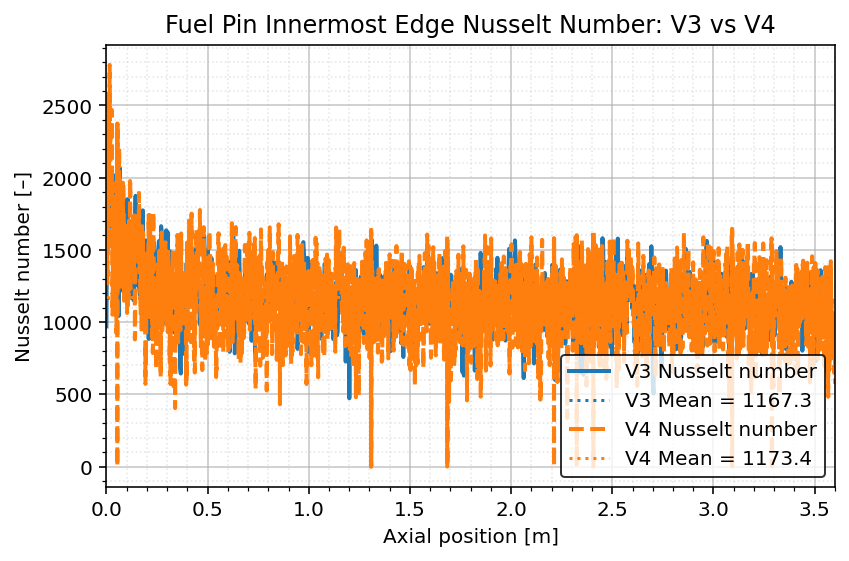
\includegraphics[width=0.75\linewidth]{figs/V3V4_Nu.png}
    \caption{Fuel pin innermost-edge Nusselt number for V3 versus V4. The mean Nusselt numbers agree within about 0.5\%, validating the use of single-pin symmetry for convective heat transfer prediction.}
    \label{fig:v3v4_nu}
\end{figure}

\begin{figure}[H]
    \centering
    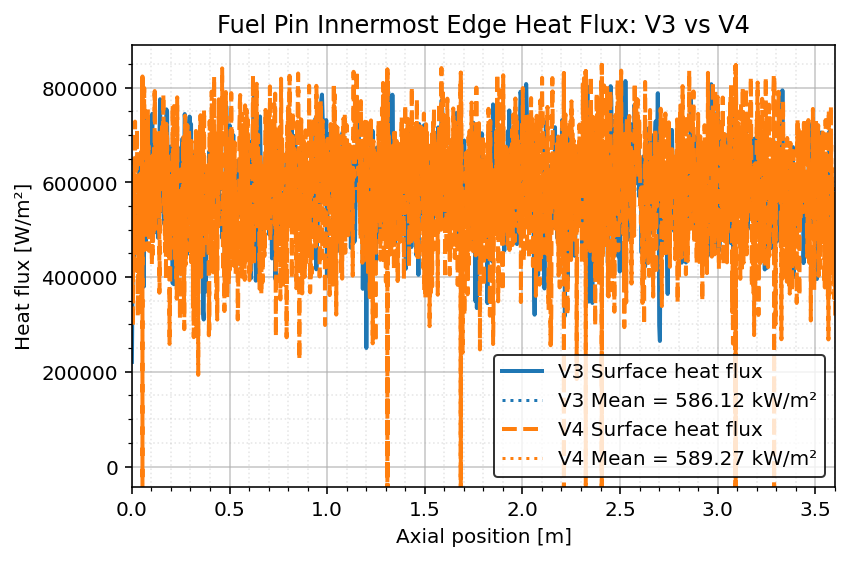
\includegraphics[width=0.75\linewidth]{figs/V3V4CladHeatFlux.png}
    \caption{Fuel pin innermost-edge surface heat flux for V3 versus V4. Mean heat fluxes differ by only a few kW/m\(^2\), indicating that the single-pin model reproduces the 4-pin heat-transfer behavior.}
    \label{fig:v3v4_q}
\end{figure}

\begin{figure}[H]
    \centering
    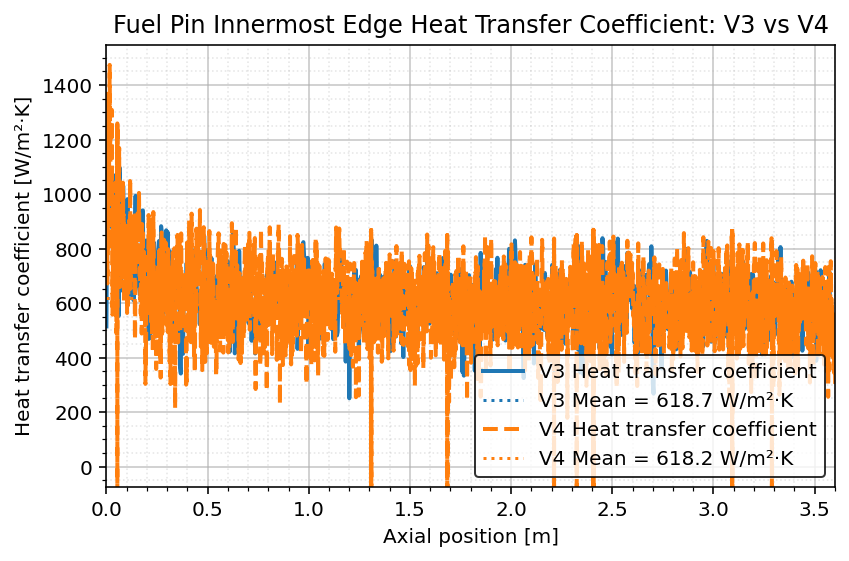
\includegraphics[width=0.75\linewidth]{figs/V3V4_h.png}
    \caption{Fuel pin innermost-edge heat transfer coefficient for V3 versus V4, again showing excellent agreement between the 4-pin and single-pin geometries.}
    \label{fig:v3v4_h}
\end{figure}

\begin{figure}[H]
    \centering
    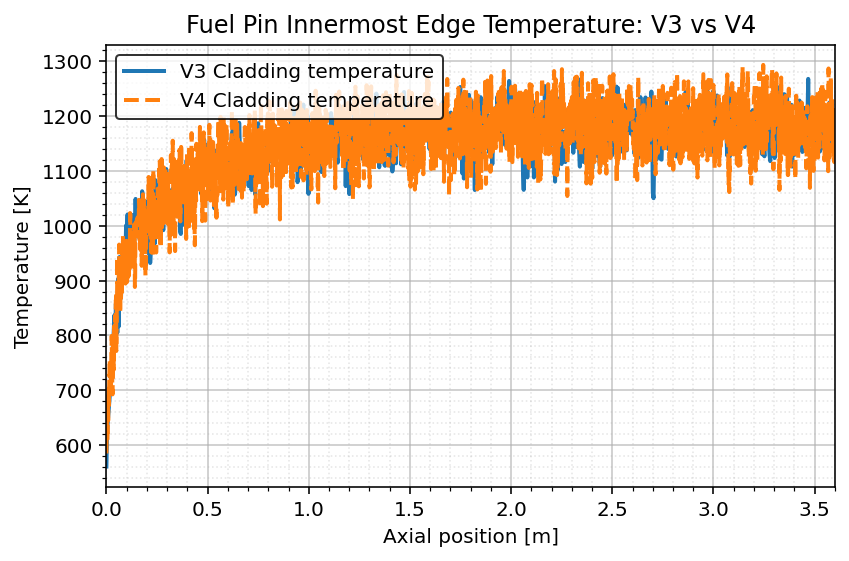
\includegraphics[width=0.75\linewidth]{figs/V3V4CladTemp.png}
    \caption{Cladding temperature at the innermost fuel pin edge for V3 versus V4, demonstrating that the single-pin model preserves the axial temperature distribution of the 4-pin reference.}
    \label{fig:v3v4_cladT}
\end{figure}

\begin{figure}[H]
    \centering
    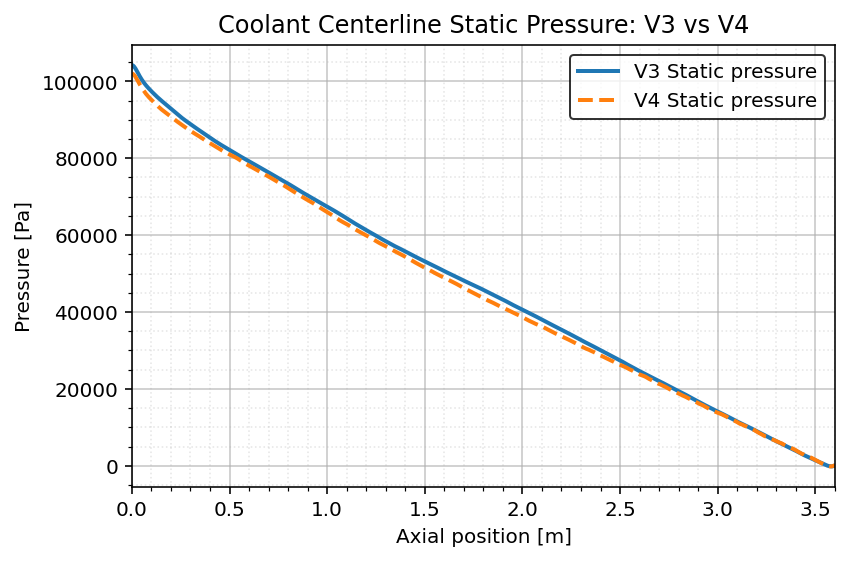
\includegraphics[width=0.48\linewidth]{figs/V3V4Pressure.png}
    \hfill
    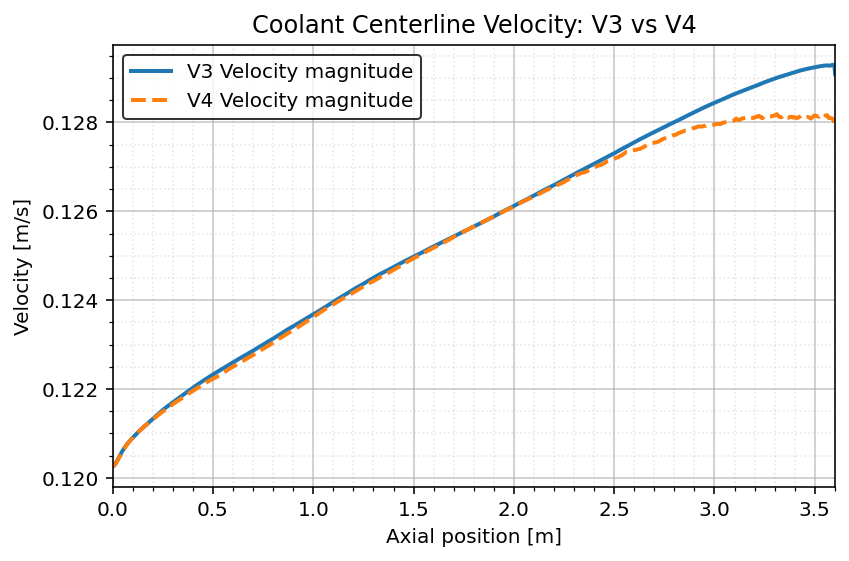
\includegraphics[width=0.48\linewidth]{figs/V3V4Velocity.png}
    \caption{Coolant centerline static pressure (left) and velocity (right) for V3 versus V4, confirming that the single-pin geometry reproduces the hydraulic behavior of the full 4-pin model.}
    \label{fig:v3v4_flow}
\end{figure}

The results indicate that the quantities of interest for this study---including wall temperature, outlet coolant temperature, and the radial temperature distribution---are preserved to acceptable accuracy when the 4-pin model is reduced to a single-pin representation. The major effect of transitioning from V4 to V5 is not hydraulic but solid-thermal: explicitly introducing cladding changes the radial temperature partitioning and allows the cladding surface temperature to be evaluated directly, while leaving the bulk coolant response comparatively unchanged. This validates the use of the V5 single-pin conjugate model as the authoritative CFD case for comparison against the analytical conduction model.

\begin{figure}[H]
    \centering
    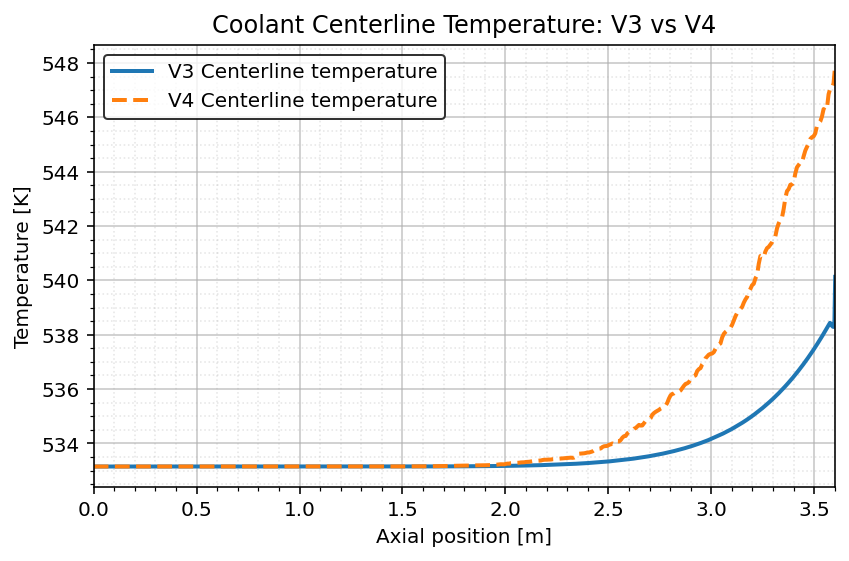
\includegraphics[width=0.75\linewidth]{figs/V3V4CenterTemp.png}
    \caption{Coolant centerline temperature for V3 versus V4. The differences are small and confined mainly near the outlet, further supporting the use of the single-pin approximation.}
    \label{fig:v3v4_coolT}
\end{figure}

After validating that the single-pin geometry reproduces the V3 four-pin Nusselt number and heat-transfer coefficient distributions, it was observed that reducing the model to a single pin slightly overpredicts the coolant temperature near the outlet. This behavior is consistent with expectations from Reynolds-averaged turbulence modeling: when geometric complexity is reduced, the resolved large-scale mixing between subchannels is diminished and the turbulence model must represent more of the cross-flow and swirl through its closure alone. In the full 4-pin geometry, small lateral pressure imbalances and geometric asymmetries promote cross-channel mixing that enhances convective heat removal and damps the axial growth of coolant temperature. In the symmetric single-pin domain, those mechanisms are suppressed, so the turbulence model predicts a somewhat weaker effective mixing and correspondingly higher bulk coolant temperature for the same power and mass flow. The resulting overprediction is modest and acceptable for this study, but it is important to recognize that the single-pin model is slightly conservative with respect to coolant temperature, especially toward the hot end of the channel.

% ============================================================
\subsection{Radial Temperature Maps from the Analytical Model}
\label{sec:radial-maps}
% ============================================================

To understand how material properties and the presence or absence of a gas gap affect temperature, the analytical model was evaluated across a power sweep from 15 to 60~W/g for several material and gap configurations. The resulting 2-D cross-section temperature maps show how fuel centerline temperature and cladding temperature increase with power.

\begin{figure}[H]
    \centering
    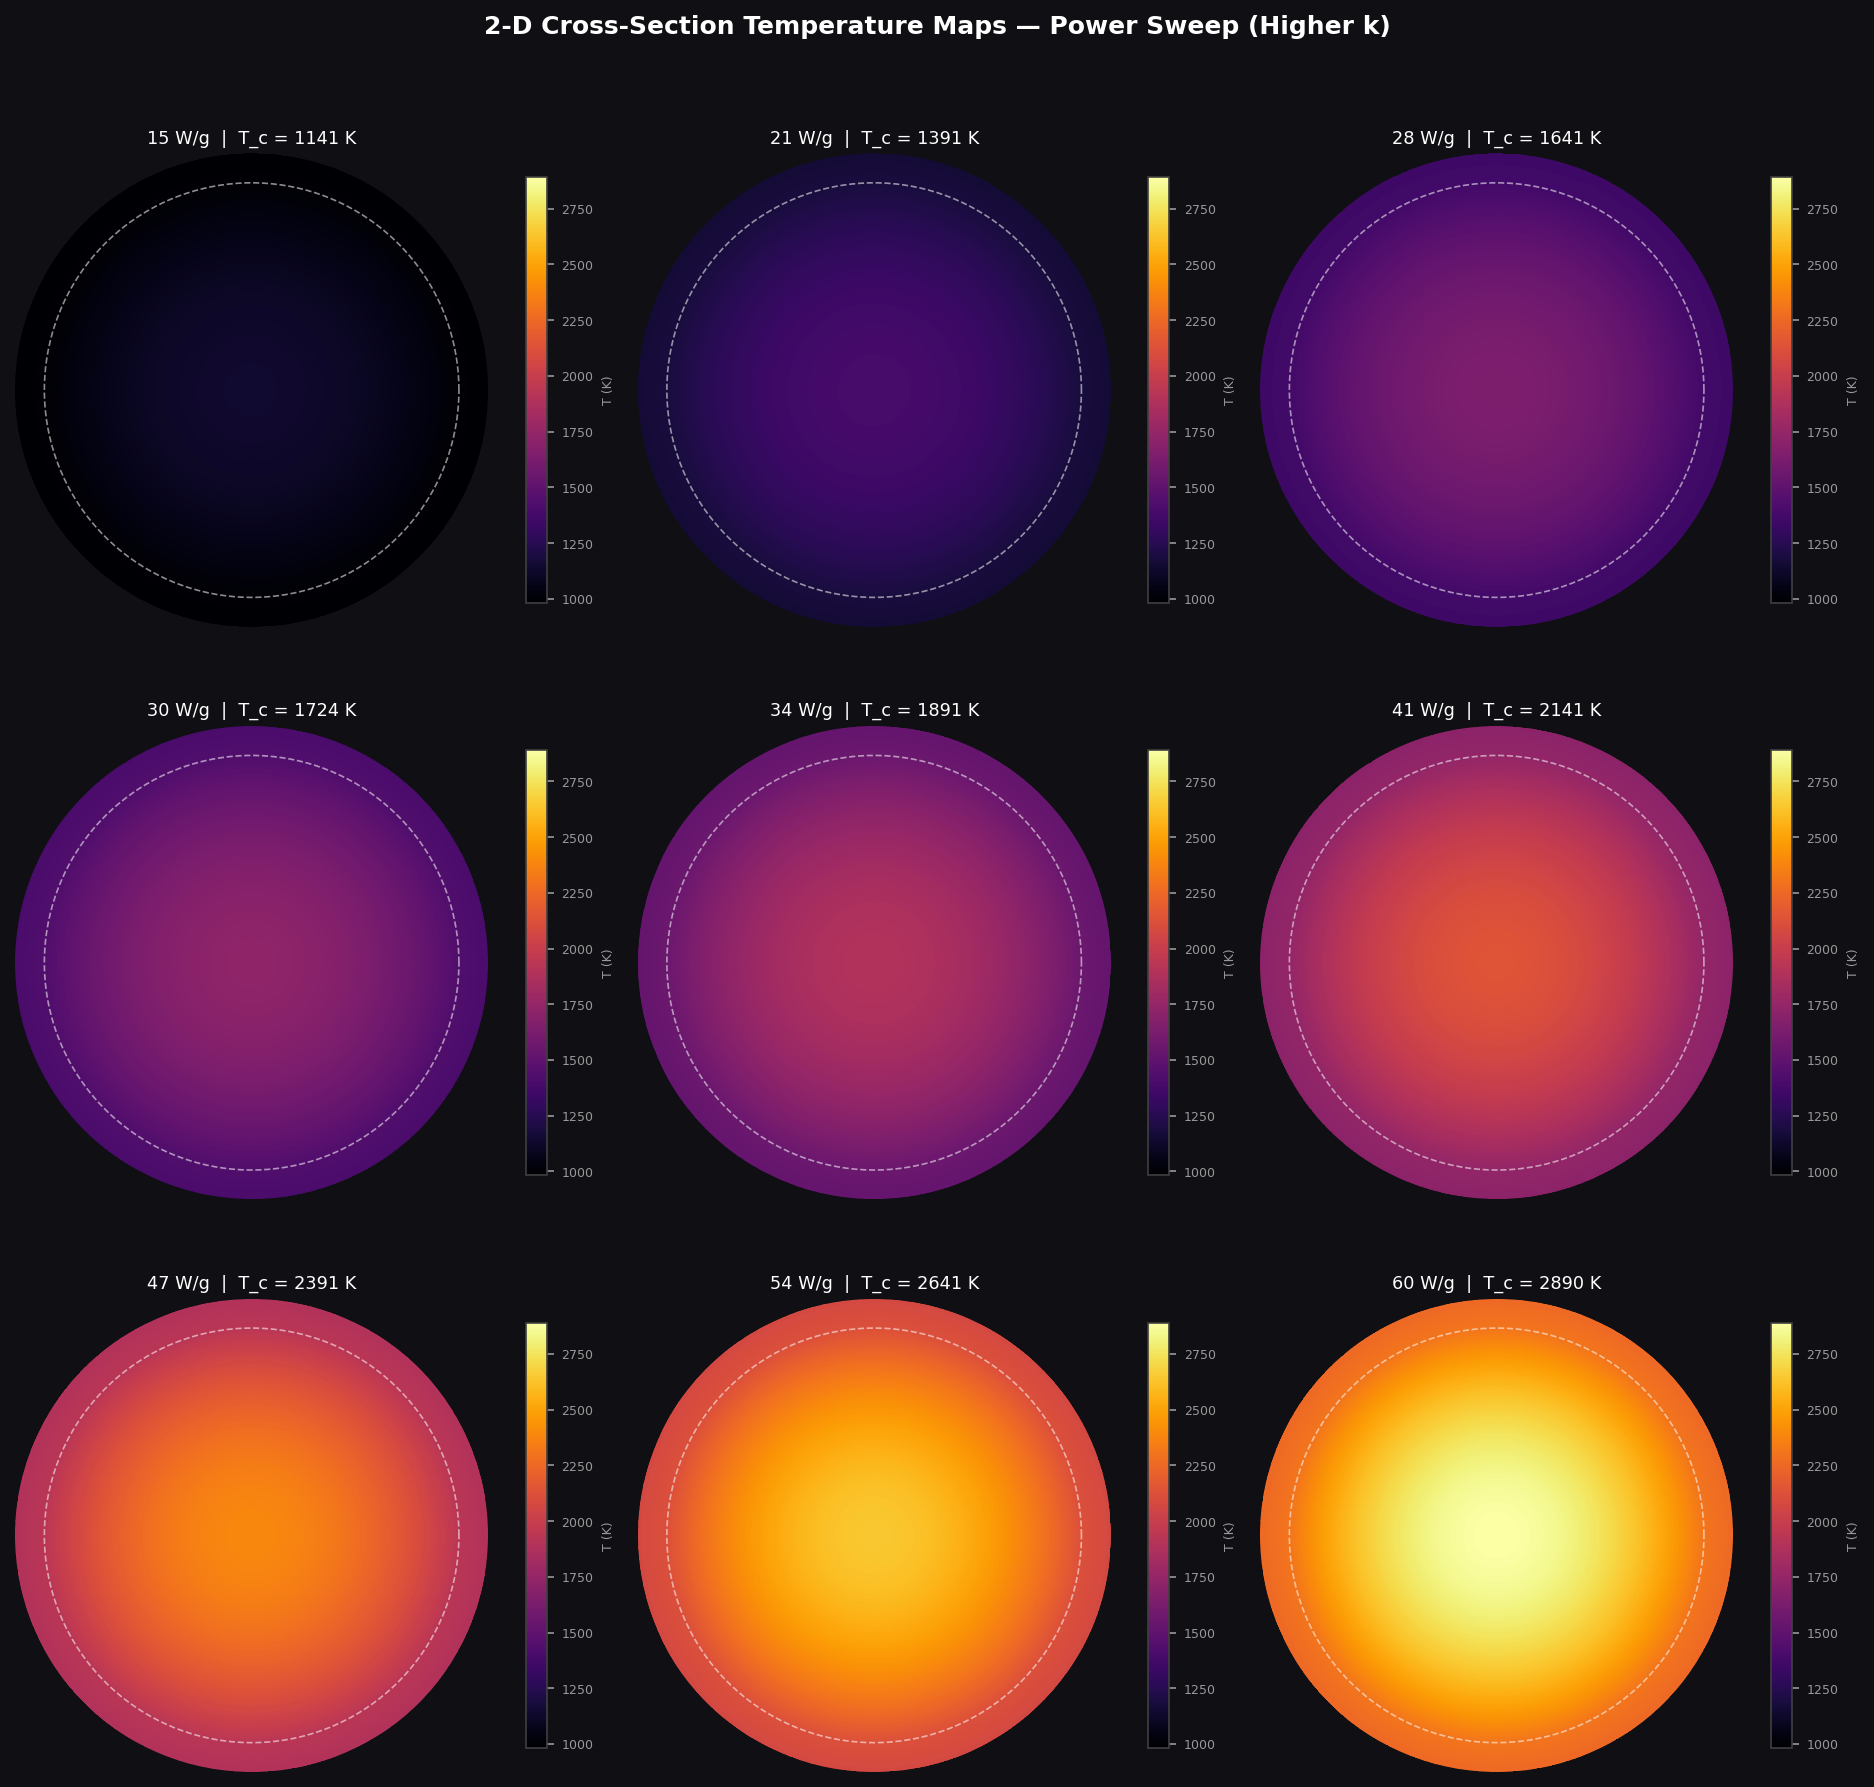
\includegraphics[width=0.55\linewidth]{figs/crosssection_grid_higher_k.png}
    \caption{2-D cross-section temperature maps for the power sweep using higher fuel and cladding thermal conductivities but no gas gap. Each panel shows the fuel centerline temperature \(T_c\) for a given specific power.}
    \label{fig:cs_higherk}
\end{figure}

\begin{figure}[H]
    \centering
    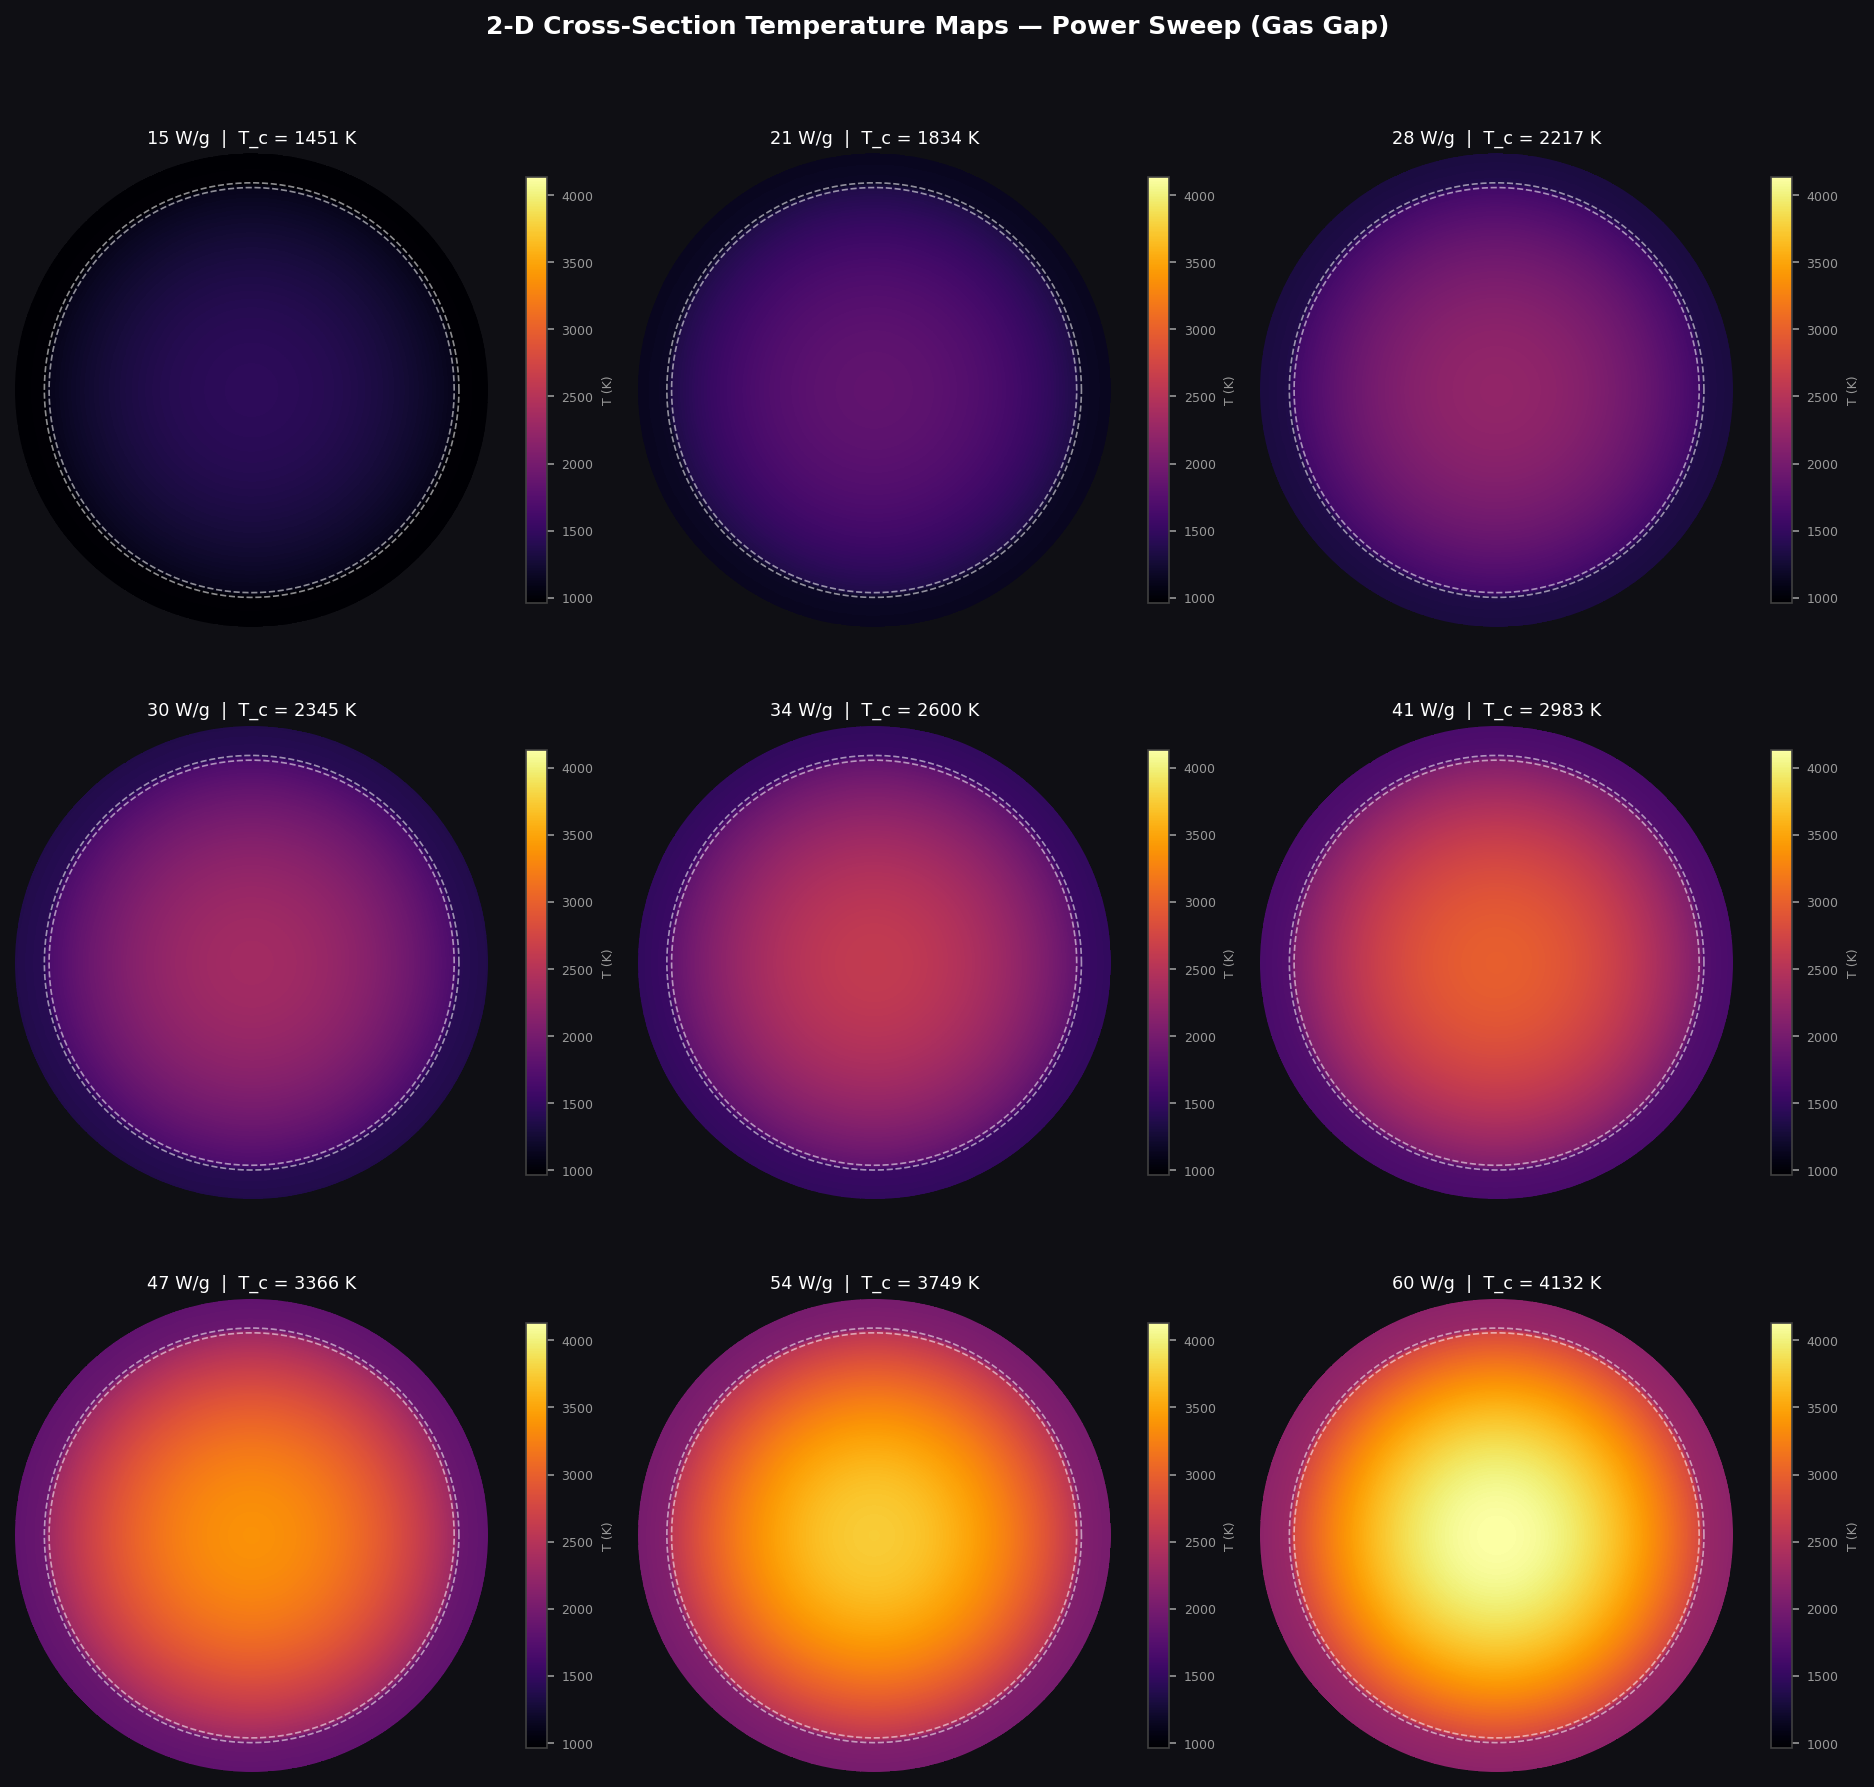
\includegraphics[width=0.5\linewidth]{figs/crosssection_grid_gg.png}
    \caption{2-D cross-section temperature maps for the power sweep including a gas gap with base thermal conductivities. The gas gap introduces an additional temperature drop between fuel and cladding, raising the fuel centerline temperature relative to the no-gap case.}
    \label{fig:cs_gg}
\end{figure}

\begin{figure}[H]
    \centering
    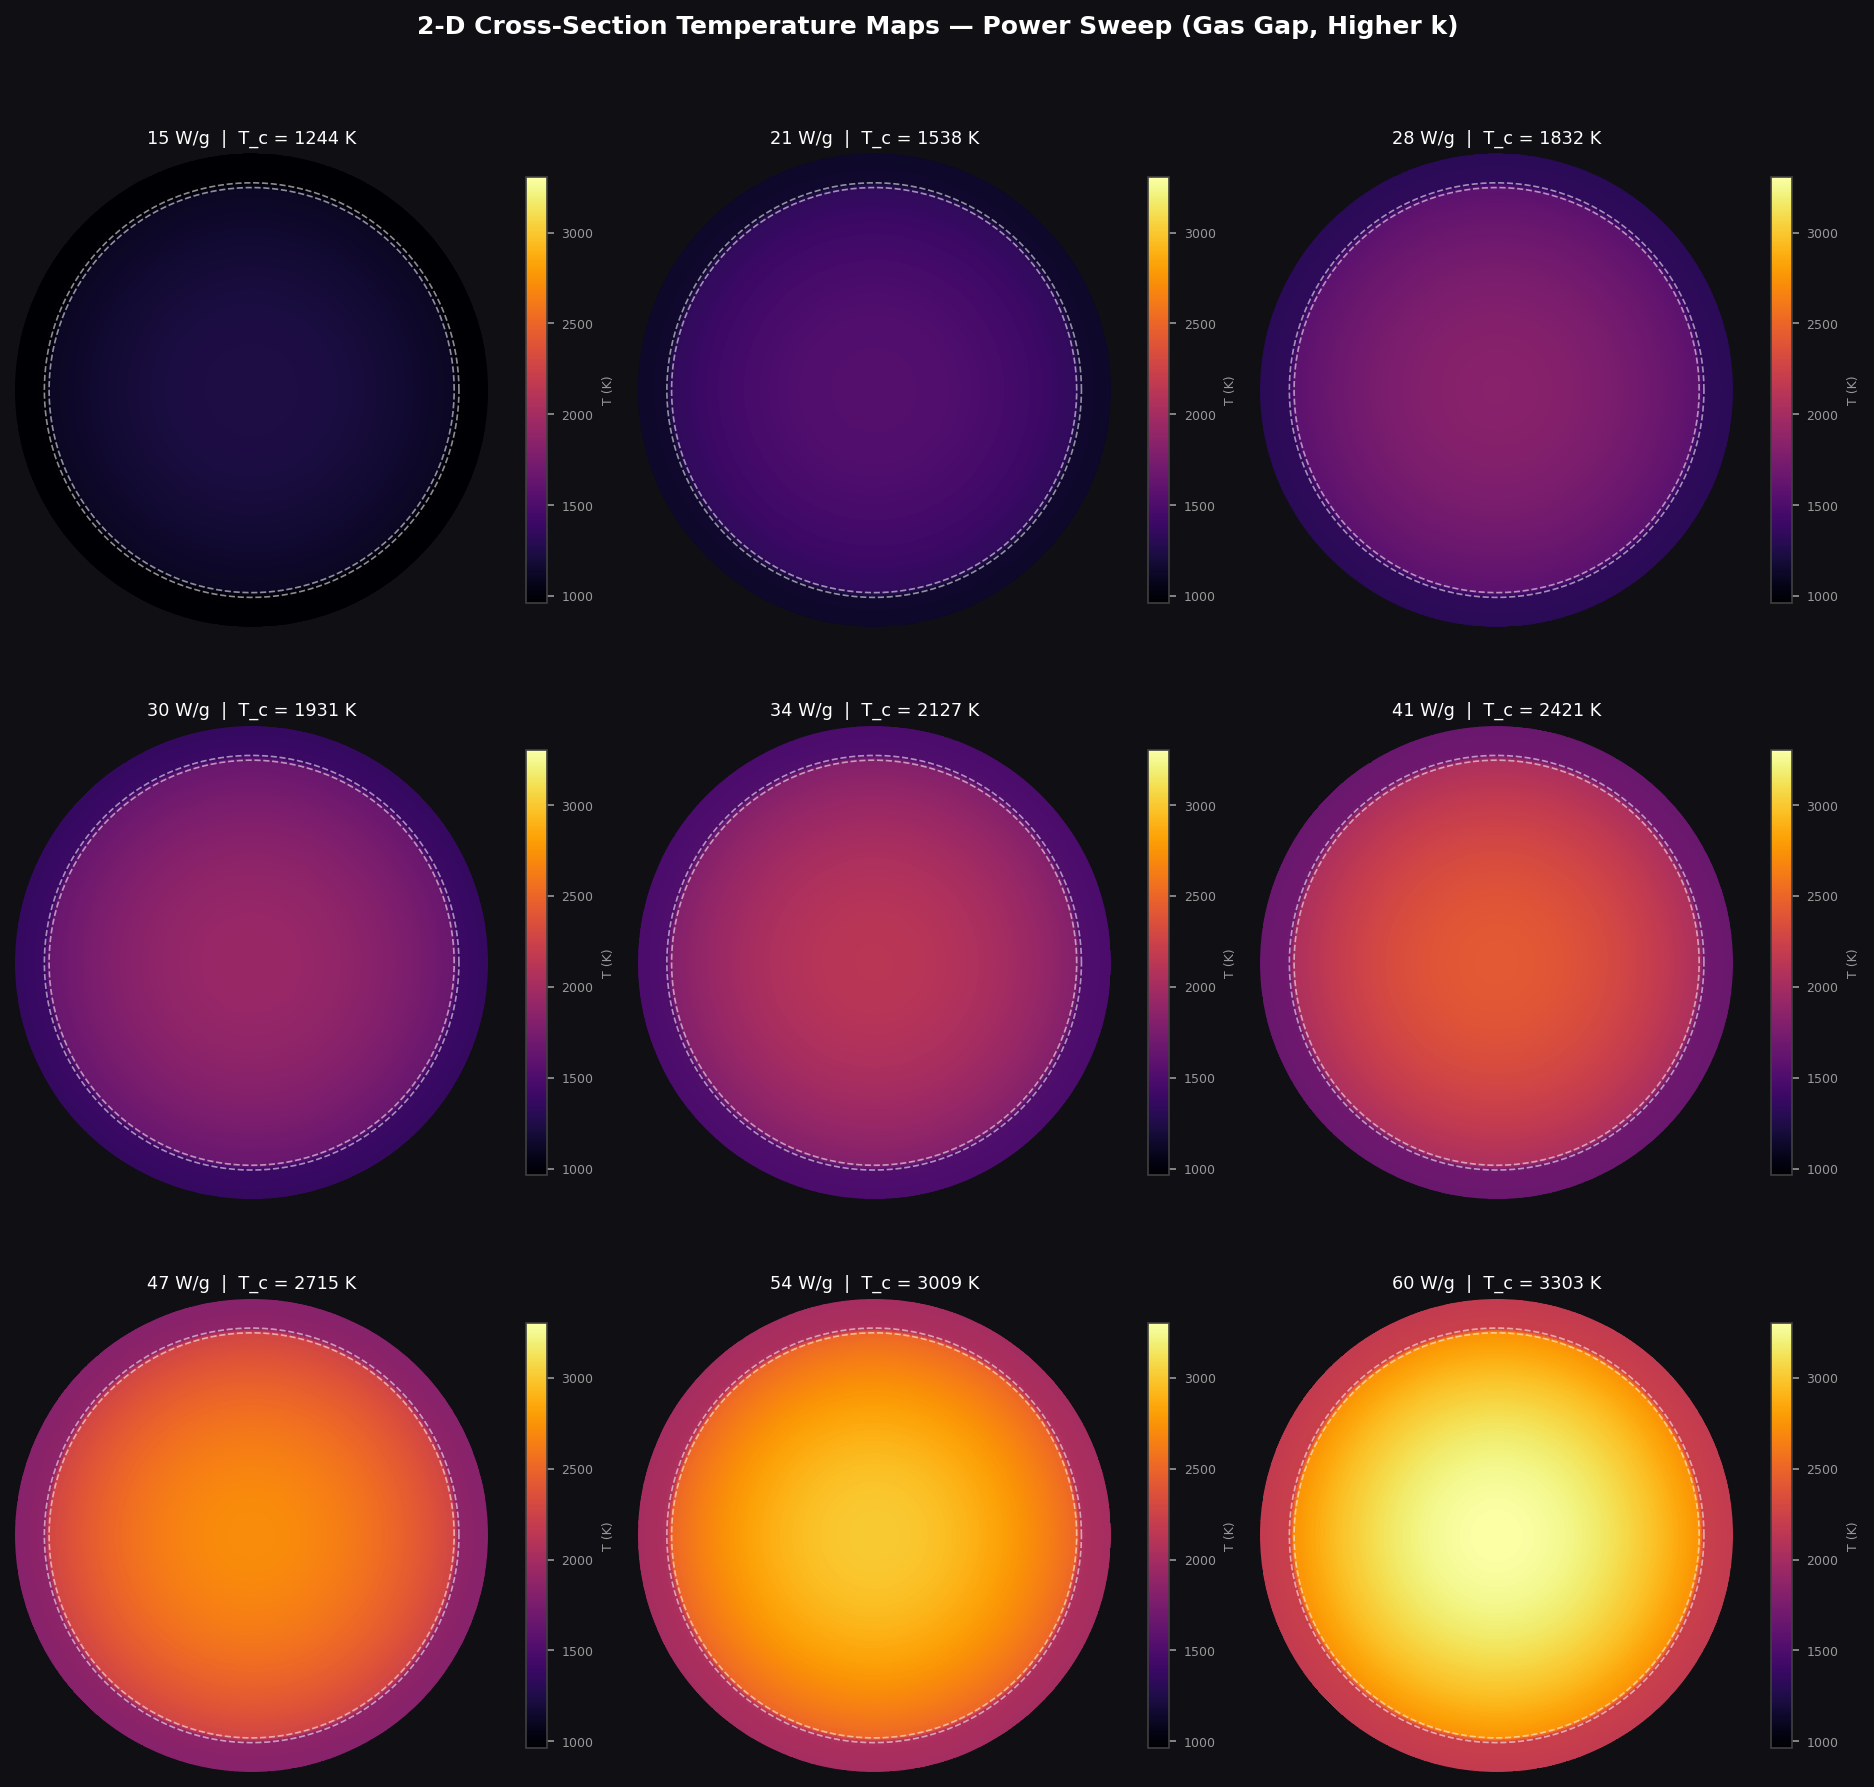
\includegraphics[width=0.5\linewidth]{figs/crosssection_grid_gg_k.png}
    \caption{2-D cross-section temperature maps for the power sweep including both a gas gap and higher fuel/cladding thermal conductivities.}
    \label{fig:cs_gg_higherk}
\end{figure}

\begin{figure}[H]
    \centering
    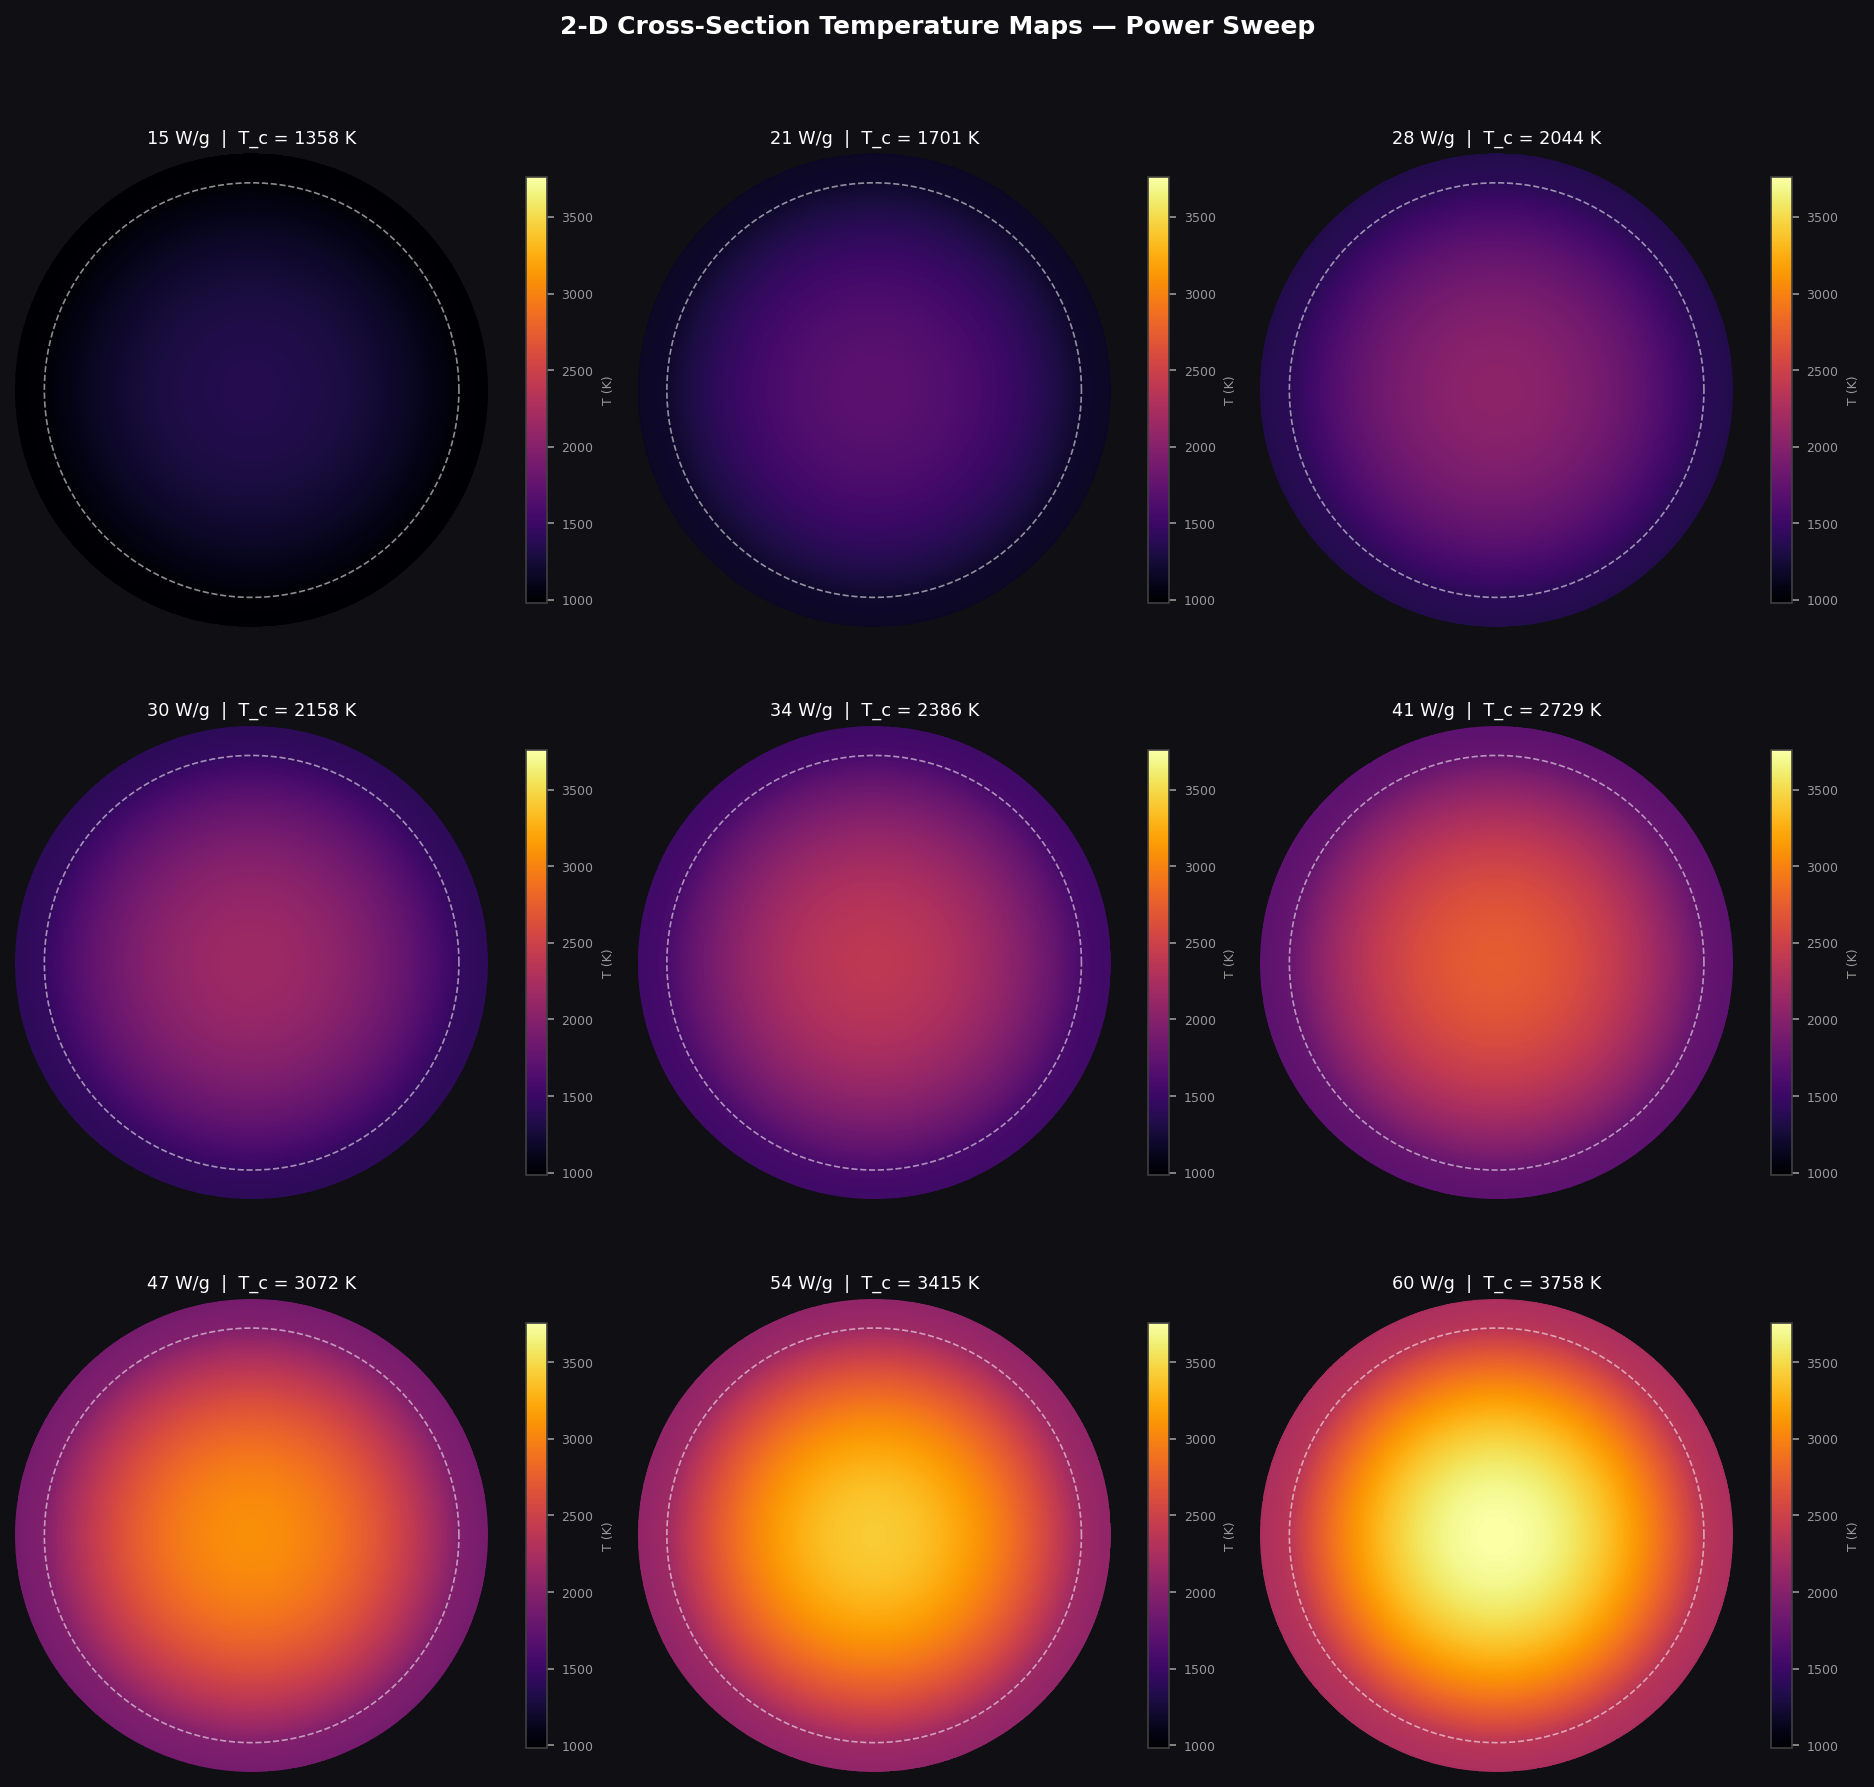
\includegraphics[width=0.5\linewidth]{figs/crosssection_grid.png}
    \caption{2-D cross-section temperature maps for the power sweep using the spent-fuel conductivity values and no gas gap, corresponding to the configuration most representative of the V5 CFD case.}
    \label{fig:cs_nominal}
\end{figure}

% ============================================================
\subsection{V5 Wall Quantities and \(y^+\) Distributions}
\label{sec:v5-wall}
% ============================================================

Beyond the area-averaged convergence metrics, spatial distributions of wall quantities provide additional insight into the thermal environment. Along the innermost edge of the fuel pin, the V5 solution shows Nusselt number, heat transfer coefficient, and wall heat flux that are relatively uniform over much of the heated length, with stronger variation only near the inlet.

\begin{figure}[H]
    \centering
    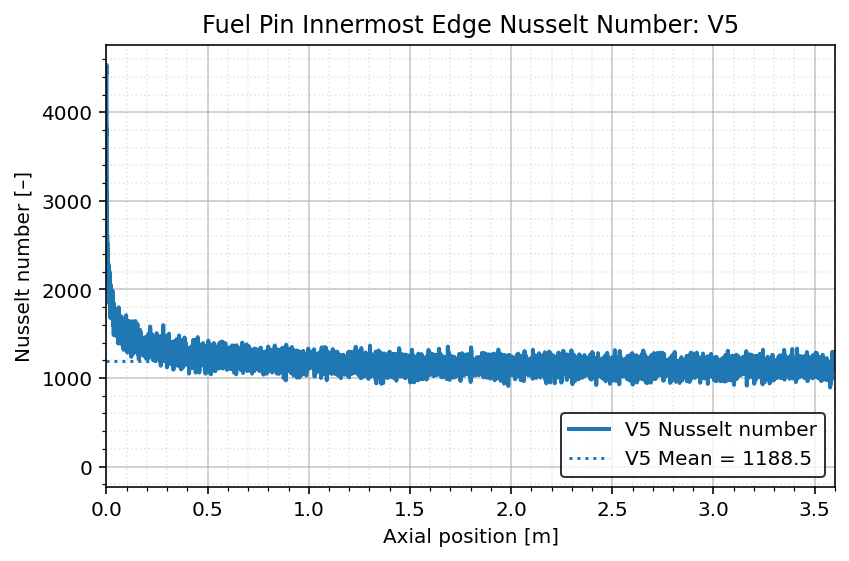
\includegraphics[width=0.58\linewidth]{figs/V5_CladNu.png}
    \caption{Fuel pin innermost-edge Nusselt number for case V5, with a mean value of approximately 1189.}
    \label{fig:v5_nusselt}
\end{figure}

\begin{figure}[H]
    \centering
    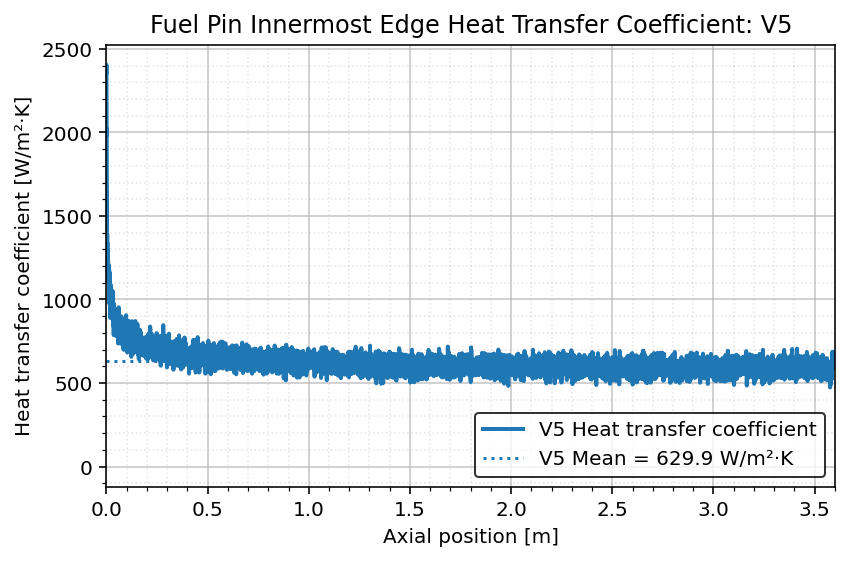
\includegraphics[width=0.6\linewidth]{figs/V5Clad_h.png}
    \caption{Fuel pin innermost-edge heat transfer coefficient for case V5, with a mean of about 630~W/m\(^2\)K.}
    \label{fig:v5_htc}
\end{figure}

\begin{figure}[H]
    \centering
    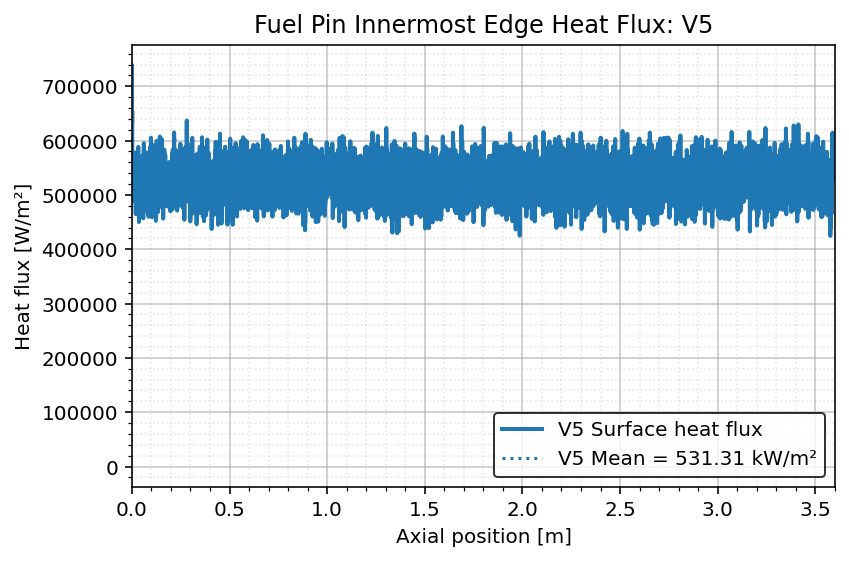
\includegraphics[width=0.6\linewidth]{figs/V5CladHeatFlux.png}
    \caption{Fuel pin innermost-edge surface heat flux for case V5, with a mean of about 531~kW/m\(^2\).}
    \label{fig:v5_q_axial}
\end{figure}

The \(y^+\) distribution along the same axial line remains in the desired near-wall–resolved regime for the SST \(k\)\(-\)\(\omega\) model. In wall-resolved simulations, \(y^+\) is typically maintained below about 5 (and ideally near 1) so that the viscous sublayer is directly resolved, whereas wall-modeled approaches place the first cell in the logarithmic layer with \(y^+ \gtrsim 30\) and rely on empirical wall functions for near-wall behavior. In this simulation the cladding-surface \(y^+\) values are clustered around 1–2, well within the wall-resolved range, so the SST \(k\)\(-\)\(\omega\) model is resolving the viscous sublayer rather than relying on wall functions for the heat-transfer prediction.

\begin{figure}[H]
    \centering
    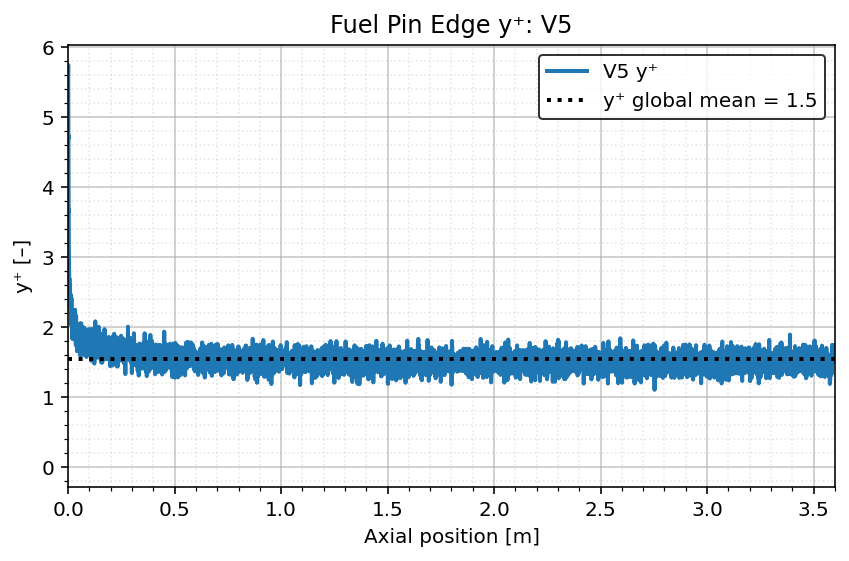
\includegraphics[width=0.6\linewidth]{figs/V5Yplus.png}
    \caption{Fuel pin edge \(y^+\) for case V5, with a global mean value of about 1.5, indicating that the first grid point lies within the viscous sublayer.}
    \label{fig:v5_yplus_axial}
\end{figure}

The corresponding cladding temperature along the same edge rises from roughly 780~K near the inlet to around 1170~K near the outlet.

\begin{figure}[H]
    \centering
    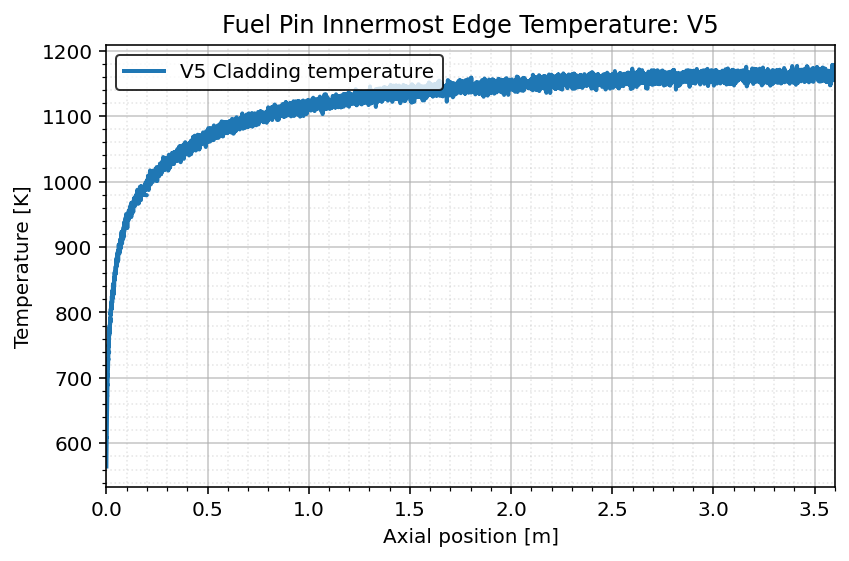
\includegraphics[width=0.6\linewidth]{figs/V5CladTemp.png}
    \caption{Fuel pin innermost-edge cladding temperature for case V5.}
    \label{fig:v5_cladT_axial}
\end{figure}

% ============================================================
\subsection{Regulatory and Design-Relevant Temperature Limits}
\label{sec:temp-limits}
% ============================================================

The purpose of the present thermal analysis is not only to report temperatures, but also to interpret them relative to accepted material limits. For Zircaloy-based cladding in water-cooled reactors, excessive cladding temperature is undesirable because it accelerates oxidation, hydriding, and mechanical degradation; regulatory guidance associated with light-water reactor safety analyses typically places strong attention on maintaining cladding temperatures well below high-temperature oxidation regimes. Likewise, for UO$_2$ fuel, the centerline temperature must remain below the melting range and should retain adequate margin to account for uncertainty in conductivity, cracking, and local peaking.

Regulatory limits provide a quantitative benchmark for interpreting these temperatures. For large-break loss-of-coolant accidents, 10~CFR~50.46(b)(1) specifies that the calculated maximum fuel element cladding temperature shall not exceed \cite{NRC_50_46}
\[
T_{\text{clad,peak}} \leq 2200~^{\circ}\text{F} \; (1204~^{\circ}\text{C}),
\]
together with auxiliary limits on cladding oxidation and hydrogen generation. Under normal operation and anticipated operational occurrences, the Standard Review Plan for fuel systems (NUREG--0800, Section~4.2) does not assign a single numeric centerline temperature limit; instead, it requires that UO$_2$ fuel remain below its melting temperature, and any rod that experiences centerline melting in postulated accidents is conservatively treated as failed for radiological analyses. In other words, the regulatory constraint for fuel is effectively a ``no centerline melting'' requirement during normal operation and AOOs, rather than a fixed temperature threshold.

\begin{figure}[H]
    \centering
    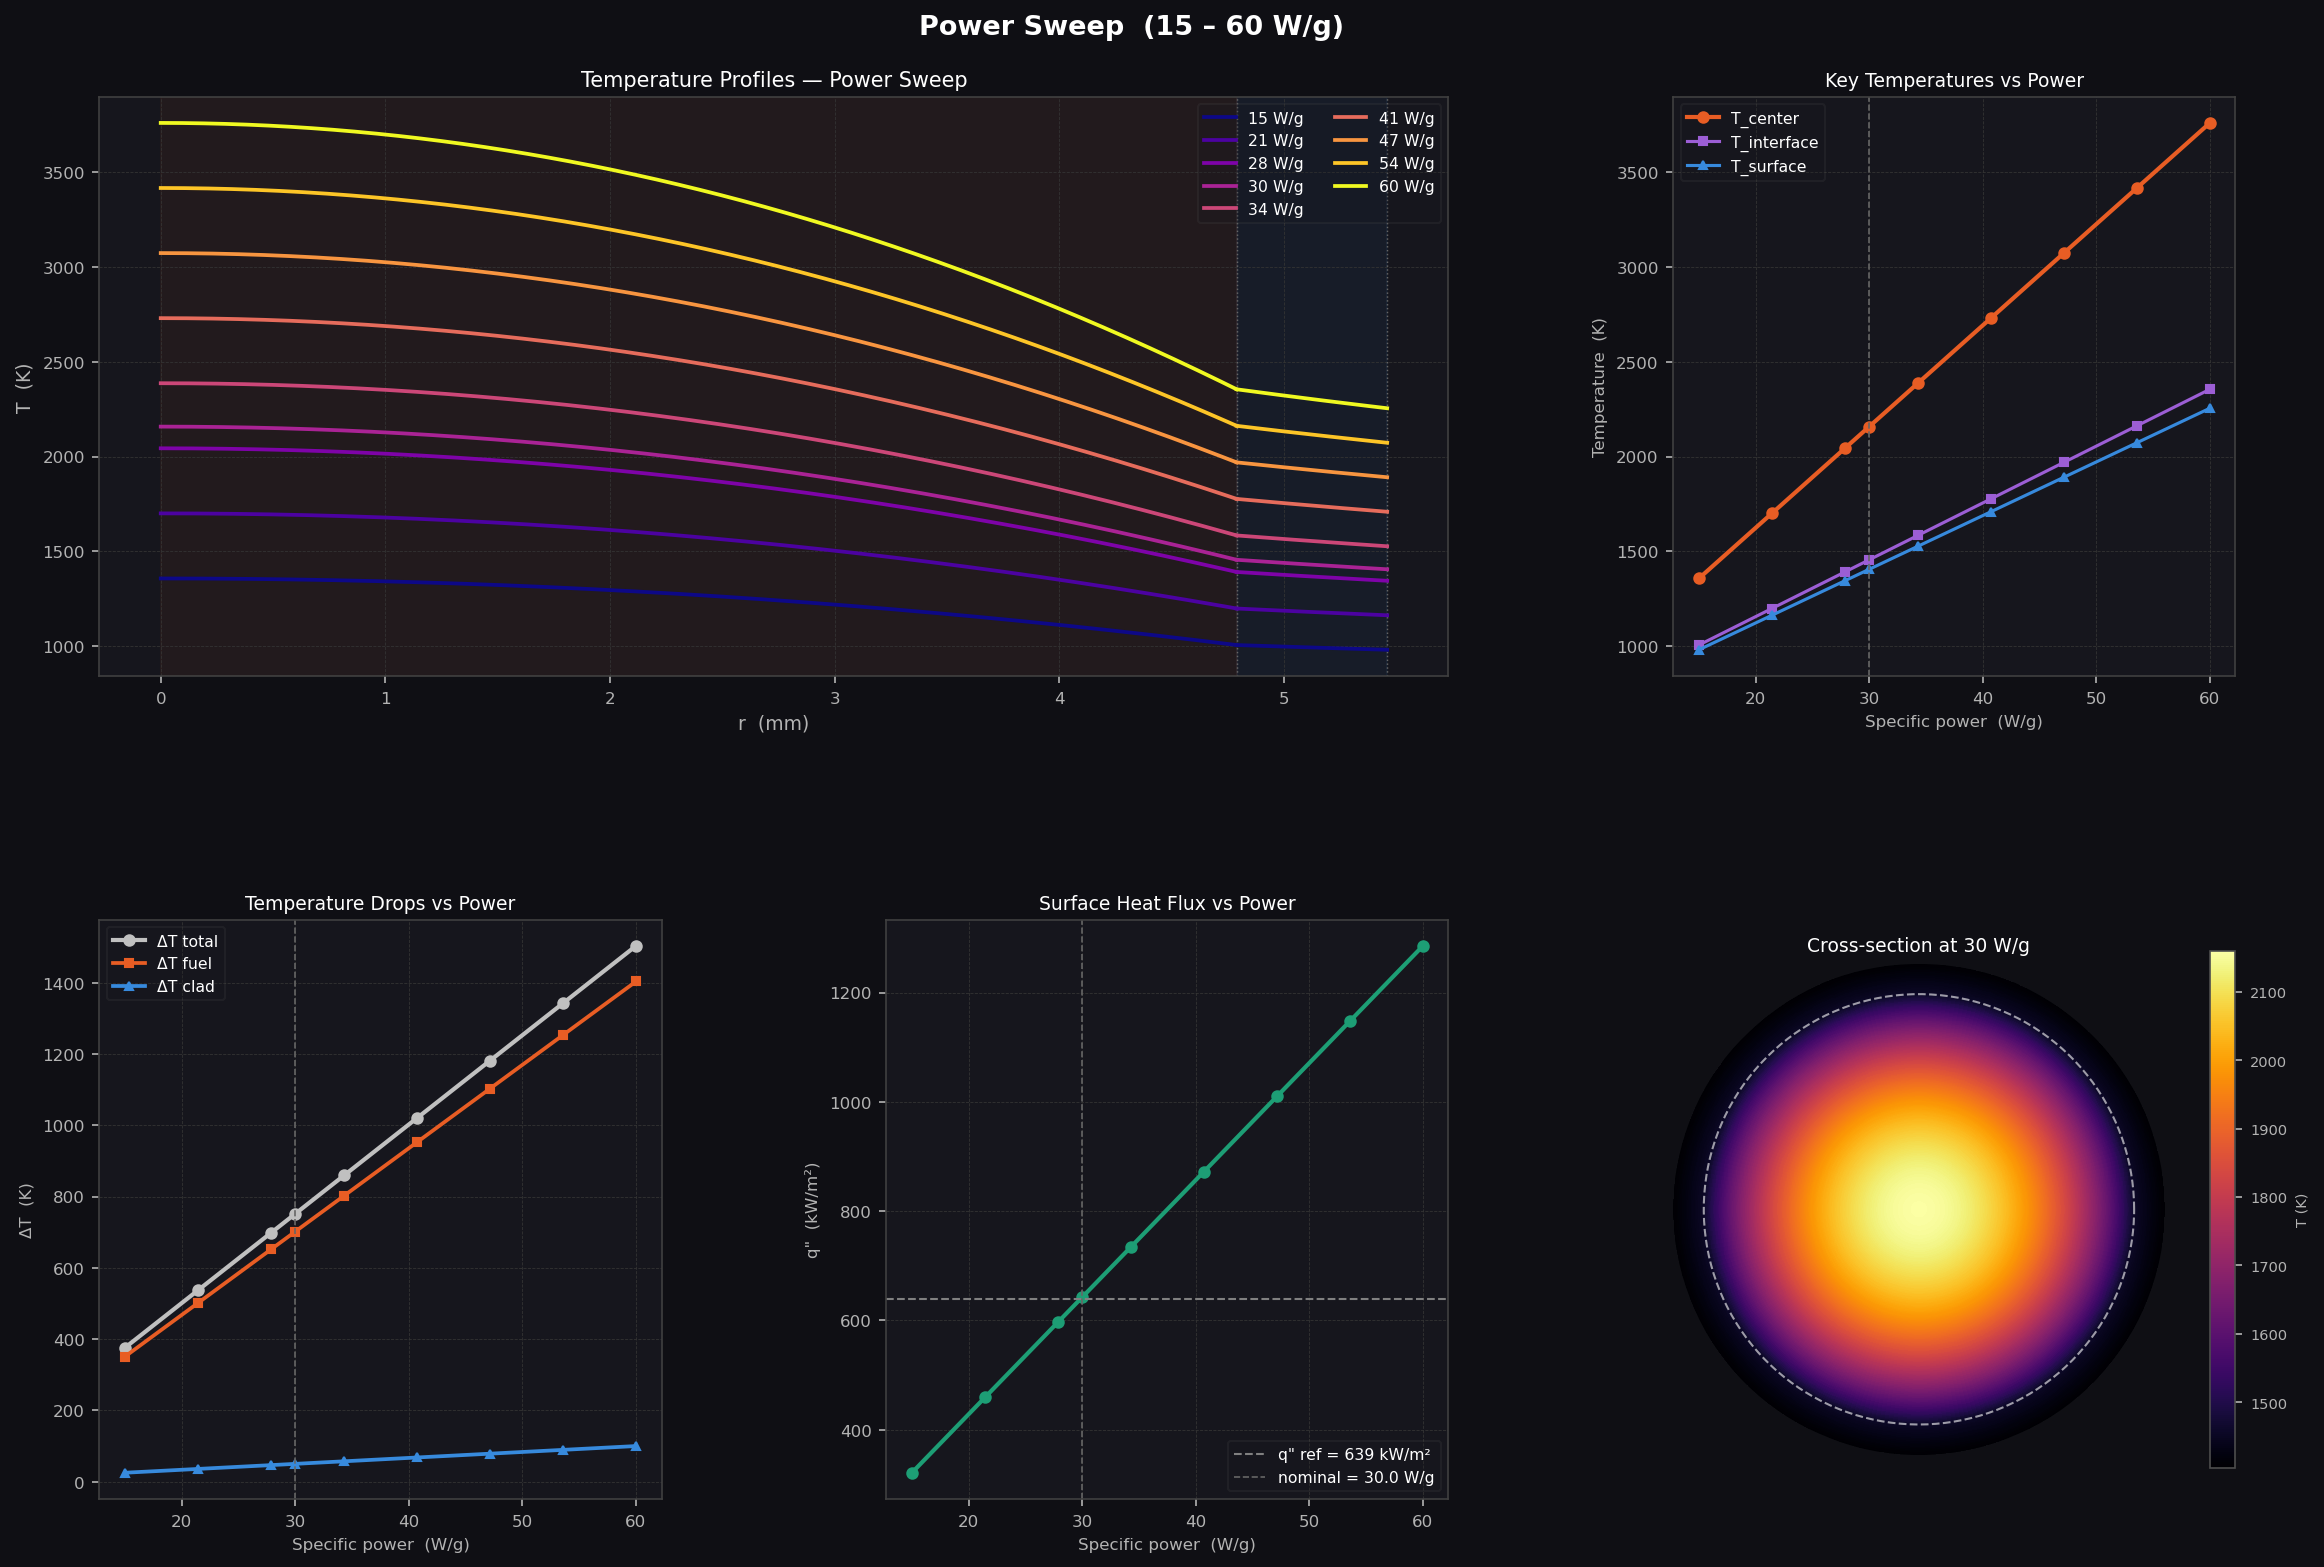
\includegraphics[width=0.90\linewidth]{figs/power_sweep.png}
    \caption{Fuel centerline and cladding surface temperature as functions of specific power for the average channel. The nominal design point at 30~W/g is highlighted for comparison against regulatory cladding and fuel temperature constraints.}
    \label{fig:temp_vs_power}
\end{figure}

Figure~\ref{fig:temp_vs_power} summarizes the behavior of the LBR average channel over the 15--60~W/g power sweep by plotting both cladding surface temperature and fuel centerline temperature versus specific power. At the nominal 30~W/g design point, the CFD-calibrated analytical model predicts a maximum-channel cladding temperature of approximately 1250~K, which lies below the 1204~$^{\circ}$C peak-cladding temperature limit. The corresponding fuel centerline temperature is approximately 1900~K, below the UO$_2$ melting range (2800~K - 2900~K), however providing insubstantial margin to the ``no melting'' criterion when the power peaking factor is applied (resulting in greater than 60 W/g power density which can be seen on the figure above). However, when the same sweep is interpreted with the power peaking factor applied to obtain a hot-channel estimate, the cladding and centerline temperatures are higher than their respective constraints. This illustrates that the thermal constraint on the LBR concept is driven less by the average 30~W/g channel and more by the combination of elevated peaking, degraded spent-fuel conductivity, and weak convective heat transfer associated with the 6~cm lattice pitch.

In the LBR concept, the average channel at 30~W/g may remain thermally manageable when interpreted through the CFD-calibrated analytical model. However, the corresponding hot-channel condition obtained by multiplying by the power peaking factor can drive cladding and centerline temperatures much higher. This is the central thermal design concern of the reactor: not the average channel itself, but the combination of wide pitch, low mass flux, degraded spent-fuel conductivity, and elevated PPF required by the neutronics-driven loading strategy.

% % ============================================================
% \subsection{Implications for Design Improvement}
% \label{sec:th-improvement}
% % ============================================================

% MOVED TO VIABILITY SECTION

\clearpage

% ============================================================
% MATERIALS
% ============================================================
\section{Materials Design and Analysis (R. Imam)}
\label{sec:Materials}
The structural integrity of fuel and cladding materials under irradiation, thermal cycling, and corrosion is a critical constraint in reactor design. Neutronics performance controls reactivity and the effective use of fuel; however, material damage affects safety margins and operational lifetime. This section of the report presents the use of a multiphysics modeling framework to simulate fuel-cladding performance in the Last Breath Reactor (LBR) with the primary focus being on thermal gradients, stress evolution and damage mechanisms.

\subsection{Modeling Framework: Use of MOOSE}
The Multiphysics Object-Oriented Simulation Environment (MOOSE), developed by Idaho National Laboratory, was used to model the coupled thermomechanical and fracture behavior of the fuel–cladding system. MOOSE enables the solution of strongly coupled nonlinear partial differential equations using the finite element method within a modular, extensible framework.

MOOSE was chosen primarily for its ability to simulate coupled heat conduction and solid mechanics within a single simulation environment. Moreover, MOOSE supports custom material models, including corrosion-induced property degradation and eigenstrain contributions. This was essential, as it enabled the simulation of accurate estimates of material property degradation caused by the extreme thermo-mechanical stresses that PWR fuel generally experiences during heating and cooling. Afterward, a realistic variant of a damaged spent fuel pin was simulated through a reheating cycle in the Last Breath Reactor to test its survivability and failure limits.


\subsection{Governing Physics and Equations}
Using the Multiphysics framework of MOOSE the thermo-mechanical behavior of the fuel cladding system was modeled. The coupled framework integrated heat conduction, solid mechanics, creep deformation, corrosion and fracture. Below are the governing equations and corresponding assumptions that modeled this simulation

\paragraph{Heat Conduction}
The temperature distribution within the fuel pellet is governed by the heat conduction equation:
\begin{equation}
    \rho c_p\frac{\partial T}{\partial t}=\nabla\cdot\left(k_{\mathrm{eff}}\nabla T\right)+Q
\end{equation}
Due to volumetric heat generation from fission, strong radial temperature gradients develop, with peak temperatures occurring at the fuel centerline. Heat transfer occurs radially outwards towards the cladding where a convective heat flux boundary condition is established. As for the cooling phase, the heat generation term is reduced to zero.

\paragraph{Solid Mechanics}
Mechanical equilibrium is described by:
\begin{equation}
    \nabla\cdot \sigma + b =0
\end{equation}

where $\sigma$ is the Cauchy stress tensor (Pa), and $b$ represents body forces, which are assumed to be negligible in this study.

Since the scope of these simulations covers a 2D axisymmetric radial geometry, the stresses that make up the stress tensor are the radial and hoop stresses.

The hoop stress ($\sigma_\theta$) is described by:
\begin{equation}
    \sigma_\theta = \sigma_\theta(r)
\end{equation}

where:
\begin{itemize}
	\item $\sigma_\theta$ is the hoop (circumferential) stress (Pa),
	\item $r$ is the radial position (m).
\end{itemize}

The radial stress ($\sigma_r$) is described by:
\begin{equation}
    \sigma_r = \sigma_r(r)
\end{equation}

where:
\begin{itemize}
	\item $\sigma_r$ is the radial stress (Pa),
	\item $r$ is the radial position within the fuel--cladding system (m).
\end{itemize}

The total strain ($\varepsilon$) is decomposed as:
\begin{equation}
    \varepsilon = \varepsilon_e + \varepsilon_{th} + \varepsilon_{cr}\quad ,
\end{equation}
where $\varepsilon_e$ is the elastic strain, $\varepsilon_{th}$ is the thermal strain, and $\varepsilon_{cr}$ is the creep strain.

Here, the elastic response follows a linear isotropic Hooke's Law
\begin{equation}
    \varepsilon_r = \frac{1}{E} \left( \sigma_r - \nu \sigma_\theta \right)
\end{equation}

\begin{equation}
    \varepsilon_\theta = \frac{1}{E} \left( \sigma_\theta - \nu \sigma_r \right)
\end{equation}

where:
\begin{itemize}
	\item $\varepsilon_r$, $\varepsilon_\theta$ are the radial and hoop strains (-),
	\item $\sigma_r$, $\sigma_\theta$ are the radial and hoop stresses (Pa),
	\item $E$ is Young’s modulus (Pa),
	\item $\nu$ is Poisson’s ratio (-).
\end{itemize}

while thermal strain is computed by:
\begin{equation}
    \varepsilon_{th}=\alpha\left(T-T_\text{ref}\right)\mathbf{I}
\end{equation}

Where,  $\alpha$ is the coefficient of thermal expansion (1/K), $T_\text{ref}$ is the reference temperature, and $\mathbf{I}$ is the identity tensor. The mismatch in expansion rates between fuel and cladding induces stresses, leading to pellet-clad interaction (PCI).

Meanwhile, the creep strain is modeled by a Norton-type power law creep formulation with Arrhenius temperature dependence:

\begin{equation}
    \dot{\varepsilon}_{cr}=A\sigma_{\text{vm}}^{n}\exp{\left(-\frac{Q}{RT}\right)}
\end{equation}

where:
\begin{itemize}
	\item ${\dot{\varepsilon}}_{cr}$ is the creep strain rate (1/s),
	\item $A$ is a material constant,
	\item $\sigma_{vm}$ is the Von Mises equivalent stress (Pa),
	\item $n$ is the stress exponent,
	\item $Q$ is the activation energy (J/mol),
	\item $R$ is the universal gas constant (J/mol$\cdot$K),
	\item $T$ is temperature (K).
\end{itemize}

The Von Mises stress, $\sigma_{vm}$, is an equivalent stress derived from the distortion energy in a material. In this study, it is an overall stress state contributed by the hoop and radial stresses that drives the creep mechanism in the material.

\begin{equation}
    \sigma_{\text{vm}} = \sqrt{\sigma_r^2 - \sigma_r \sigma_\theta + \sigma_\theta^2}
\end{equation}

where:
\begin{itemize}
	\item $\sigma_{\text{vm}}$ is the Von Mises equivalent stress (Pa),
	\item $\sigma_r$ is the radial stress (Pa),
	\item $\sigma_\theta$ is the hoop (circumferential) stress (Pa).
\end{itemize}

This formulation captures the strong dependence of creep on both stress and temperature, making it particularly important under high-temperature conditions experienced in the Last Breath Reactor (LBR) cycle.

The overall thermal strain and stress drive the phase field to initiate crack propagation, which is modeled by Allen-Cahn:

\begin{equation}
    \frac{\partial\phi}{\partial t}=-L\frac{\delta F}{\delta\phi}\quad,
\end{equation}

where $\phi$ is the phase-field damage variable (0 = intact, 1 = fully fractured), $L$ is a mobility parameter, and $F$ is the total free energy functional.

Although this model was not used in the final Last Breath Reactor simulation, it was necessary to use it in the primary heating cycle to induce cracks in the fuel which would degrade the thermal conductivity. The model has also partially, i.e. at a small portion of the entire cycle timeline, been used in the LBR cycle to check for cladding rupture. The crack propagation is strongly coupled to thermal stress fields generated during reactor operation.

Meanwhile, for the cladding that is exposed to water for such a long time, a Arrhenius, temperature coupled corrosion model was applied

\begin{equation}
    x\left(t\right)=k_0\exp{\left(-\frac{Q}{RT}\right)}t^n
\end{equation}

where:
\begin{itemize}
	\item $x(t)$ is oxide thickness (m),
	\item $k_0$ is a rate constant,
	\item $Q$ is activation energy,
	\item $T$ is temperature,
	\item $n$ is a time exponent.
\end{itemize}

With a property degradation model of,
\begin{equation}
    D\left(T,t\right)=\operatorname{D}_0\exp{\left(-A\exp{\left(-\frac{\operatorname{Q}}{RT}\right)}t\right)}
\end{equation}

Where, D is a parameter such as conductivity, stiffness (Young’s modulus) etc. is degraded based on the corrosion.

\subsection{Modeling Assumptions}

To ensure computational tractability while capturing the dominant physical behavior, the following assumptions are made:
\begin{itemize}
    \item The problem is modeled in a 2D axisymmetric geometry, representing a radial cross-section of the fuel rod.
    \item Heat generation is applied only within the fuel region and is spatially uniform.
    \item Decay heat is neglected as it makes up about 7\% of the total reactor heat generation and decreases with time. 
    \item Mechanical behavior is quasi-static, with inertial effects neglected.
    \item Irradiation-induced swelling and fission gas release are neglected. However, for this model, these effects were ignored due to a relatively shorter operational cycle length for which the irradiation damage would be secondary to the thermo-mechanical damages \cite{Sweet2016BISONProperties}.%(Oak Ridge National Laboratory, Radiation Effects in Structural Materials, ORNL Report, 2017.: https://info.ornl.gov/sites/publications/files/Pub69721.pdf).
    \item Corrosion is temperature-driven and occurs only on exposed cladding surfaces.
    \item Material properties degrade as functions of temperature, stress, and damage but remain isotropic.
    \item The fuel gas gap was neglected in the simulations to ensure a tight configuration which occurs generally at the end of cycle for most PWR fuel \cite{Barrett2012AdvancedStudy}.%(U.S. Department of Energy, Advanced LWR Nuclear Fuel Cladding System Development Trade Study, 2012. [Online]. Available: https://www.energy.gov/ne/articles/advanced-lwr-nuclear-fuel-cladding-system-development-trade-study). 
\end{itemize}


These assumptions allow the model to focus on the dominant coupling between thermal gradients, stress evolution, creep deformation, corrosion, and fracture, which govern the structural integrity of the fuel–cladding system under LBR conditions.

\subsection{Primary heating cycle}
Simulations were modeled using the fuel material properties from Three Mile Island (TMI) Unit 1. The fuel was heated to a volumetric heat of 271 MW/m$^3$ under convective heat-flux boundary conditions.
Simulation results indicate the presence of strong radial temperature gradients within the fuel pellet, with centerline temperatures exceeding 1100 K and outer surface temperatures near 480 K. This is a characteristic behavior of UO$_2$ fuel due to the fuel having a relatively lower thermal conductivity than the cladding, which limits radial heat transport and this becomes the primary driver of stress development within the system.

\begin{figure}[H]
    \centering
    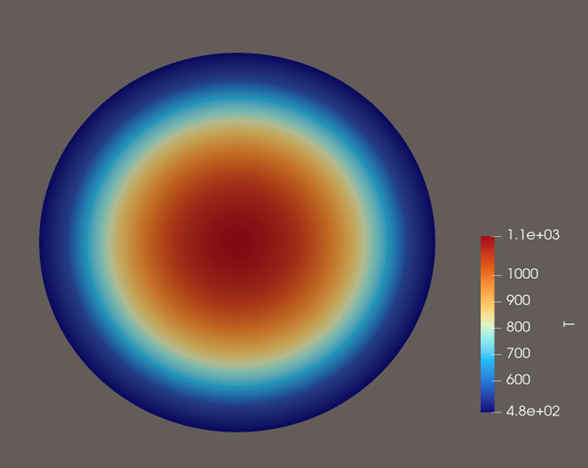
\includegraphics[width=0.5\linewidth]{figs/radial_heat_first_cycle.png}
    \caption{Radial Temperature profile in Kelvins for the first heating cycle at steady state.}
    \label{fig:placeholder}
\end{figure}

At the same time, the induced thermal expansion generates a significant mechanical stress due to the containment by the cladding. With the hoop stress profile it can be observed that there are compressive stresses in the fuel centerline and tensile stresses near the fuel-cladding interface. This is a direct consequence of the differential thermal expansion where the hot fuel expands relatively a lot more than the cooler cladding that leads to PCI.

\begin{figure}[H]
    \centering
    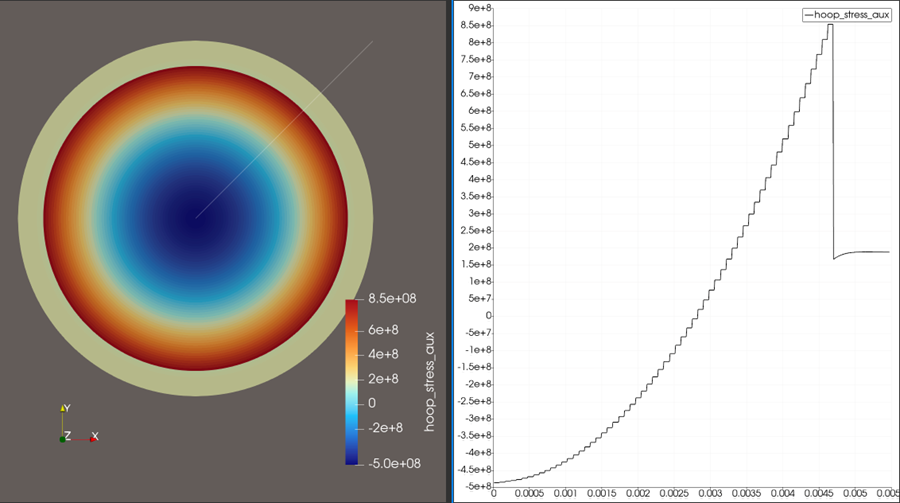
\includegraphics[width=0.6\linewidth]{hoopstress-ss.png}
    \caption{Hoop stress (Pa) at steady state }
    \label{fig:placeholder}
\end{figure}

The radial stress on the other hand helps monitor the compressive contact pressure between the cladding and the fuel. A high value at the fuel cladding interface during PCI indicates a high risk of plastic deformation and creep.

\begin{figure}[H]
    \centering
    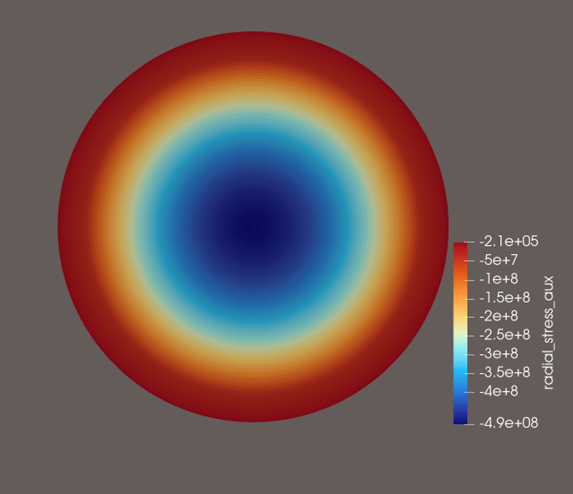
\includegraphics[width=0.5\linewidth]{figs/radial-stress-ss.png}
    \caption{The radial stress profile (Pa) at steady state.}
    \label{fig:placeholder}
\end{figure}
The hoop stresses and the radial stresses together contribute an overall stress state that yields the Von Mises stress, which mainly drives the creep mechanism that takes place during the cycle. This stress has a high value in the center of the fuel, which due to its ceramic properties undergoes constant deformation throughout the cycle. For the cladding on the other hand the stress is comparatively lower but still high enough to drive creep in the cladding region. As a result, the cladding is quite susceptible to failure by creep when it is eventually reheated in the LBR cycle.

\begin{figure}[H]
    \centering
    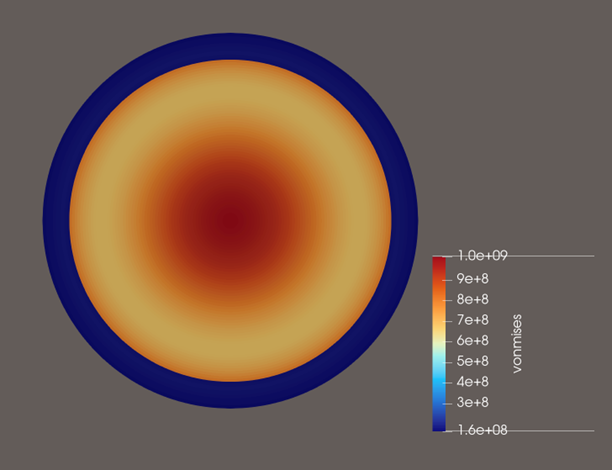
\includegraphics[width=0.5\linewidth]{figs/von-mises-ss-tmi1.png}
    \caption{Von Mises Stress profile at steady state during the operation of TMI-1.}
    \label{fig:placeholder}
\end{figure}

\begin{figure}[H]
    \centering
    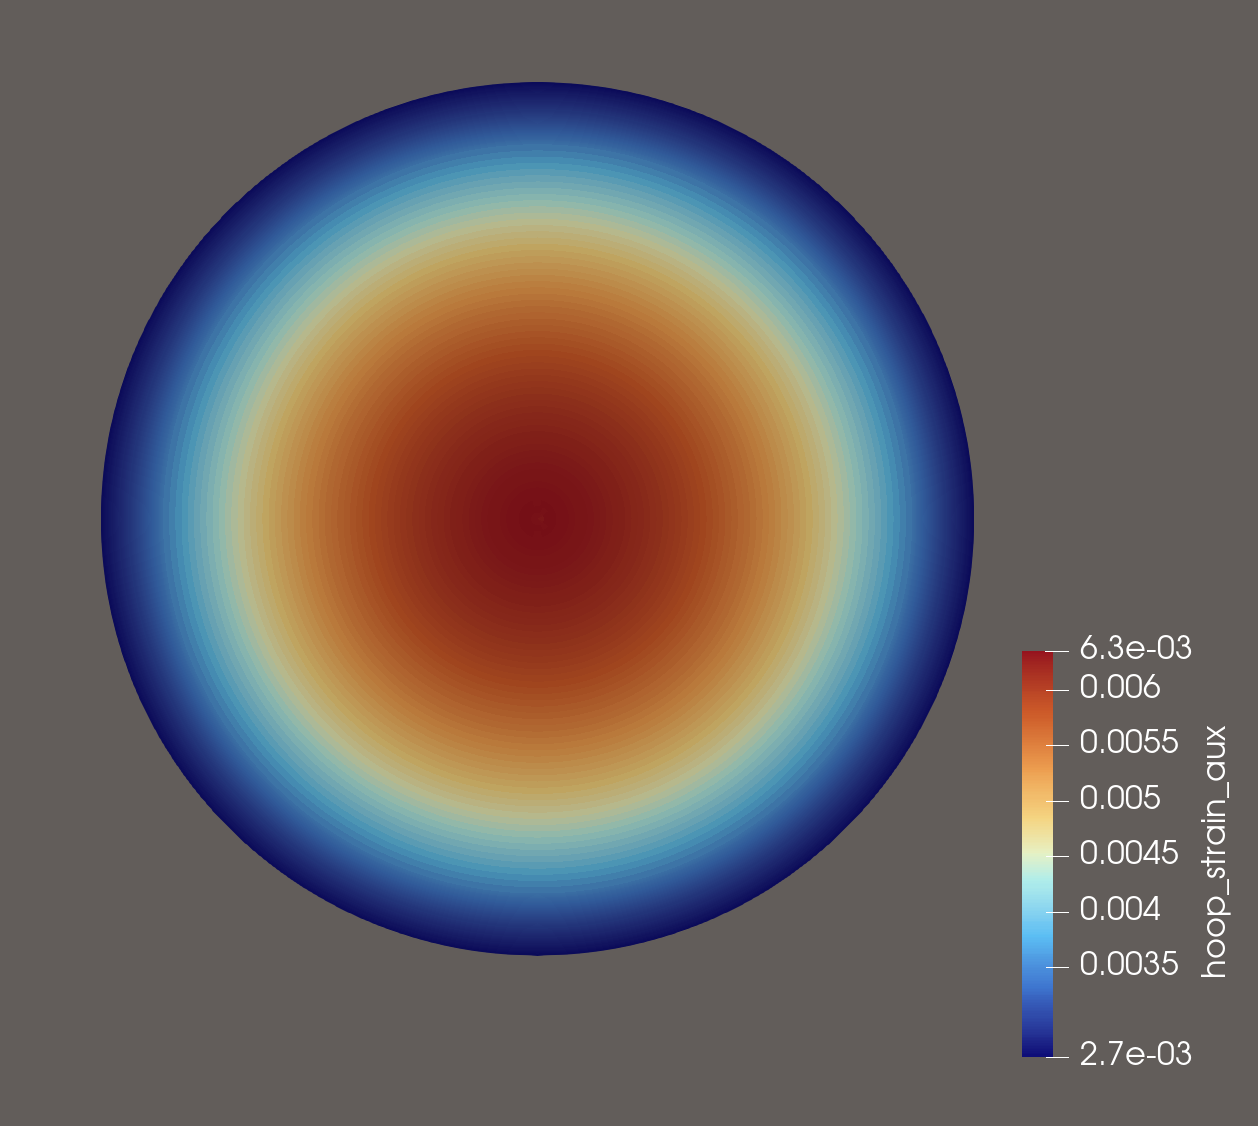
\includegraphics[width=0.5\linewidth]{figs/hoop_strain_TMI.png}
    \caption{Hoop strain profile at steady state during the operation of TMI-1.}
    \label{fig:placeholder}
\end{figure}

Displacement fields demonstrate outward radial expansion of the fuel, driven by thermal expansion. The magnitude of displacement is highest near the outer radius, indicating mechanical interaction with the cladding.

\begin{figure}[H]
    \centering
    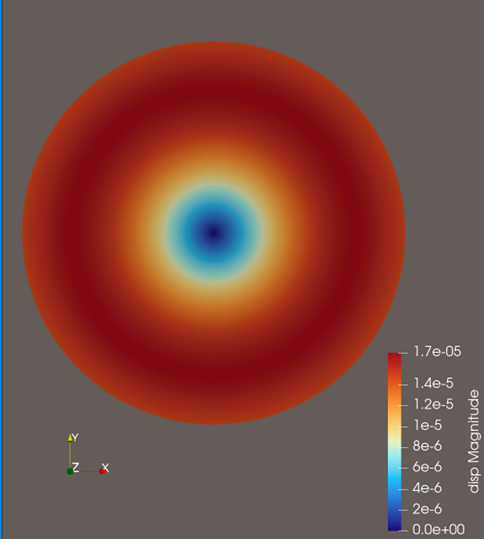
\includegraphics[width=0.5\linewidth]{figs/atomic-displacements-ss.png}
    \caption{Atomic displacements(m) of fuel and clad at steady state.}
    \label{fig:placeholder}
\end{figure}

In addition to the above variables, degradation factors specifically for the fuel and the clad were modeled as the fuel reached EOC. The conductivity and the stiffness were both degraded. These properties for the clad were also degraded simulating corrosion by the Arrhenius equation. Simultaneously, corrosion-driven degradation of the cladding further weakens its load-bearing capacity, setting the stage for failure under subsequent operating conditions.

\begin{figure}[H]
    \centering
    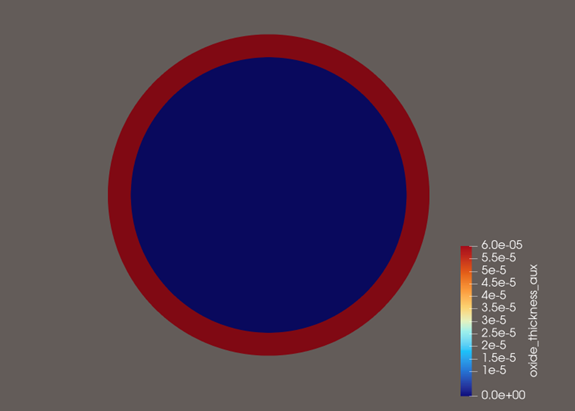
\includegraphics[width=0.5\linewidth]{figs/oxidation-eoc.png}
    \caption{The oxide growth thickness (m) due to corrosion at EOC.}
    \label{fig:placeholder}
\end{figure}

\subsection{Cooling Period}
The spent fuel was simulated as cooling in a wet storage pool for 20 years. In this model, no heat source was added, and corrosion of the cladding continued. The fuel is cooled down to 340 K after 20 years. During this period, volumetric contraction occurs, and some of the compressive stress built up during heating is released. However, due to irreversible nature of prior deformation, residual stresses remain within the cladding.

Despite the reduction in temperature, corrosion continues progressing due to a long exposure time. The oxide layer on the cladding surfaces grows to be nearly 0.45 mm over the storage period. This oxide buildup contributes to further conductivity degradation of the cladding and its mechanical stiffness, reducing its load-bearing capability and causing embrittlement.

These effects together result in a structurally weaker cladding before it is reheated in the LBR cycle. Although the mechanical state of the fuel element appears to be stable, it is in a drastically degraded condition with significantly reduced safety margins.
\begin{figure}[H]
    \centering
    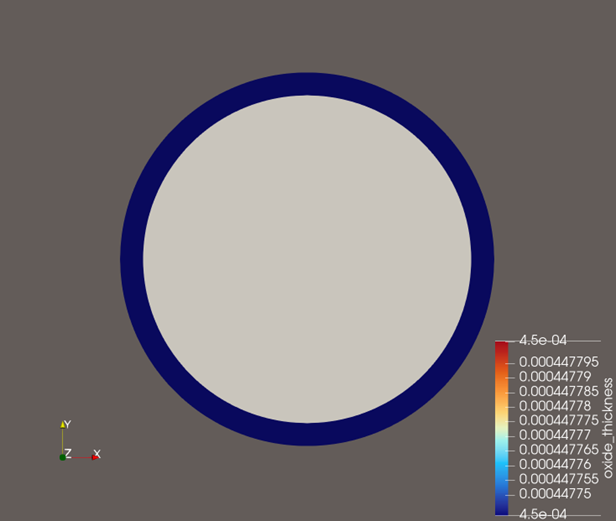
\includegraphics[width=0.5\linewidth]{figs/oxide-cool.png}
    \caption{Oxide buildup (m) on the clad surface.}
    \label{fig:placeholder}
\end{figure}

\begin{table}[H]
    \centering
    \caption{The properties for the clad before vs after heating and cooling}
    \label{tab:clad-props}
    \renewcommand{\arraystretch}{1.8}
    \begin{tabular}{>{\bfseries\raggedright\arraybackslash}m{3.8cm}
                    >{\centering\arraybackslash}m{2.5cm}
                    >{\centering\arraybackslash}m{2.8cm}}
    \toprule
    \makecell[l]{State} & \textbf{Conductivity (W/m-K)} & \textbf{Young's Modulus (Pa)}  \\
    \midrule
      Fresh & 17.0 & $1.0\times 10^{11}$ \\
      Degraded & 9.2 &  $6.9\times 10^{10}$  \\
    \bottomrule
    \end{tabular}
\end{table}

\subsection{Last Breath Reactor (Reheating Cycle)}

After the long heating and cooling periods, the spent fuel was subjected to the operating conditions of the Last Breath Reactor (LBR). The spent fuel was subjected to a volumetric heat of 305 MW/m$^3$ as derived from the thermalhydrauclics calculations, degraded conductivities of 2.5 and 9.2 W/(m-K) for the fuel and clad respectively, and a clad stiffness of 69 GPa, as obtained from the degradation mechanisms of prior simulations. Initially, for this part of the simulation, the Allen-Cahn phase field was turned on for the cladding to ensure it could survive the LBR cycle after extreme thermo-mechanical stresses. This is a genuine concern, as the LBR cycle uses a higher volumetric heat with poorer material properties, which hinders sufficient heat removal from the system, ramping up the thermal gradient and increasing the induced stresses even further.

 The thermal expansion, reduced stiffness, induced creep, and pre-existing corrosion damage cause the cladding to undergo severe thermomechanical loading. As observed by the fracture model, cracks propagate rapidly within a few days of operation. Normally, cracks are expected to propagate from the outer surface of the fuel, as shown in Figure 61 (b) for the TMI cycle, since ceramics tend to crack easily. However, cracking in Zircaloy-4, a metallic alloy, is an uncommon phenomenon that occurs directly. However, due to corrosion embrittlement and creep buildup, the cladding loses its structural integrity as a metal and begins to fracture or rupture.  

\begin{figure}[H]
    \centering
    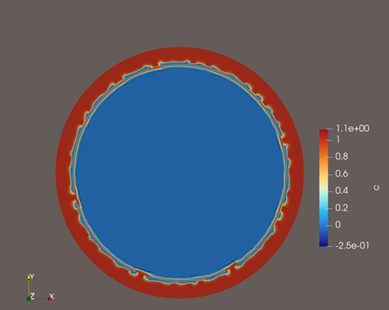
\includegraphics[width=0.49\linewidth]{figs/spent-fuel-cracks.png}
    \hfill
    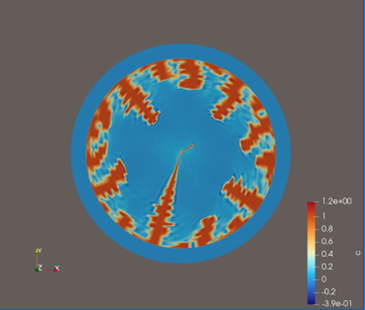
\includegraphics[width=0.49\linewidth]{figs/fresh-fuel-cracks.png}
    \caption{Crack propagation of (a) spent fuel (left) and (b) fresh fuel (right).}
    \label{fig:fuel-cracks}
\end{figure}

It should be noted that this model ignores irradiation induced damage and with the cladding already ruptured at the outer edges, there is  a significant risk, that the cracks would propagate enough, exposing the fuel region to the coolant. That would cause discharge of the fission products and gases into the coolant.

These results demonstrate that reuse of spent fuel without structural reinforcement is not viable under the aggressive thermal and mechanical environment of the LBR

\subsection{Failure Criteria and Safety Implications}

The structural integrity of the fuel–cladding system was evaluated using multiple failure criteria based on stress, creep deformation, and fracture mechanics.
Ductile failure in the cladding is assessed using the Von Mises yield criterion:
\begin{equation}
    \sigma_{vm}\geq\sigma_y
\end{equation}
where $\sigma_{vm}$ is the equivalent Von Mises stress and $\sigma_y$ is the yield strength of the material. When this condition is satisfied, plastic deformation and time-dependent creep mechanisms become dominant.
Creep rupture is further governed by the strong dependence of strain rate on stress and temperature, as previously described by the Norton–Arrhenius relation. Under elevated temperatures in the LBR cycle, even moderate stresses can lead to accelerated creep deformation, significantly reducing structural lifetime.

Meanwhile, a saturation-type corrosion model governs progressive oxide growth on the sleeve outer surface. This modulates both the elasticity and the conductivity of the sleeve. As corrosion progresses, the sleeve's conductivity degrades and raises local temperatures which accelerates creep. additionally, The degradation of conductivity and Young's modulus, substantially alters the stress redistribution at the fuel--clad interface.

Any single criterion by itself does not govern cladding failure. The simulation captures the synergistic interaction between thermally induced hoop stress, progressive creep strain accumulation in the clad, and the time-dependent stiffness reduction imposed by corrosion. Failure is considered to begin when the Von Mises stress  surpasses the  material yield strength in Zircaloy. A consequence of this is a structural lifetime limited by the rate of creep-driven strain under the degraded mechanical properties of the corroded Zircaloy. This coupled degradation route accelerates crack propagation in the cladding that highlights the need of a secondary containment system.


\subsection{Design of an Overclad}
\label{sec:overclad-design}
To prevent fuel failure through cladding rupture, the proposed solution for the last breath reactor would be to use an overclad coating. This coating layer would fit onto the clad like a sleeve. The material should be of good conductivity and high structural integrity.  The primary choice for this would be chromium, as Framatome has already been exploring chromium-coated fuel rods

\begin{figure}[H]
    \centering
    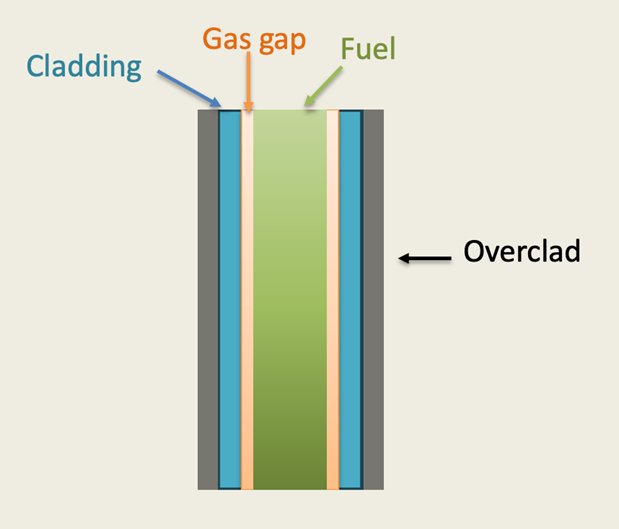
\includegraphics[width=0.5\linewidth]{figs/overclad-system.png}
    \caption{Overclad placement system.}
    \label{fig:placeholder}
\end{figure}

To choose a material for the overclad many things should be kept in mind. First and foremost, materialistic properties such as ability to withstand corrosion, the structural integrity, the penalty on neutronics, manufacturing feasibility and heat removal capabilities.

\textbf{Pure Chromium coating:}

Using a pure chromium coating, such as Framatome’s accident-tolerant fuel, would significantly improve corrosion resistance, as Chromium has an extremely low oxide pickup rate. It also has a very high thermal conductivity of 76 W/m-K at high temperatures, enabling exceptional heat transfer. However, the problem is that chromium cannot withstand the internal pressure if the cladding has already failed. The material is an exceptional coating choice for fresh fuel when the cladding has no pre-existing damage. Hence, there is a significantly high possibility that it would fail as a backup containment unit for the cladding \cite{BischoffCR-COATEDFRAMATOME}, \cite{Terrani2018AccidentChallenges}.%(Bischoff, J. et al., Framatome Chromium-Coated Zircaloy Cladding: From Development to Qualification, TopFuel 2018. The properties and ATF development context are also well documented in: Terrani, K.A., Accident Tolerant Fuel Cladding Development: Promise, Status, and Challenges, Journal of Nuclear Materials, Vol. 501, 2018. https://www.sciencedirect.com/science/article/pii/S002231151731342X)

\textbf{FeCrAl sleeve:}

The alloy of chromium mixed with iron and aluminum has quite an impressive ability to withstand internal pressure. In perfect-world conditions, this material would prove to be the ideal overclad material, as it can remove heat just as well as pure chromium. However, the biggest concern is that FeCrAl is a neutron absorber and can tax the reactor neutron  economy quite heavily thus impacting the power generation \cite{Lavrentiev2018Chromium-vacancyStudy}.

\textbf{SiC sleeve:}

The silicon carbide has a slightly poorer thermal conductivity, causing a poorer heat removal,  however it outperforms the prior choices in structural integrity, corrosion rates, and neutron economy. The biggest concern with this, however, is that it is currently quite difficult to manufacture, making it a much less feasible option \cite{Deck2015CharacterizationCladding}.

\textbf{Zircaloy-4} :

Probably one of the most conservative choices for the overcladding would be to use the cladding material itself to act as its backup containment. Having historically proven structural integrity, heat removal, and neutron economy, this material stands out the most to be the overcladding material, with the only concern being the impractical mechanisms of inserting the spent fuel into the zircaloy sleeve \cite{Motta2015CorrosionCladding}.%(Motta, A.T. et al., Corrosion of Zirconium Alloys Used for Nuclear Fuel Cladding, Annual Review of Materials Research, 2015. https://www.nuce.psu.edu/Motta/Publications/124_Motta_ARoMR_2015.pdf).


\begin{table}[H]
    \centering
    \caption{The decision-making model for overclad material selection.}
    \label{tab:decision_matrix-overclad}
    \renewcommand{\arraystretch}{1.8}
    \begin{tabular}{>{\bfseries\raggedright\arraybackslash}m{3.8cm}
                    >{\centering\arraybackslash}m{1.2cm}
                    >{\centering\arraybackslash}m{1.8cm}
                    >{\centering\arraybackslash}m{1.5cm}
                    >{\centering\arraybackslash}m{1.8cm}
                    >{\centering\arraybackslash}m{1.5cm}}
    \toprule
    \textbf{Criteria} & \textbf{Weight} & \textbf{Cr} & \textbf{FeCrAl} & \textbf{SiC} & \textbf{Zircaloy-4} \\
    \midrule
    Structural Strength        & 0.4 & 3 & 7 & 6 & 8 \\
    Neutron Economy            & 0.3 & 7 & 2 & 6 & 7 \\
    Heat Removal               & 0.2 & 9 & 8 & 5 & 6 \\
    Manufacturing Capability   & 0.1 & 6 & 6 & 2 & 4 \\
    \midrule
    \textbf{Total} & \textbf{1.0} & \textbf{5.70} & \textbf{5.6} & \textbf{5.4} & \textbf{6.9} \\
    \bottomrule
    \end{tabular}
\end{table}

The matrix weighs structural integrity as the highest (0.4) since cladding failure is the biggest concern of this simulation, as the overclad's sole function is to act as a secondary confinement layer. Neutron economy follows next (0.3), as excessive neutron absorption would penalize the reactor's already constrained fuel utilization. Heat removal was ranked next as the conductivity differences amongst the candidate materials are modest. Manufacturing capability was ranked last (0.1) despite being a real engineering problem, as it can be resolved with sufficient capital investment. Under this scheme, Zircaloy-4 scores the highest at 6.9 out of 10, primarily due to its structural strength and competitive performance across the other criteria, making it the most preferable candidate for the LBR concept.

\subsubsection{Materials testing for overclad}

In order to able to use fresh Zircaloy as the overclad, it must be ensured that it survives the conditions of the Last Breath Reactor cycle. It must be able to act as a secondary containment once the clad ruptures and holds back the fission products and the fuel particles from flowing into the coolant. Conservative guesses would assume that the overclad survives, since it is the same material as the original cladding, and since Zircaloy-4 is known to survive for an operating cycle of 5 years (which is also backed by previous simulations), it should be able to survive the smaller 300-day LBR cycle.

However, in this scenario, there is essentially no gas gap in between overclad and the cladding, and the ruptured cladding might exert additional pressure from the inside. Moreover, as the thermal simulations suggest higher temperatures for the cladding, the temperature coupled corrosion would be accelerated as well. Hence it was necessary to do the following simulations on MOOSE to make sure the overclad does not lose its structural integrity due to creep and corrosion.

\begin{figure}[H]
    \centering
    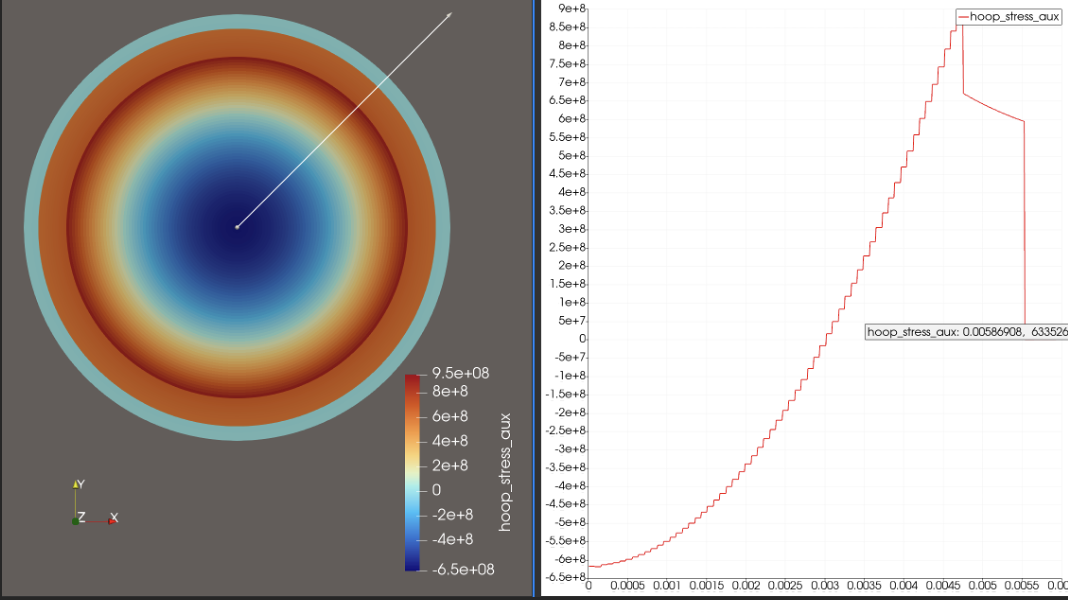
\includegraphics[width=0.8\linewidth]{figs/hoop_stress_LBR.png}
    \caption{Hoop stress (MPa) across the radial axis for the spent fuel with overclad at steady state in the Last Breath Reactor.}
    \label{fig:placeholder}
\end{figure}

\begin{table}[H]
    \centering
    \caption{The maximum hoop stress comparison between overclad and cladding in LBR vs TMI.}
    \label{tab:hoop-stress-comparison}
    \renewcommand{\arraystretch}{1.8}
    \begin{tabular}{>{\raggedright\arraybackslash}m{6cm}
                    >{\centering\arraybackslash}m{4cm}}
    \toprule
     & \textbf{Hoop Stress (MPa)} \\
    \midrule
    Fresh Zircaloy overclad in LBR & 0.633 \\
    Cladding in TMI                & 210   \\
    \bottomrule
    \end{tabular}
\end{table}

The hoop stress in the overclad is several orders of magnitude below that of the cladding in TMI. This can primarily be explained by the difference in inner pressure both elements experience. The overclad receives its inner pressure from the cladding, which is around 500~MPa for the LBR. Meanwhile in TMI, almost all the pressure the cladding receives is from the expansion of the fuel, which is around 900~MPa. In addition to PCI taking place, this significantly increases the pressure received by the cladding. The failed cladding also helps redistribute pressure from the outer clad surface onto the inner overclad surface.

\begin{figure}[H]
    \centering
    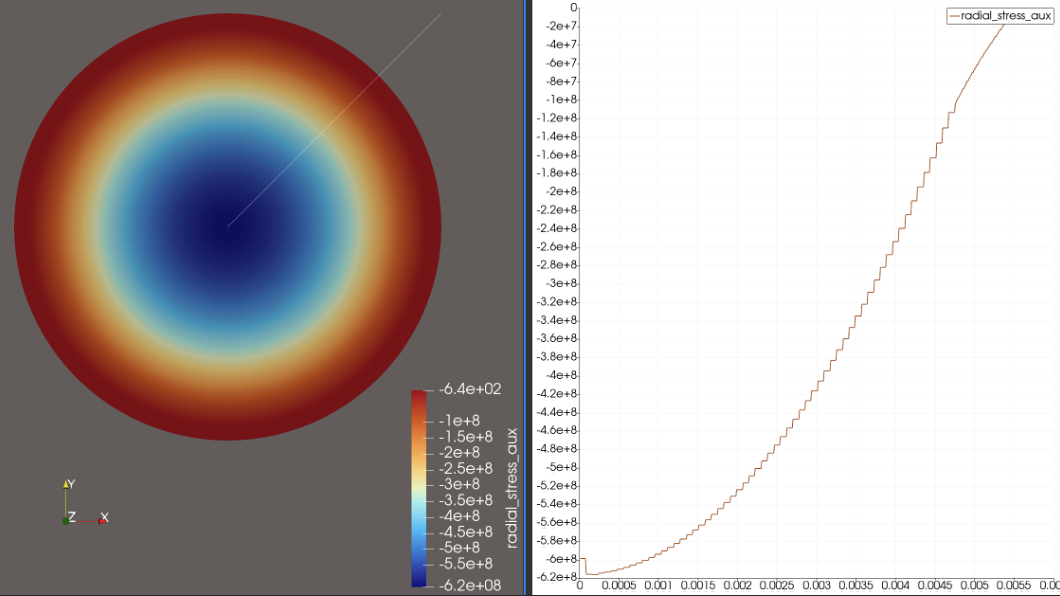
\includegraphics[width=0.8\linewidth]{figs/radial_stress_LBR.png}
    \caption{Radial stress (kPa) across the radial axis for the spent fuel with overclad at steady state in the Last Breath Reactor.}
    \label{fig:placeholder}
\end{figure}

\begin{table}[H]
    \centering
    \caption{The maximum radial stress comparison between overclad and cladding in LBR vs TMI.}
    \label{tab:radial-stress-comparison}
    \renewcommand{\arraystretch}{1.8}
    \begin{tabular}{>{\raggedright\arraybackslash}m{6cm}
                    >{\centering\arraybackslash}m{4cm}}
    \toprule
     & \textbf{Radial Stress (kPa)} \\
    \midrule
    Fresh Zircaloy overclad in LBR & 0.620 \\
    Cladding in TMI                & 210   \\
    \bottomrule
    \end{tabular}
\end{table}

Radial stress is equal to the contact pressure applied at the inner surfaces. The inner pressure from the cladding is lower in magnitude compared to the fuel inner pressure in the TMI cycle. This is further reduced due to the cracks and voids present in the ruptured cladding.

\begin{figure}[H]
    \centering
    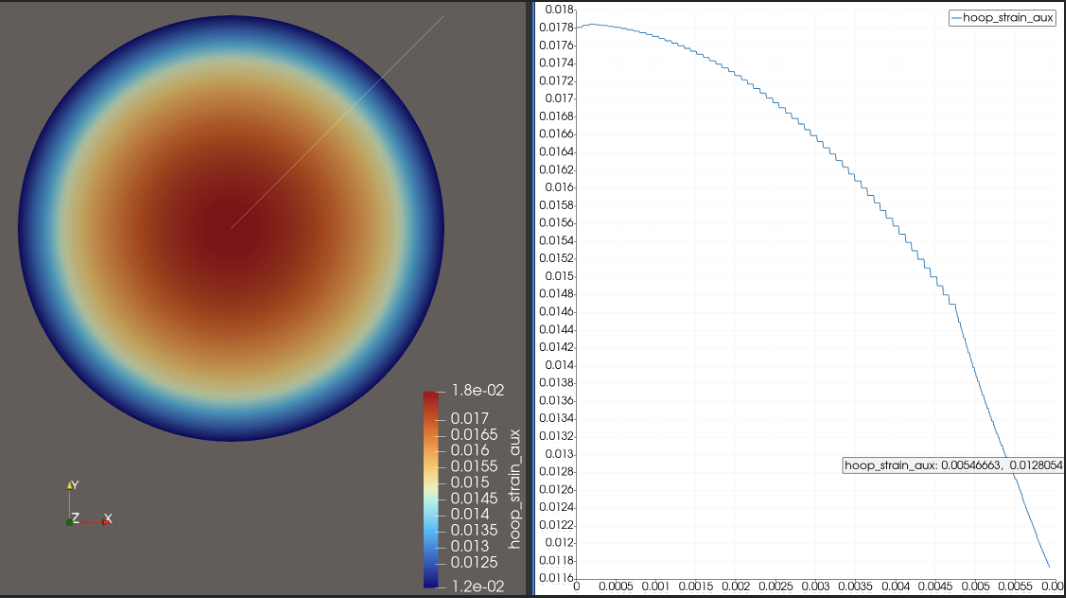
\includegraphics[width=0.8\linewidth]{figs/hoop_strain_LBR.png}
    \caption{Hoop strain across the radial axis for the spent fuel with overclad at steady state in the Last Breath Reactor.}
    \label{fig:placeholder}
\end{figure}

\begin{table}[H]
    \centering
    \caption{The maximum hoop strain comparison between overclad and cladding in LBR vs TMI at steady state.}
    \label{tab:hoop-strain-comparison}
    \renewcommand{\arraystretch}{1.8}
    \begin{tabular}{>{\raggedright\arraybackslash}m{6cm}
                    >{\centering\arraybackslash}m{4cm}}
    \toprule
     & \textbf{Hoop Strain} \\
    \midrule
    Fresh Zircaloy overclad in LBR & 0.013 \\
    Cladding in TMI                & 0.002 \\
    \bottomrule
    \end{tabular}
\end{table}

The hoop strain may appear concerning at first, as its magnitude in the overclad is higher than that of the cladding in TMI. However, the hoop strain is the sum of the creep strain, elastic strain, and thermal strain. The thermal strain, which drives thermal expansion, is considerably higher in the LBR cycle. The creep strain, governed by the Von Mises stress, is significantly lower in the overclad, as demonstrated by the following data.

\begin{figure}[H]
    \centering
    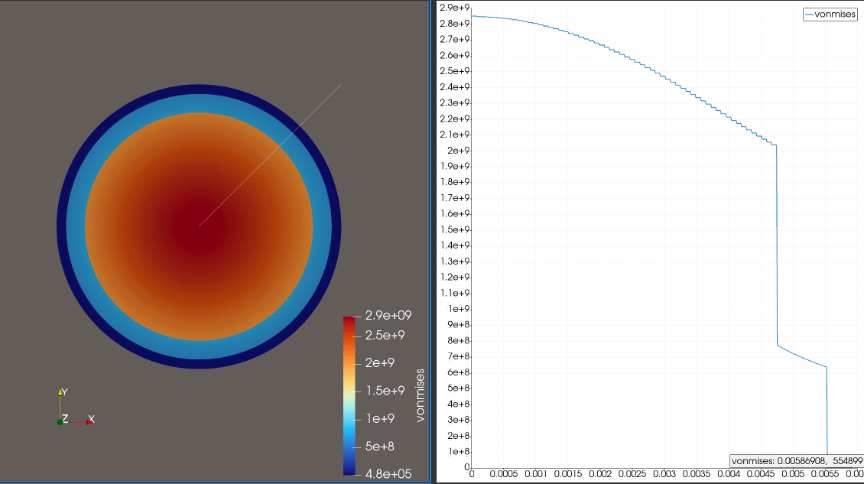
\includegraphics[width=0.8\linewidth]{figs/vonmises_LBR.png}
    \caption{Von Mises Stress (MPa) across the radial axis for the spent fuel with overclad at steady state in the Last Breath Reactor.}
    \label{fig:von-mises-overclad}
\end{figure}

\begin{table}[H]
    \centering
    \caption{Maximum Von Mises stress comparison between overclad and cladding in LBR vs TMI at steady state.}
    \label{tab:von-mises-comparison}
    \renewcommand{\arraystretch}{1.8}
    \begin{tabular}{>{\raggedright\arraybackslash}m{6cm}
                    >{\centering\arraybackslash}m{4cm}}
    \toprule
     & \textbf{Von Mises Stress (MPa)} \\
    \midrule
    Fresh Zircaloy overclad in LBR & 0.555 \\
    Cladding in TMI                & 160   \\
    \bottomrule
    \end{tabular}
\end{table}

The Von Mises stress is substantially lower for the overclad. Being the combined result of the hoop and radial stresses, the same reasoning regarding the ruptured cladding applies here. The lower Von Mises stress in the LBR overclad compared to the TMI cladding further ensures that the overclad will undergo significantly less creep and will maintain structural integrity over the 300-day operating cycle.

\begin{figure}[H]
    \centering
    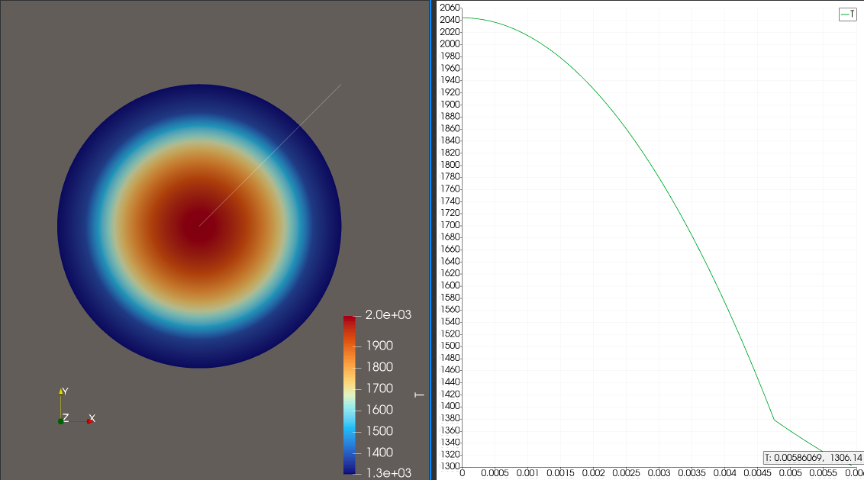
\includegraphics[width=0.8\linewidth]{figs/temp_LBR.png}
    \caption{Radial temperature profile (K) for the spent fuel with overclad at steady state in the Last Breath Reactor.}
    \label{fig:placeholder}
\end{figure}

\begin{table}[H]
    \centering
    \caption{Outermost edge temperature comparison between overclad and cladding in LBR vs TMI at steady state.}
    \label{tab:temp-comparison}
    \renewcommand{\arraystretch}{1.8}
    \begin{tabular}{>{\raggedright\arraybackslash}m{6cm}
                    >{\centering\arraybackslash}m{4cm}}
    \toprule
     & \textbf{Temperature (K)} \\
    \midrule
    Fresh Zircaloy overclad in LBR & 1306 \\
    Cladding in TMI                & 420  \\
    \bottomrule
    \end{tabular}
\end{table}

The overclad temperature is roughly three times higher than the clad temperature in TMI. This is due to a higher volumetric heat source being used with a poorer model of heat removal than that present in the TMI cycle. As corrosion is significantly sped up in higher temperatures, and operating in a long cycle would generally worsen the materials elasticity, the high temperature does raise a doubt in terms of overclad safety. However, these spent fuel rods will be under operation for 300 days in comparison to 5 years, so it would undergo less corrosion which is backed by the simulations data. On the other hand, the 1306K is under the NRC limit of 10 CFR 50.46, so no regulatory limits are being breached in this scenario \cite{NRC_50_46}. However, it must be noted that Zircaloy undergoes significant strength reduction at high temperatures. At room temperatures, the material has a yield strength of 500 MPa while reducing down to 100-150 MPa in the 1300 K temperature range \cite{NUREG/CR-6739Rods.}. Nevertheless, the Von Mises stress is only 0.555 MPa in the overclad, quite significantly below the yield strength ensuring the material is well within its elastic limit and is not in the risk of plastic collapse.%(Geelhood, K.J. and Luscher, W.G., FRAPTRAN-2.0: A Computer Code for the Transient Analysis of Oxide Fuel Rods, PNNL-19400, NRC, 2015. The material property models in this code document the temperature-dependent yield strength of Zircaloy-4. https://www.nrc.gov/docs/ML1611/ML16118A413.pdf)

\begin{figure}[H]
    \centering
    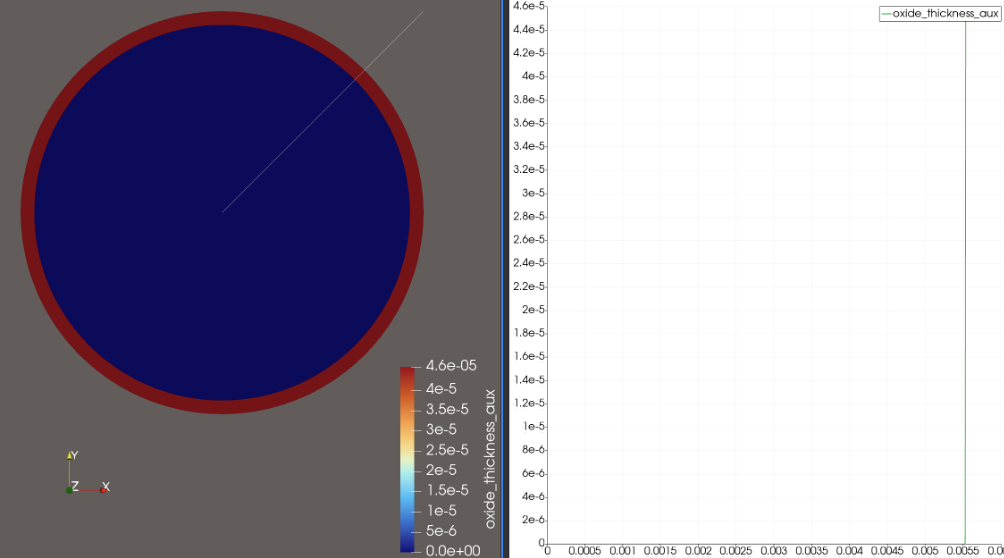
\includegraphics[width=0.8\linewidth]{figs/corrosion_LBR.png}
    \caption{Oxide growth (mm) across the radial axis for the spent fuel with overclad at steady state in the Last Breath Reactor.}
    \label{fig:placeholder}
\end{figure}

\begin{table}[H]
    \centering
    \caption{Oxide growth thickness comparison between overclad and cladding in LBR vs TMI at steady state.}
    \label{tab:oxide-growth-comparison}
    \renewcommand{\arraystretch}{1.8}
    \begin{tabular}{>{\raggedright\arraybackslash}m{6cm}
                    >{\centering\arraybackslash}m{4cm}}
    \toprule
     & \textbf{Oxide Growth (mm)} \\
    \midrule
    Fresh Zircaloy overclad in LBR & 0.046 \\
    Cladding in TMI                & 0.065 \\
    \bottomrule
    \end{tabular}
\end{table}

Although the elevated overclad temperature accelerates corrosion kinetics, the shorter 300-day LBR cycle results in less total oxide growth (0.046~mm) compared to the TMI cladding (0.065~mm). The risk of embrittlement-driven failure is therefore lower for the overclad, given that standard PWR cladding does not typically fail under the corrosion damage accumulated during a normal operating cycle.

\paragraph{Engineering Interpretation}

The introduction of a Zircaloy-4 overclad fundamentally alters the stress distribution within the fuel system by acting as a secondary structural barrier. In the absence of a gap, mechanical loads from the degraded cladding are directly transferred to the overclad, resulting in increased contact stresses. However, due to its intact mechanical properties, the overclad is capable of redistributing these stresses and preventing catastrophic failure.

Despite elevated temperatures and ongoing corrosion, the overclad maintains structural integrity throughout the LBR cycle, as indicated by the relatively low Von Mises stress compared to expected yield limits. This demonstrates that the overclad effectively compensates for the loss of strength in the original cladding.

These results suggest that the use of a Zircaloy-4 sleeve is a viable strategy for extending the operational lifetime of spent fuel under high-power conditions, provided that manufacturing and assembly challenges can be addressed.



\subsection{Model Validation and Physical Consistency}

To ensure the reliability of the simulation results, key outputs were compared against expected physical behavior and values reported in the literature.

The predicted centerline temperatures of $\sim$1100~K during the primary cycle are consistent with typical PWR fuel operating conditions, as reported in the nominal value of 1070~K in the Westinghouse PWR Systems Manual \cite{WestinghouseLimits}, %(NRC/Westinghouse Technology Systems Manual, Section 2.2, ML11223A208. https://www.nrc.gov/docs/ml1122/ML11223A208.pdf). 
 and are comparable to the 950--1150~K range validated by the FRAPCON-4.0 fuel performance code at similar power densities %(Geelhood, K.J. et al., FRAPCON-4.0: A Computer Code for the Calculation of Steady-State Thermal-Mechanical Behavior of Oxide Fuel Rods, PNNL-19418 Vol. 2 Rev. 2, NRC. https://www.nrc.gov/docs/ML1611/ML16118A434.pdf)
 \cite{2015FRAPCON-4.0Assessment.}. Likewise, the hoop stress distributions agree with the established PCMI behavior reported in the ORNL fuel cracking analysis \cite{Sweet2018AnalysisRelocation}, %(ORNL/TM-2018/889, Analysis of FeCrAl Cladding and UO₂ Fuel Including Discrete and Smeared Cracks. https://info.ornl.gov/sites/publications/Files/Pub112359.pdf
  and the maximum cladding hoop stress of 210~MPa lies within the 150--666~MPa range reported for PWR fuel rods \cite{Qi2020Pellet-claddingCladding}.%(Sercombe, J. et al., Pellet-cladding mechanical interaction analysis of Cr-coated Zircaloy cladding, Nuclear Engineering and Design, 2020. https://www.sciencedirect.com/science/article/pii/S0029549320302867).

The observed temperature increase during the LBR cycle is physically consistent with reduced thermal conductivity due to fuel degradation, combined with a higher volumetric heat source and reduced convective heat removal. The Arrhenius corrosion model aligns well with experimental data on PWR Zircaloy-4, where corrosion kinetics follow a cubic rate law with an activation energy of 132.8~kJ/mol \cite{osti_23002966}. %(Sato, T. et al., Autoclave Corrosion Experiment of Zircaloy-4 at Temperatures Between 180°C and 270°C, WM2019 Conference Proceedings, OSTI:23002966. https://www.osti.gov/biblio/23002966).
 Furthermore, the thermally driven corrosion behavior during the 20-year cooling period is consistent with established Zircaloy corrosion literature \cite{Motta2015CorrosionCladding}. %Motta, A.T. et al., Corrosion of Zirconium Alloys Used for Nuclear Fuel Cladding, Annual Review of Materials Research, 2015.: https://www.nuce.psu.edu/Motta/Publications/124_Motta_ARoMR_2015.pdf).

The predicted failure mode, characterized by cladding-initiated cracking driven by corrosion embrittlement, creep, and degraded material properties under high-temperature conditions, agrees with experimental observations on Zircaloy-4, where waterside corrosion produces a brittle hydride rim with significantly reduced fracture resistance under the multi-axial stress states induced during the LBR reheating cycle \cite{ONReader}. %(Daum, R.S. et al., On the Embrittlement of Zircaloy-4 under RIA-Relevant Conditions, ANL, 2001. https://publications.anl.gov/anlpubs/2001/12/41627.pdf)

Overall, the model captures the dominant physical mechanisms governing fuel--cladding behavior and provides results consistent with known reactor materials performance trends.

\subsection{Limitations and Future Work}

While the present model captures the key thermo-mechanical and degradation phenomena, several simplifying assumptions were made that may influence the accuracy of the results.

First, irradiation-induced effects such as swelling, fission gas release, and radiation hardening were not included. Neglecting fission gas pressure buildup in particular alters the hoop stress distribution. While these effects are secondary to thermo-mechanical stresses at the beginning of life, they become non-negligible at the end of the cycle. FRAPCON simulations of comparable PWR fuel rods indicate that internal fission gas pressure at the end of the cycle can contribute an additional 50--100~MPa of hoop stress to the cladding \cite{2015FRAPCON-4.0Assessment.}, %(Geelhood, K.J. et al., FRAPCON-4.0: A Computer Code for the Calculation of Steady-State Thermal-Mechanical Behavior of Oxide Fuel Rods, PNNL-19418 Vol. 2 Rev. 2, NRC. https://www.nrc.gov/docs/ML1611/ML16118A434.pdf).
 meaning the LBR cladding and overclad stresses are likely underestimated.

Additionally, the corrosion model is simplified and does not account for complex oxide layer behavior, such as spallation or transition kinetics. The exclusion of these phenomena results in an underestimate of the peak corrosion rates of Zircaloy in reactor conditions as corrosion rates are known to accelerate to a factor of 6 when fuel undergoes multiple irradiation cycles %(Blat, M. and Noel, D., Analysis of the Waterside Corrosion Kinetics of Zircaloy-4 Fuel Cladding in French PWRs, Nuclear Technology, Vol. 170, 2010.  https://www.tandfonline.com/doi/abs/10.13182/NT10-A10330)
\cite{Bouineau01062010}. The phase-field fracture model, while effective in capturing crack propagation, does not explicitly resolve microstructural mechanisms such as grain boundary failure.

Ignoring the fuel gas gap in the primary cycle simulates the fuel having more heat removal than normal, resulting in a much cooler fuel as it is the strongest element of thermal resistance. This means that the model assumes direct conductive contact across the fuel–cladding interface, artificially enhancing heat removal from the fuel and resulting in a non-conservative underestimate of the fuel centerline temperature %(Lapetite, J.M. et al., Measurement of the Thermal Conductivity of Metal Clad Uranium Oxide Rods During Irradiation, Journal of Nuclear Materials, 1961. https://www.sciencedirect.com/science/article/abs/pii/0022311561902021)
\cite{Cohen1961MeasurementIrradiation}. However, it should be addressed that the gas gap limitation applies to the primary heating cycle and during the LBR heating phase, the ruptured cladding is in direct contact with the overclad, which makes the no gas-gap assumption an approximation that is much closer to reality for that stage of the simulation.

Future work should include irradiation effects with detailed neutron fluence data, burnup tracking and DPA (displacement per atom) evolutions, which would allow to simulate DPA correlations, swelling laws and irradiation creep coefficients that can be cross-checked with more advanced models such as BISON or FRAPCON. With the availability of sufficient computational power, these simulations can be rerun with the more advanced corrosion kinetics, a detailed phase field fracture physics and including gap mechanics.

\clearpage

% ===================================================================
% ECONOMICS
% ===================================================================
\section{Economic and Infrastructure Analysis (D. Frank)}
The closest parallel to the Last Breath Reactor concept is the \textit{Direct Use of PWR Fuel In CANDU Reactors} (DUPIC) fuel cycle, first proposed in 1997 by J.~Lee et al.~\cite{LeeTHEHWR}. Both LBR and DUPIC require dedicated facilities capable of receiving and processing spent PWR assemblies at scale under full hot-cell shielding. The principal distinction is that LBR bypasses the chemically and thermally intensive OREOX--pelletisation--sintering overall capital and operating costs are consequently projected to be substantially lower.

%------------------------------------------------------------------
\subsection{Process Step Comparison}
%------------------------------------------------------------------

\noindent\textbf{DUPIC.}\;
Spent PWR assemblies are disassembled and mechanically decladded to
produce loose pellet fragments, which are subjected to repeated
\textit{OREOX} cycling
(UO$_2\!\to$U$_3$O$_8$ at 400 \textdegree C,
U$_3$O$_8\!\to$UO$_2$ at 600 \textdegree C, three cycles),
milled, cold-pressed, sintered at 1,650--1,850\textdegree C, ground, and loaded into fresh Zircaloy-4 rods to form
43-element CANFLEX bundles for use in CANDU heavy-water reactors.

\medskip
\noindent\textbf{LBR.}\;
Spent PWR assemblies are accepted as-is---the original cladding is never breached. Each fuel rod is slid into a close-fitting Zircaloy-4 overclad sleeve (described in \S\ref{sec:overclad-design}), whose end-caps are remote-welded and helium-backfilled, leak-tested, and NDA-assayed. 192 overcladded rods are then integrated into a 15$\times$15 structural skeleton at a 6-cm lattice pitch for use in a heavy-water-moderated reactor.

\medskip
\renewcommand{\arraystretch}{1.20}
\begin{tabularx}{\linewidth}{L{4.8cm} C{1.55cm} C{1.55cm} L{5.6cm}}
\toprule
\textbf{Step} & \textbf{DUPIC} & \textbf{LBR} & \textbf{Note} \\
\midrule
Receiving \& characterisation    & \checkmark & \checkmark
  & Identical requirements \\
Disassembly (rod extraction)     & \checkmark & \checkmark
  & Both require hot-cell remote ops \\
Decladding                       & \checkmark & ---
  & \textbf{Eliminated in LBR} \\
OREOX cycling                    & \checkmark & ---
  & \textbf{Eliminated in LBR} \\
Powder milling, blending, pressing & \checkmark & ---
  & \textbf{Eliminated in LBR} \\
Sintering (1,650--1,850 \textdegree C) & \checkmark & ---
  & \textbf{Eliminated in LBR} \\
Pellet centreless grinding       & \checkmark & ---
  & \textbf{Eliminated in LBR} \\
New Zircaloy-4 pin loading       & \checkmark & ---
  & Replaced by overclad step \\
Overclad sleeve installation     & ---        & \checkmark
  & \textbf{Added in LBR} \\
Assembly integration             & \checkmark & \checkmark
  & CANFLEX 43-element vs.\ 15$\times$15 \\
\bottomrule
\end{tabularx}

%------------------------------------------------------------------
\subsection{Cost Methodology}
%------------------------------------------------------------------

LBR fabrication costs are estimated by applying scaling factors to the detailed, compartmentalised economic analysis of DUPIC published by Ko, Choi, and Yang in 2001~\cite{Ko2001EconomicCost}. All figures in that study are reported in December~1999 USD; a U.S.\ CPI escalation factor of 1.96 is applied throughout to convert to March~2026 USD. The original study amortises capital expenditures over a 40-year plant life at a 5\% discount rate with a 25\% contingency allowance. Six scaling rules are applied to derive LBR costs:

\begin{enumerate}
    \item \textbf{Capital at 35\% of DUPIC.}
          OREOX oven banks, sintering furnaces, and powder-handling
          cells represent $\approx$65\% of the \$326.6M
          process-systems direct capital; these are entirely absent
          in LBR.

    \item \textbf{Labour at 50\% of DUPIC.}
          LBR requires $\approx$250 staff versus $\approx$500 for
          DUPIC; OREOX, powder, and sintering operators are
          not needed.

    \item \textbf{Utilities at 33\% of DUPIC.}
          A conservative estimate of the savings achieved by
          eliminating the OREOX and high-temperature sintering loads.

    \item \textbf{Process radwaste at 9\% of DUPIC.}
          The Zircaloy cladding-hull stream
          (0.29 t/tHM,$\approx$116 t/yr at reference throughput)
          is entirely eliminated; only the structural hardware waste
          stream (0.07 t/tHM) remains.

    \item \textbf{Back-end costs retained at the DUPIC rate.}
          Spent LBR assemblies carry a comparable fission-product
          inventory and decay-heat profile to spent CANDU-DUPIC fuel;
          interim storage and geological disposal requirements are
          essentially unchanged.

    \item \textbf{Materials at 150\% of DUPIC.}
          A conservative premium to account for the fuelled
          power-inverter rods (PI-F) specific to LBR.
          Both systems require fresh cladding and structural
          assembly components; DUPIC additionally requires dysprosium
          poison rods.
\end{enumerate}

%------------------------------------------------------------------
\subsection{Compartmentalised Cost Breakdown}
%------------------------------------------------------------------

\renewcommand{\arraystretch}{1.22}
\begin{tabularx}{\linewidth}{L{7.5cm} R{2.2cm} R{2.2cm} R{1.6cm}}
\toprule
\textbf{Cost element}
  & \textbf{DUPIC} & \textbf{LBR}
  & \textbf{LBR \%} \\
  & \textbf{(\$/kgHM)} & \textbf{(\$/kgHM)} & \\
\midrule
Capital --- site preparation, process systems,
  hot-cell building, indirect costs
  & 563 & 197 & 35\% \\
Labour --- 500 vs.\ 250 staff
  & 118 & 59  & 50\% \\
Utilities --- electricity, steam, chemicals
  & 49  & 16  & 33\% \\
Materials --- cladding, structural skeleton, PI-F rods
  & 98  & 196 & 200\% \\
Process radwaste --- cladding hulls, off-gas,
  structural, miscellaneous LLW
  & 367 & 33  & 9\%  \\
\midrule
\textbf{Fabrication total}
  & \textbf{1,195} & \textbf{501} & \textbf{42\%} \\
\midrule
Back-end --- transport, fuel handling, interim
  storage, geological disposal
  & 1,158 & 1,158 & 100\% \\
\midrule
\textbf{Grand total}
  & \textbf{2,353} & \textbf{1,659} & \textbf{71\%} \\
\bottomrule
\end{tabularx}

%------------------------------------------------------------------
\subsection{Specific Cost Comparison}
%------------------------------------------------------------------

Table~\ref{tab:specific-cost} compares the three fuel concepts on a specific-cost basis. The average LBR power density of 13.45 kW/kgHM follows from the 30 kW/kgHM peak limit (\S\ref{sec:temp-limits}) and the power-peaking factor of 2.23 (\S\ref{sec:pi-f-final}). CANDU reactors (used for DUPIC) operate at $\approx$25 kW/kgHM, and the conventional PWR reference case uses 40 kW/kgHM as specified by the user.

For the cost per unit of energy (\$/MWd), only the incremental burnup extracted in the heavy-water reactor is attributed to the refabrication cost, since the feedstock fuel has already produced approximately 45 MWd/kgHM during its original PWR irradiation. DUPIC extends total accumulated burnup to 58 MWd/kgHM~\cite{Mohamed2016EffectParameters}, yielding 13 MWd/kgHM additional; LBR reaches 60 MWd/kgHM (\S\ref{sec:pi-f-final}), yielding 15 MWd/kgHM additional. The conventional PWR figure uses the full 45 MWd/kgHM discharge burnup against the complete front- and back-end fuel cycle cost of \$2,982/kgHM~\cite{TheCosts}.

\begin{table}[H]
\centering
\caption{Specific fuel cost comparison across the three reactor
  concepts (March~2026 USD).
  For DUPIC and LBR the \$/MWd figure uses only the incremental
  burnup achieved in the heavy-water reactor; for the conventional
  PWR it uses the full discharge burnup.}
\label{tab:specific-cost}
\renewcommand{\arraystretch}{1.35}
\begin{tabularx}{\linewidth}{L{4.6cm}
                              R{2.2cm} R{2.2cm} R{2.2cm}}
\toprule
\textbf{Metric}
  & \textbf{Conv.\ PWR}
  & \textbf{DUPIC}
  & \textbf{LBR} \\
\midrule
Total fuel cost (\$/kgHM)
  & 2,982 & 2,353 & 1,659 \\
Specific power (kW/kgHM)
  & 40     & 25     & 13.45  \\
Incremental burnup (MWd/kgHM)
  & 45     & 13     & 15     \\
\midrule
\textbf{Cost per unit power (\$/kW)}
  & \textbf{74.6} & \textbf{94.1} & \textbf{123.3} \\
\textbf{Cost per unit energy (\$/MWd)}
  & \textbf{66.3} & \textbf{181.0} & \textbf{110.6} \\
\bottomrule
\end{tabularx}
\end{table}

\noindent
The conventional PWR achieves the lowest cost on both metrics because it burns a large fraction of its fissile loading at high specific power with no refabrication overhead. LBR outperforms DUPIC on \$/MWd (110.6 vs.\ 181.0) because it extracts slightly more incremental energy (15 vs.\ 13 MWd/kgHM) at substantially lower fabrication cost; however, its lower operating power density (13.45 vs.\ 25 kW/kgHM) results in a higher \$/kW figure. The \$/MWd figures for DUPIC and LBR do not include the cost of the original PWR fuel cycle; the relevant economic comparison is against the \emph{avoided} direct-disposal cost of $\approx$\$1,195/kgHM, which represents the back-end cost the utility would otherwise incur for the spent PWR assemblies. On that basis the net marginal cost of extracting additional energy from spent fuel is \$1,158/13 $=$ \$89/MWd for DUPIC and \$464/15$=$\$31/MWd for LBR, both substantially below the conventional PWR reference of \$66/MWd.

\clearpage

% ===================================================================
% DESIGN CONCEPT SUMMARY
% ===================================================================
\section{Design Concept Summary (All)}
% ============================================================
%  DESIGN CONCEPT SUMMARY
% ============================================================

The LBR is a heavy-water-moderated, heavy-water-cooled reactor operating at
10\,MPa with a thermal output of 2.0\,GW$_\text{th}$. Spent PWR fuel
assemblies are accepted without mechanical or chemical processing; each
individual fuel rod is enclosed in a close-fitting Zircaloy-4 overclad sleeve
whose end-caps are remote-welded, helium-backfilled, and leak-tested before
integration into the core structure. The design philosophy is one of minimum
intervention: every refabrication step that can be eliminated is eliminated.

% ============================================================
\subsection{Core Layout and Operating Parameters}
% ============================================================

The active core is composed of assemblies arranged on a 6\,cm square lattice
pitch. Each assembly is built around a 15$\times$15 structural skeleton;
of the 225 available lattice positions, 192 are occupied by overcladded spent
fuel rods and 25 are occupied by Fueled Power Inverter (PI-F) devices
distributed at alternating positions throughout the assembly. At a specific
power of 30\,W/gHM, the 2\,GW$_\text{th}$ thermal output requires
approximately 67\,tonnes of heavy metal distributed across $\sim$19\,400 fuel
rods. Primary operating parameters are summarized in
Table~\ref{tab:core_params}.

\begin{table}[H]
\centering
\caption{Summary of primary LBR core design parameters.}
\label{tab:core_params}
\renewcommand{\arraystretch}{1.35}
\begin{tabular}{l l}
\toprule
\textbf{Parameter} & \textbf{Value} \\
\midrule
Thermal output              & 2.0\,GW$_\text{th}$ \\
Moderator / coolant         & Heavy water (D$_2$O) \\
Operating pressure          & 10\,MPa \\
Coolant inlet / outlet      & 533\,K / 582\,K \\
Specific power              & 30\,W/gHM \\
Lattice pitch               & 6\,cm (square) \\
Assembly layout             & 15$\times$15 \\
Spent fuel positions / assembly & 192 \\
PI-F positions / assembly   & 25 \\
Total heavy metal inventory & $\approx$67\,t \\
Total fuel rods (core)      & $\approx$19\,400 \\
Design discharge burnup     & 60.1\,GWd/tHM \\
Power peaking factor (PPF)  & 2.23 \\
DNBR (hot channel)          & 2.95 \\
\bottomrule
\end{tabular}
\end{table}

The spent fuel feedstock is characterized by an initial enrichment of
$\sim$4.01--4.5\,wt.\% $^{235}$U and a discharge burnup of
$\sim$47--53\,GWd/tHM from PWR service, representative of assemblies from
the U.S. commercial fleet. Fuel compositions were generated by a
Serpent~2 depletion model benchmarked against the TMI-1 NJ05YU assembly
post-irradiation examination data and transferred to the LBR lattice model
via binary restart file, preserving the full axially resolved nuclide
inventory.

% ============================================================
\subsection{Overclad Sleeve and Fuel Rod Preparation}
% ============================================================

The overclad is a close-fitting Zircaloy-4 tube into which a spent PWR fuel
rod is inserted without breaching the original cladding. End-caps are
remote-welded under hot-cell conditions, after which the annular space is
helium-backfilled to a specified pressure, leak-tested, and subjected to
non-destructive assay to confirm fuel rod identity. The overclad outer
diameter and wall thickness are chosen to maintain the same rod outer
dimension as the PI-F rods, so that all lattice positions share a uniform
pitch geometry. This design preserves the original spent fuel cladding as a
first barrier, adds the overclad as a second barrier, and avoids all
high-activity powder handling operations. The result is a dramatically
simplified hot-cell processing chain relative to DUPIC, as quantified in
Section~\ref{sec:economics}.

% ============================================================
\subsection{Fueled Power Inverter Device}
% ============================================================

The Fueled Power Inverter is the primary novel component of the LBR assembly.
It is a fresh UO$_2$ fuel rod with a graded axial enrichment profile designed
to concentrate fission power in the axially under-depleted extremities of
adjacent spent rods---the regions where PWR irradiation history leaves the
highest residual fissile inventory.

The device geometry matches the outer dimensions of the overcladded spent fuel
rods: Zircaloy-4 cladding with a 10.92\,mm outer diameter and an active fuel
length of 360.17\,cm. The axial enrichment profile consists of two zones:
\begin{itemize}
    \item \textbf{End regions} (upper and lower $\sim$70\,cm): 4.5\,wt.\%
    $^{235}$U --- co-located with the under-depleted extremities of the
    surrounding spent rods, where the additional reactivity drives enhanced
    local fission rates and ``inverts'' the axial power peak toward the rod
    ends.
    \item \textbf{Central region} ($\sim$220\,cm): 3.5\,wt.\% $^{235}$U ---
    co-located with the high-burnup midplane of adjacent spent rods, where
    lower enrichment limits the power contribution from the fresh fuel
    without suppressing criticality.
\end{itemize}

This configuration was selected from a parametric enrichment sweep (central
enrichments 1.25--8.25\,wt.\%, edge enrichments always $>$ central) on the
basis of a weighted decision matrix prioritizing critical cycle length
(weight 0.40) and power peaking factor (weight 0.35). The 3.5\,/\,4.5\,wt.\%
combination uniquely satisfies both the 60\,GWd/t burnup objective and the
PPF\,$\leq 2.5$ safety objective. The resulting bimodal axial power
distribution---fission peaks at the rod ends flanking a lower-power
midplane---is the defining neutronics signature of the LBR design. A detailed
description of Power Inverter geometry, materials, and fabrication
considerations is provided in Appendix~\ref{sec:app_A}.

% ============================================================
\subsection{Relationship to CANDU and the DUPIC Fuel Cycle}
% ============================================================

The LBR shares architectural heritage with the CANDU reactor family. Both
systems exploit D$_2$O moderation to maintain criticality on sub-enriched
fuel, and both can in principle be operated with online or near-online
refueling that eliminates the large initial excess reactivity burden of batch
refueling. The closest antecedent to the LBR concept is the DUPIC (Direct Use
of PWR Fuel In CANDU) cycle, which also proposes loading spent PWR fuel into
a heavy-water reactor without chemical separation. Table~\ref{tab:dupic_lbr}
summarizes the key distinctions.

\begin{table}[H]
\centering
\caption{Comparison of DUPIC and LBR fuel cycle process steps and key
metrics (March~2026 USD).}
\label{tab:dupic_lbr}
\renewcommand{\arraystretch}{1.30}
\begin{tabular}{l c c}
\toprule
\textbf{Attribute} & \textbf{DUPIC} & \textbf{LBR} \\
\midrule
Decladding required             & Yes               & No \\
OREOX cycling                   & Yes               & No \\
High-temperature sintering      & Yes (1650--1850\,$^\circ$C) & No \\
Pellet grinding                 & Yes               & No \\
New cladding required           & Yes (CANFLEX)     & Overclad sleeve only \\
Assembly geometry               & 43-element CANFLEX & 15$\times$15, 6\,cm pitch \\
Cladding-hull waste stream      & Yes               & \textbf{Eliminated} \\
Fabrication cost (\$/kgHM)      & 1,195             & 501 \\
All-in lifecycle cost (\$/kgHM) & 2,353             & 1,659 \\
Incremental burnup (MWd/kgHM)   & 13                & 15 \\
Incremental energy cost (\$/MWd)& 181               & 111 \\
\bottomrule
\end{tabular}
\end{table}

The key differentiator is the elimination of the thermo-chemical refabrication
chain. Because the original cladding is never breached, LBR does not generate
the Zircaloy cladding-hull waste stream (0.29\,t/tHM in DUPIC) that
constitutes the dominant component of DUPIC's process radwaste cost, and it
avoids the OREOX cycling, powder handling, and sintering operations that
account for $\sim$65\% of DUPIC's direct capital cost. The tradeoff is
reduced geometric flexibility: the LBR must accommodate the existing PWR rod
dimensions and axial composition profile, which drove the development of the
Power Inverter concept as a power-shaping tool.

% ============================================================
\subsection{Materials Summary}
% ============================================================

The primary materials employed in the final LBR design are:

\begin{itemize}
    \item \textbf{Fuel}: Commercial UO$_2$ as discharged from PWR service,
    with initial enrichment $\approx$4.01--4.5\,wt.\% and discharge burnup
    $\approx$47--53\,GWd/t. The PI-F rods use fresh UO$_2$ at graded
    enrichments of 3.5\,wt.\% (center) and 4.5\,wt.\% (edge).

    \item \textbf{Cladding and overclad}: Zircaloy-4, selected for its
    established neutron irradiation performance database, compatibility with
    pressurized D$_2$O coolant at 10\,MPa and 533--582\,K, and low thermal
    neutron absorption cross section. Thermal conductivity is conservatively
    taken as 9.2\,W/m-K (degraded spent-fuel value) for thermal analysis.

    \item \textbf{Moderator and coolant}: Heavy water (D$_2$O) at 10\,MPa.
    Properties used in thermal-hydraulic analysis: $\rho = 874$\,kg/m$^3$,
    $c_p = 4670$\,J/kg-K, $k = 0.53$\,W/m-K, $\mu = 1.14\times10^{-4}$\,kg/m-s.

    \item \textbf{Structural components}: Stainless steel (SS-304) for
    assembly grid spacers, end fittings, upper and lower plenums, and pressure
    boundary hardware, consistent with the TMI-1 reference assembly geometry.
\end{itemize}

The structural integrity and lifetime performance of the fuel-cladding system
under irradiation, thermal cycling, and corrosion were evaluated in
Section~\ref{sec:Materials} using the MOOSE multiphysics finite element
framework, coupling heat conduction, solid mechanics, creep deformation, and
corrosion-induced property degradation.



\clearpage

% ===================================================================
% CONCLUSIONS
% ===================================================================
\section{Conclusions and Recommendations (All)}
\textbf{Neutronics}

From a neutronics perspective, Last Breath Reactor has proven the capability of generating thermal energy from spent nuclear fuel rods while simultaneously reducing the quality of plutonium. With the use of the \textit{Power Inverter}, LBR can sustain criticality up to an averaged burnup of 61.6 GWd. However, the Power Inverter introduces a proliferation risk -- containg weapons grade plutonium at the end of cycle -- and diverts from the central goal of avoiding fresh fuel usage. A better approach might be optimizing a fuel reloading pattern such that burnup can be even further extended without relying on fresh fuel. This is a complex optimization problem that must consider fission project generation, structural integrity, and neutron economy.


\textbf{Structural \& Operational}
The 6-cm lattice pitch will make the reactor considerably large. To mitigate the sheer size, the reactor should operate with a power density that is large, but reasonable enough to meet materials and thermal-hydraulics safety margins. With a higher power density comes faster depletion -- to make operation economical, the reactor vessel should be designed for on-line reloading. Some considerations should be made about vessel orientation, the use of pressure tubes (like a CANDU), etc.



\clearpage
\newpage



% ===================================================================
% REFERENCES
% ===================================================================
\printbibliography


\clearpage

% ===================================================================
% APPENDICES
% ===================================================================
\appendix

\section{Power Inverter Details (D. Frank)}
\label{sec:app_A}
\begin{figure}[h]
    \centering
    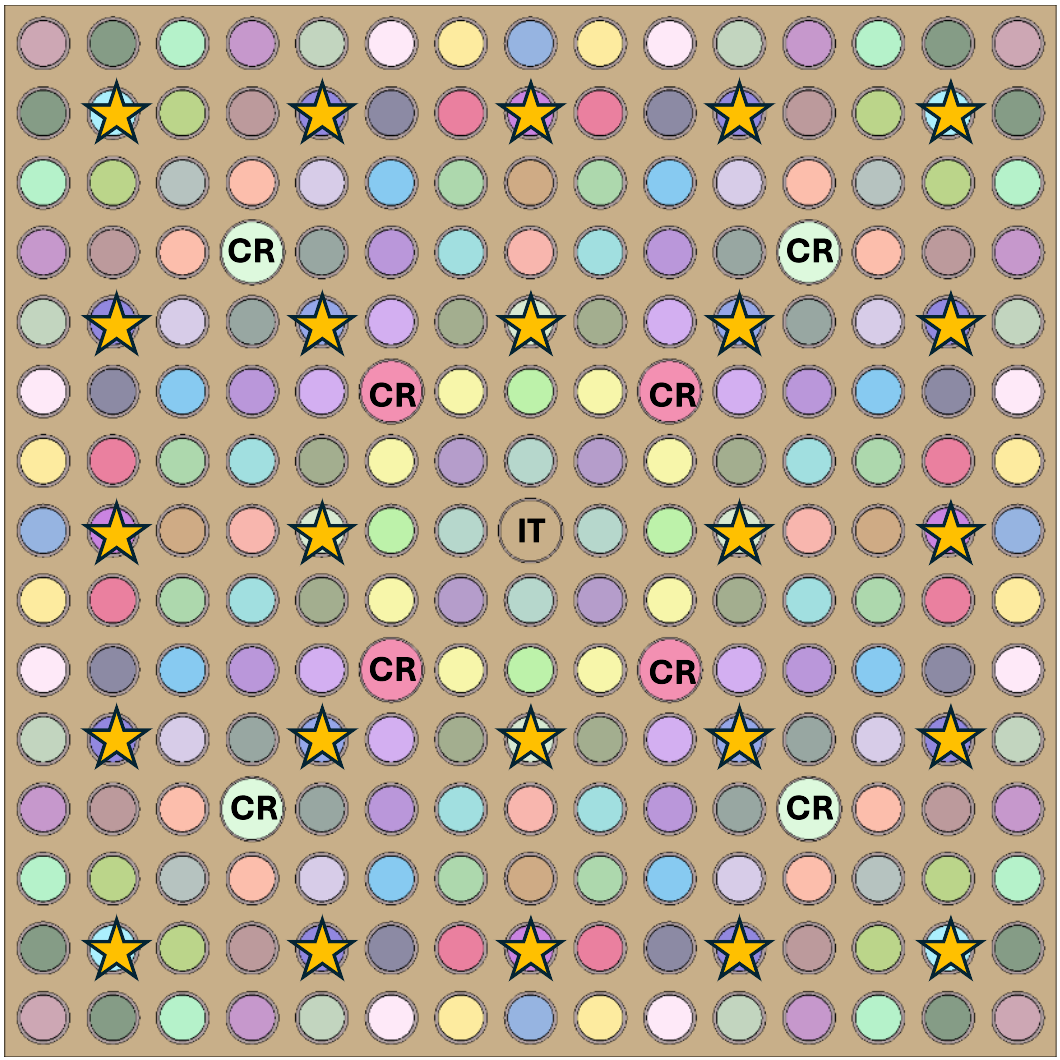
\includegraphics[width=0.5\linewidth]{appendices/CoreLayout.png}
    \caption{Cross section of the assembly layout. The stars show the positions of the power inverter devices, rods labeled \textit{CR} are control rods, and \textit{IT} is an instrumentation tube.}
    \label{fig:placeholder}
\end{figure}


\begin{figure}[H]
    \centering
    \begin{subfigure}[t]{0.48\linewidth}
        \centering
        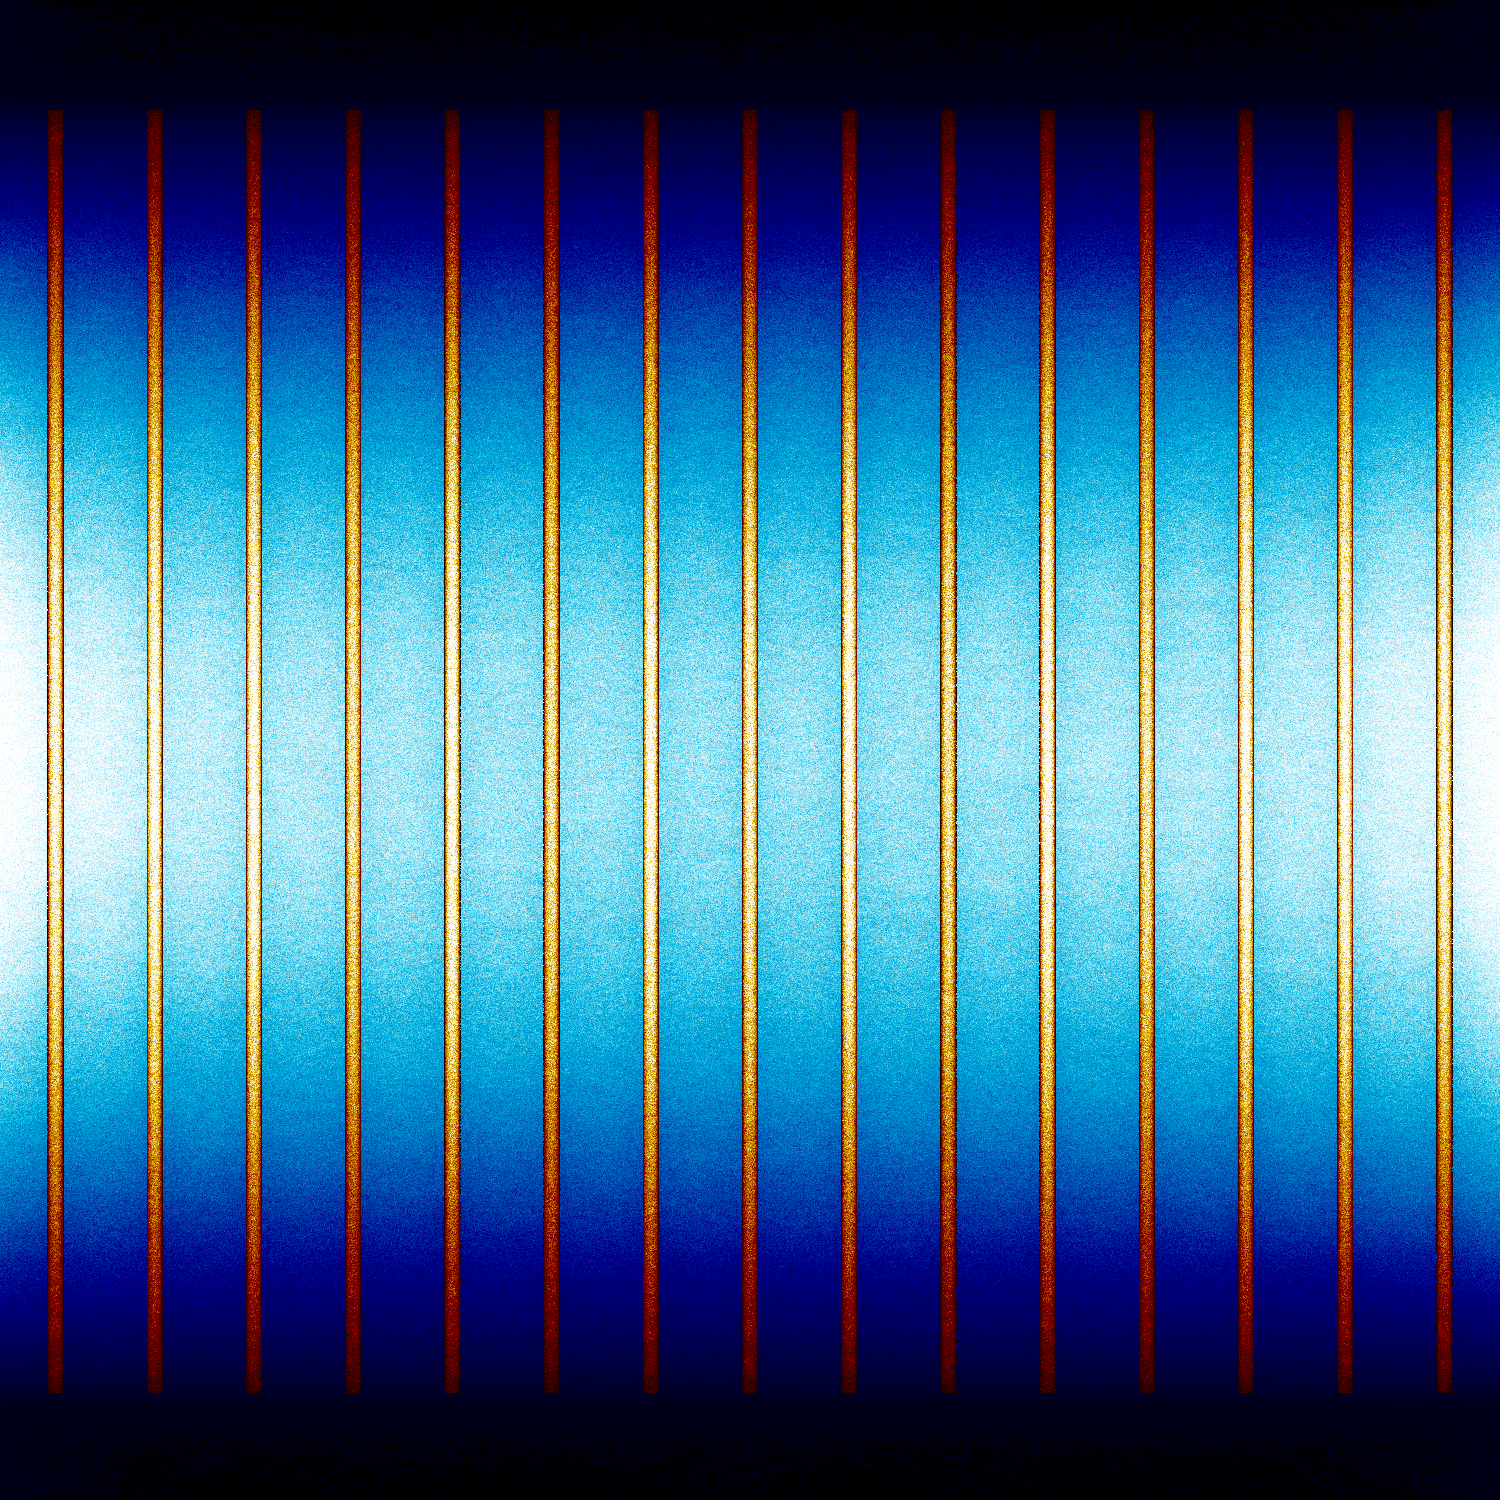
\includegraphics[width=\linewidth]{figs/powerdist-donothing.png}
        \caption{Baseline --- cosine-shaped power profile peaked at the axial midplane, with reduced flux at the rod extremities due to neutron leakage.}
        \label{fig:powerdist_baseline}
    \end{subfigure}
    \hfill
    \begin{subfigure}[t]{0.48\linewidth}
        \centering
        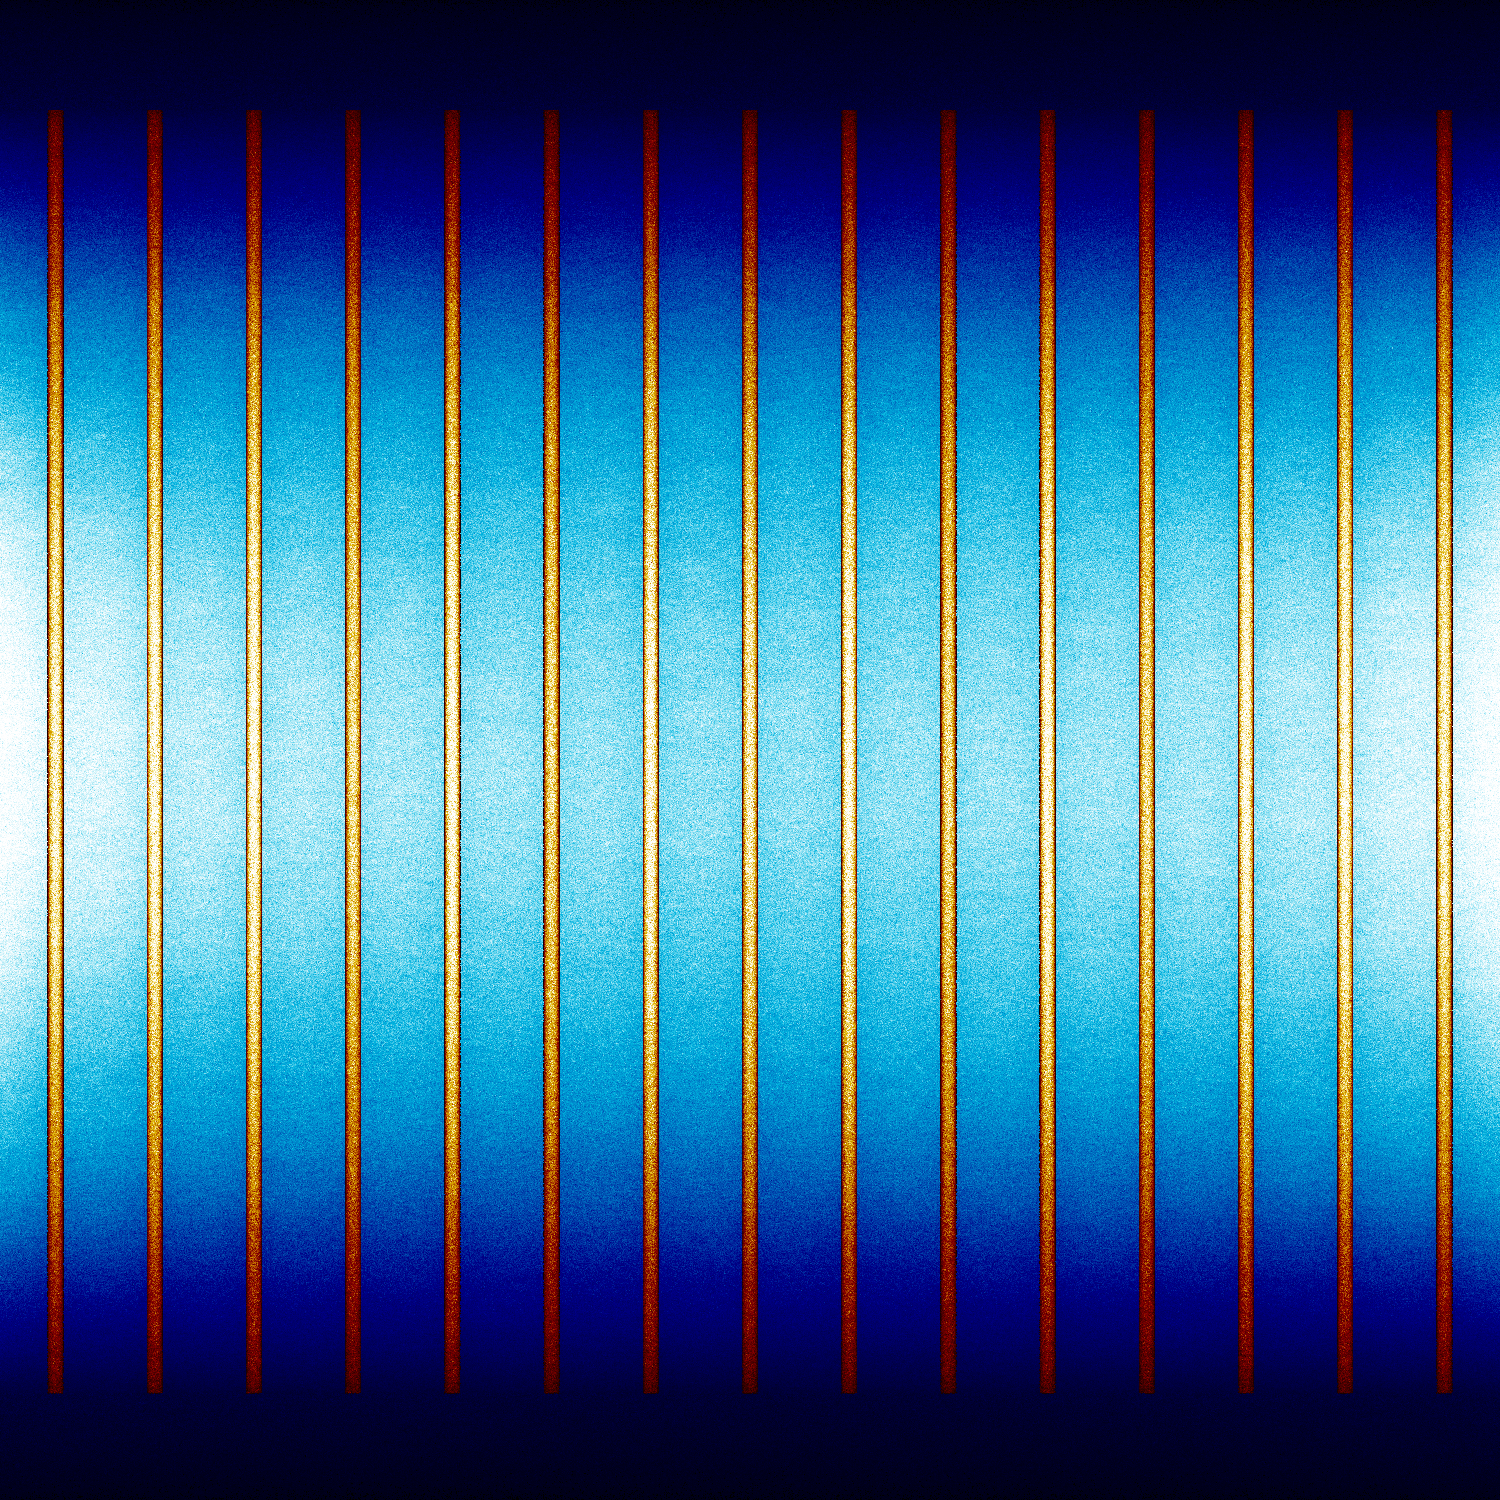
\includegraphics[width=\linewidth]{figs/powerdist-becaps.png}
        \caption{Beryllium End Reflectors --- minimal redistribution relative to the baseline; the cosine shape is largely preserved, indicating limited effectiveness of passive end-reflection.}
        \label{fig:powerdist_becaps}
    \end{subfigure}

    \medskip

    \begin{subfigure}[t]{0.48\linewidth}
        \centering
        
\includegraphics[width=\linewidth]{figs/powerdist-freshrods.png}
        \caption{Fresh Fuel Rods --- elevated and asymmetric power distribution driven by the graded enrichment of the interleaved fresh rods; power remains center-heavy with a shifted axial profile.}
        \label{fig:powerdist_freshrods}
    \end{subfigure}
    \hfill
    \begin{subfigure}[t]{0.48\linewidth}
        \centering
        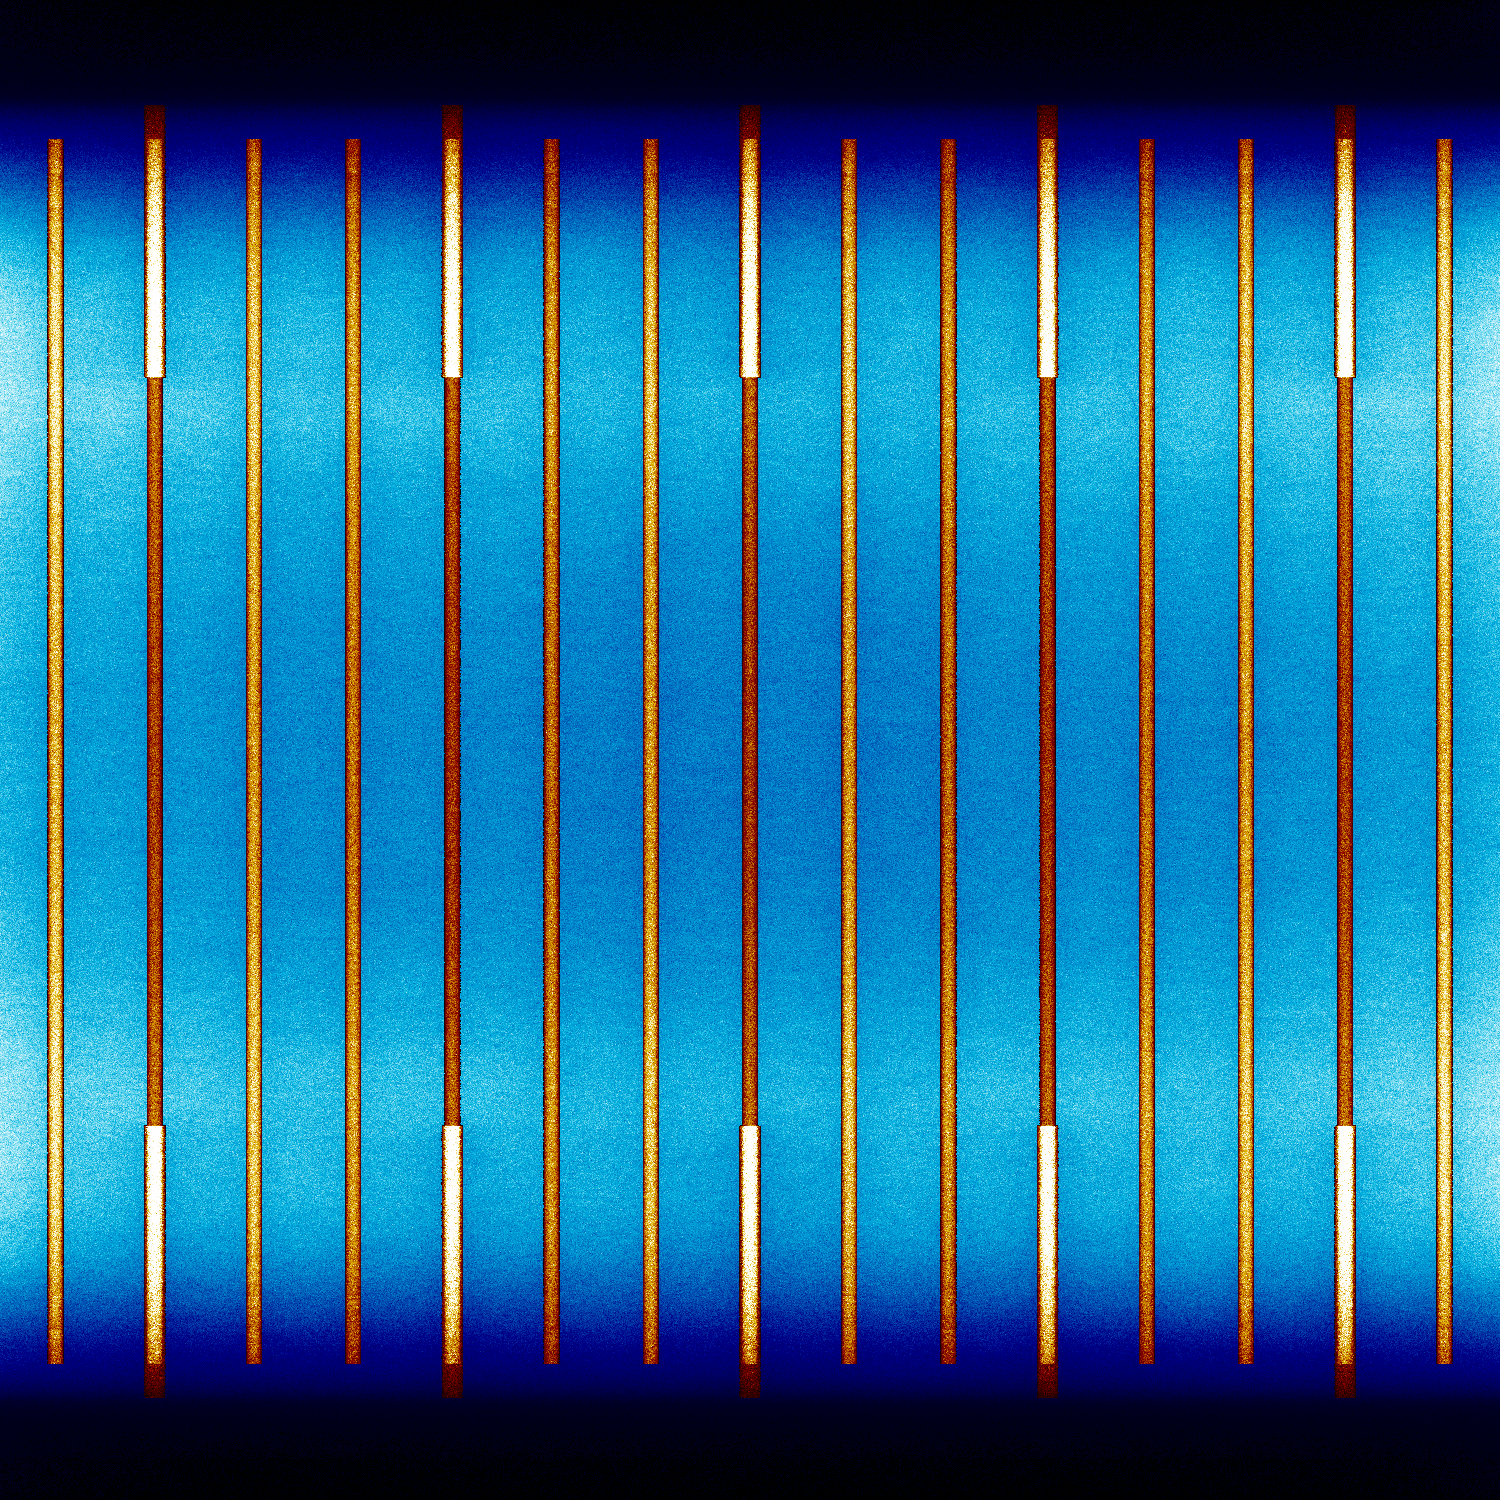
\includegraphics[width=\linewidth]{figs/powerdist-powerinverter.png}
        \caption{Power Inverter Device --- distinctly inverted power profile. The UO$_2$ end regions of the Power Inverter rods produce localized high-flux zones at the axial extremities, while the CeO$_2$ central region yields a dark (low-power) band in the core midplane.}
        \label{fig:powerdist_powerinverter}
    \end{subfigure}

    \caption{Axial power distribution maps for each design variant, rendered as Serpent flux tallies over the assembly cross-section. Brighter color indicates higher local neutron flux and power density. Each image is normalized independently.}
    \label{fig:power_dist_all}
\end{figure}




\clearpage
\section{TMI-1 NJ05YU Spent Fuel Reference Data (D. Frank)}
\label{sec:app_C}
\begin{table}[H]
\centering
\caption{Nuclide c Fractions}
\begin{tabular}{lr|lr}
\hline
\textbf{Nuclide} & \textbf{Mass Fraction} & \textbf{Nuclide} & \textbf{Mass Fraction} \\
\hline
Ag-109 & 6.027$\times10^{-5}$ & Pu-238 & 4.231$\times10^{-4}$ \\
Am-241 & 4.682$\times10^{-4}$ & Pu-239 & 4.605$\times10^{-3}$ \\
Am-243 & 1.805$\times10^{-4}$ & Pu-240 & 2.349$\times10^{-3}$ \\
Am-242m & 1.550$\times10^{-6}$ & Pu-241 & 1.226$\times10^{-3}$ \\
Cs-137 & 1.626$\times10^{-3}$ & Pu-242 & 8.597$\times10^{-4}$ \\
Eu-151 & 6.486$\times10^{-7}$ & Rh-103 & 5.669$\times10^{-4}$ \\
Eu-153 & 1.591$\times10^{-4}$ & Ru-101 & 1.081$\times10^{-3}$ \\
Eu-155 & 9.193$\times10^{-6}$ & Sm-147 & 2.111$\times10^{-4}$ \\
Gd-155 & 8.682$\times10^{-6}$ & Sm-149 & 3.098$\times10^{-6}$ \\
Mo-95 & 1.013$\times10^{-3}$ & Sm-150 & 3.864$\times10^{-4}$ \\
Nd-143 & 9.537$\times10^{-4}$ & Sm-151 & 1.226$\times10^{-5}$ \\
Nd-145 & 8.682$\times10^{-4}$ & Sm-152 & 1.200$\times10^{-4}$ \\
Nd-148 & 5.278$\times10^{-4}$ & Tc-99 & 1.252$\times10^{-3}$ \\
Np-237 & 6.333$\times10^{-4}$ & U-234 & 1.668$\times10^{-4}$ \\
O-16 & 1.185$\times10^{-1}$ & U-235 & 5.746$\times10^{-3}$ \\
 & & U-236 & 4.784$\times10^{-3}$ \\
 & & U-238 & 8.512$\times10^{-1}$ \\
\hline
\end{tabular}
\label{tab:nuclide_mass_fractions}
\end{table}


\begin{table}[H]
\centering
\caption{TMI-1 Reactor Rod H6 (Fuel-1) Characteristics}
\begin{tabular}{ll}
\hline
\textbf{Parameter} & \textbf{Value} \\
\hline
Rod identifier & H6 \\
Rod type & Fuel-1 \\
Rod diameter & 10.922 mm \\
Rod active fuel length & 360.17 cm \\
Fuel Density & 10.196 cm \\
Fuel pellet inner diameter & -- \\
Fuel pellet outer diameter & 0.936 cm \\
Clad inner diameter & 0.958 cm \\
Clad outer diameter & 1.092 cm \\
Cladding material & Zircaloy-4 \\
Cladding density & -- \\
Cladding temperature & 640 K \\
Total rod length & 390.804 cm \\
Active length & 360.172 cm \\
Rod in irradiation cycles & Cycle 9 (Up: 666 d, Down: 36 d) \\
 & Cycle 10 (Up: 692 d, Down: 34 d) \\
\hline
\end{tabular}
\label{tab:tmi1_rod_characteristics}
\end{table}

\begin{table}[H]
\centering
\caption{TMI-1 Reactor H6 Fuel Rod Burnup Distribution}
\small
\begin{tabular}{lccc}
\hline
\textbf{Sample ID} & \textbf{U-235 wt\%} & \textbf{Burnup (GWd/tHM)} & \textbf{Pos. from Plug (mm)} \\
\hline
A1B & 4.01 & 44.8 & 282.85 \\
A2 & 4.01 & 50.6 & 746.76 \\
B3J & 4.01 & 53.0 & 770.13 \\
B2 & 4.01 & 50.1 & 1150.62 \\
B1B & 4.01 & 54.5 & 1559.56 \\
C3 & 4.01 & 51.3 & 1562.10 \\
C2B & 4.01 & 52.6 & 1946.15 \\
C2D1 & 4.01 & 53.5 & 1972.00 \\
C2D2 & 4.01 & 52.7 & 2332.00 \\
C1 & 4.01 & 50.2 & 2354.58 \\
D1A2 & 4.01 & 55.7 & 2618.99 \\
D1A4 & 4.01 & 50.5 & 2923.79 \\
D2 & 4.01 & 44.8 & 3220.72 \\
\hline
\end{tabular}
\label{tab:tmi1_burnup_distribution}
\end{table}


\end{document}